\documentclass[12pt, a4paper, twoside]{book}

\usepackage{helvet}
\usepackage{hyperref}
\usepackage{graphicx}
\usepackage{listings}
\usepackage{textcomp}
\usepackage[
	a4paper,
	outer=2cm,
	inner=4cm,
	top=2cm,
	bottom=2cm
]{geometry}
\usepackage{float}
\usepackage{tabularx}
\usepackage[disable]{todonotes}
\usepackage{color, soul}
\usepackage{amsmath}
\usepackage{algorithmicx}
\usepackage[noend]{algpseudocode}
\usepackage{algorithm}
\usepackage{framed}
\usepackage{subcaption}
\usepackage{titlepic}
\usepackage{fancyhdr}
\usepackage[simplified]{styles/pgf-umlcd}
\usepackage{shorttoc}
\usepackage{url}
\usepackage{paralist}
\usepackage{dirtytalk}
\usepackage{verbatim}

\definecolor{grey}{rgb}{0.9, 0.9, 0.9}
\definecolor{dkgreen}{rgb}{0,0.6,0}
\definecolor{dkred}{rgb}{0.6,0,0.0}

\lstdefinestyle{DOS}
{
    backgroundcolor=\color{black},
    basicstyle=\scriptsize\color{white}\ttfamily,
    stringstyle=\color{white},
    keywords={}
}

\lstdefinestyle{makefile}
{
    numberblanklines=false,
    language=make,
    tabsize=4,
    keywordstyle=\color{red},
    identifierstyle= %plain identifiers for make
}

\lstset{
  language=Python,                % the language of the code
  escapeinside={\%*}{*)},
  basicstyle=\footnotesize\ttfamily,
  numbers=left,                   % where to put the line-numbers
  stepnumber=1,                   % the step between two line-numbers. If it's 1, each line
  numbersep=5pt,                  % how far the line-numbers are from the code
  backgroundcolor=\color{white},      % choose the background color. You must add \usepackage{color}
  showspaces=false,               % show spaces adding particular underscores
  showstringspaces=false,         % underline spaces within strings
  showtabs=false,                 % show tabs within strings adding particular underscores
  frame=single,                   % adds a frame around the code
  rulecolor=\color{black},        % if not set, the frame-color may be changed on line-breaks within not-black text (e.g. comments (green here))
  tabsize=2,                      % sets default tabsize to 2 spaces
  captionpos=b,                   % sets the caption-position to bottom
  breaklines=true,                % sets automatic line breaking
  breakatwhitespace=false,        % sets if automatic breaks should only happen at whitespace
  keywordstyle=\color{blue},          % keyword style
  commentstyle=\color{dkgreen},       % comment style
  stringstyle=\color{dkred},         % string literal style
  columns=fixed,
  extendedchars=true,
  frame=single,
}

%\renewcommand{\chaptername}{Topic}

% New definitions
\algnewcommand\algorithmicswitch{\textbf{switch}}
\algnewcommand\algorithmiccase{\textbf{case}}
\algnewcommand\algorithmicassert{\texttt{assert}}
\algnewcommand\Assert[1]{\State \algorithmicassert(#1)}%
% New "environments"
\algdef{SE}[SWITCH]{Switch}{EndSwitch}[1]{\algorithmicswitch\ #1\ \algorithmicdo}{\algorithmicend\ \algorithmicswitch}%
\algdef{SE}[CASE]{Case}{EndCase}[1]{\algorithmiccase\ #1}{\algorithmicend\ \algorithmiccase}%
\algtext*{EndSwitch}%
\algtext*{EndCase}%

\pagestyle{fancy}
\fancyhf{}
\fancyhead[RO, LE]{\small \rightmark}
\fancyfoot[RO, LE]{\small \thepage}

\newcommand{\blank}[1]{\hspace*{#1}}

\begin{document}

\frontmatter

\begin{titlepage}
\vspace*{5cm}
\begin{center}

\includegraphics[width=.5\textwidth]{images/EdNapUniLogoCMYK}~\\[1cm]

\textsc{\Large Edinburgh Napier University}\\[1.5cm]

\textsc{\LARGE \bfseries SET08114 Mobile Application Development}\\[0.5cm]

\hrulefill \\[0.4cm]
{\huge \bfseries Notes \& Workbook \\[0.4cm] }
\hrulefill \\[1.5cm]

\begin{minipage}{0.4\textwidth}
\begin{flushleft} \large
\textbf{Dr Simon Wells} \\
\end{flushleft}
\end{minipage}

\vfill

\end{center}
\end{titlepage}

\shorttoc{Overview}{0}

\setcounter{tocdepth}{2}
\cleardoublepage
\tableofcontents
\listoffigures
%\listofalgorithms
\addtocontents{toc}{~\hfill\textbf{Page}\par}

\mainmatter
%\part{Admin}


\part{Labs \& Practical Work}

\chapter{Getting Started}
\label{lab1}
\paragraph{} With the practical portion of this module we aim to learn about the functionality offered by the Android platform. We will treat each functionality as a building block which can be combined with other blocks, and glued together using the Java language to build our own apps. Throughout the practical labs we will explore these blocks and begin to combine them in simple ways. In your coursework assignment you will then have the opportunity to use these skills to design and implement an app of your own.

\begin{framed}
\paragraph{IMPORTANT} The libraries that make up the android platform are being continuously developed. Each new release is assocated with an API level. Higher API levels usually introduce changes that either break or deprecate working code from earlier level. The workbook currently targets API level 21 (codenamed Lollipop). \emph{If you want to develop for a later API level, such as Marshmallow or Nougat, in order to take advantage of more advanced features, particularly for your coursework assignment, then there may be instances of broken or deprecated code between the examples in the workbook and the android platform libraries.} However, for the core learning on this module we will assume that all of our development targets no lower than API level 21.
\end{framed}

\section{Aims}
\paragraph{} At the end of the practical portion of this topic you will be able to:

\begin{itemize}
\item Install the android development tools (OPTIONAL: Only if you have your own machine)
\item Create a default `Hello Android' application
\item Create an AVD for running your application
\end{itemize}

\paragraph{} We will use Android Studio to develop mobile applications on this module. Android Studio is an Integrated Development Environment (IDE) for managing the writing, testing, and running of Android applications. IDEs like Android Studio have many advantages when starting out with Android development. A lot of early activities when learning about Android is related to finding out what the platform offers. With an IDE there is usually a window or some code-completion that makes suggestions so that, over time, you become more familiar with the options available to you. There are particular advantages to using the command-line which are important, for example, when large teams of developers are working within a professional environment to collaboratively build applications. However, in this module we will concentrate on using an IDE.

\begin{framed}
\paragraph{IMPORTANT} \emph{This introductory practical is the only one which will describe in detail the process of creating a new project. All subsequent labs will assume that you can achieve this for yourselves. If in doubt refer back to this practical. It will be your responsibilty to explore and become familiar with your development environment so that you can at least perform basic tasks.}
\end{framed}

\begin{framed}
\paragraph{IMPORTANT} The code examples in the workbook are all included as source code in the module Git repository which can be found at: \url{https://github.com/siwells/teaching_set08114}. The workbook tries to focus on important aspects and fragments of a given topic but should not be used in isolation, rather, use the workbook to focus on fragments of the topic and the examples in the repository to see the fragment in the context of a full working app.
\end{framed}

\section{Say ``Hello Android''}
\label{hello}
\paragraph{} With an IDE there is a lot of initial hand-holding available to help get you started. In fact, to run a ``Hello World'' or more appropriately ``Hello Android'' app requires no code to be written at all. The entire app is generated ready to be compiled, installed, and run on an appropriate Android device such as connected hardware, emulator, or a virtual device. This is very useful because, depending upon the options that you select when you create a new app project, the basic scaffold for your app is automatically generated for you and is \emph{ready to run}, i.e. if you don't break it then Android Studio gives you a fresh, ready to run app (that does nothing very much). 

\paragraph{} This worksheet aims to give a pictorial introduction to the process of creating a first ``Hello Android'' application using Android Studio as your IDE. Studio actually does nearly all of the work for you and most of the time, at this stage in the module, all you need to do is {\bf{accept the defaults}}. So let's start by launching Android Studio.

\paragraph{} Use the `Quick Start' options in the right-hand pane and click `Start a new Android Studio project' as shown in Figure \ref{fig:android.studio_welcome}.

\begin{figure}[H]
\centering
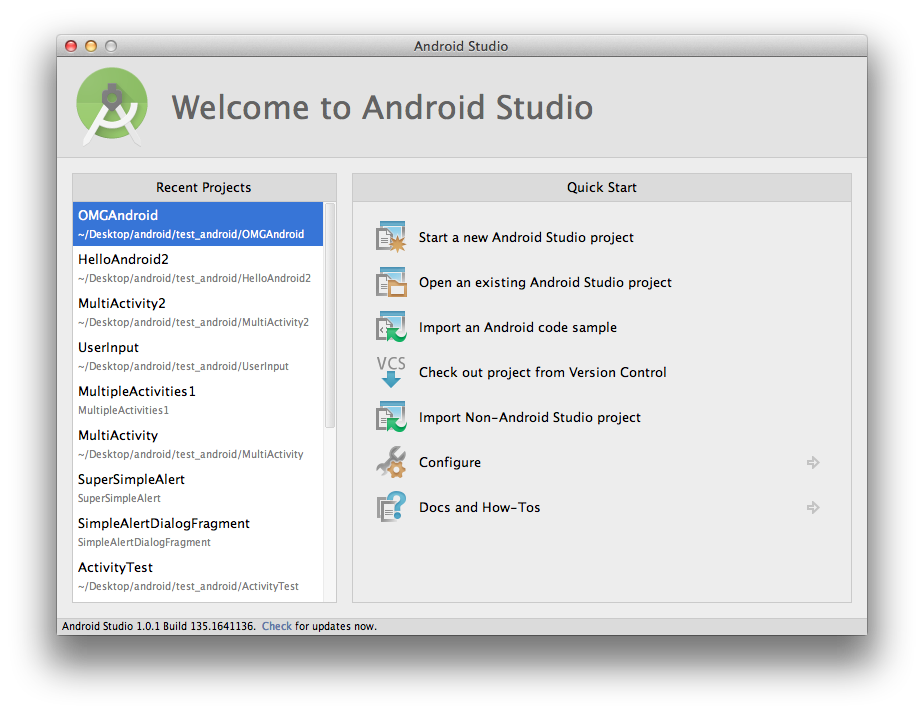
\includegraphics[width=\textwidth]{images/android-studio_01_welcome}
\caption{Android Studio welcome pane}
\label{fig:android.studio_welcome}
\end{figure}

\paragraph{} You should see the window shown in Figure \ref{fig:android.studio_config}. Enter a name for your new Application. This will also be used for your project name. For our first app let's call it `HelloNapier'. For `Company Domain' I suggest you enter `napier.ac.uk'. Now click Next to continue.

\begin{figure}[H]
\centering
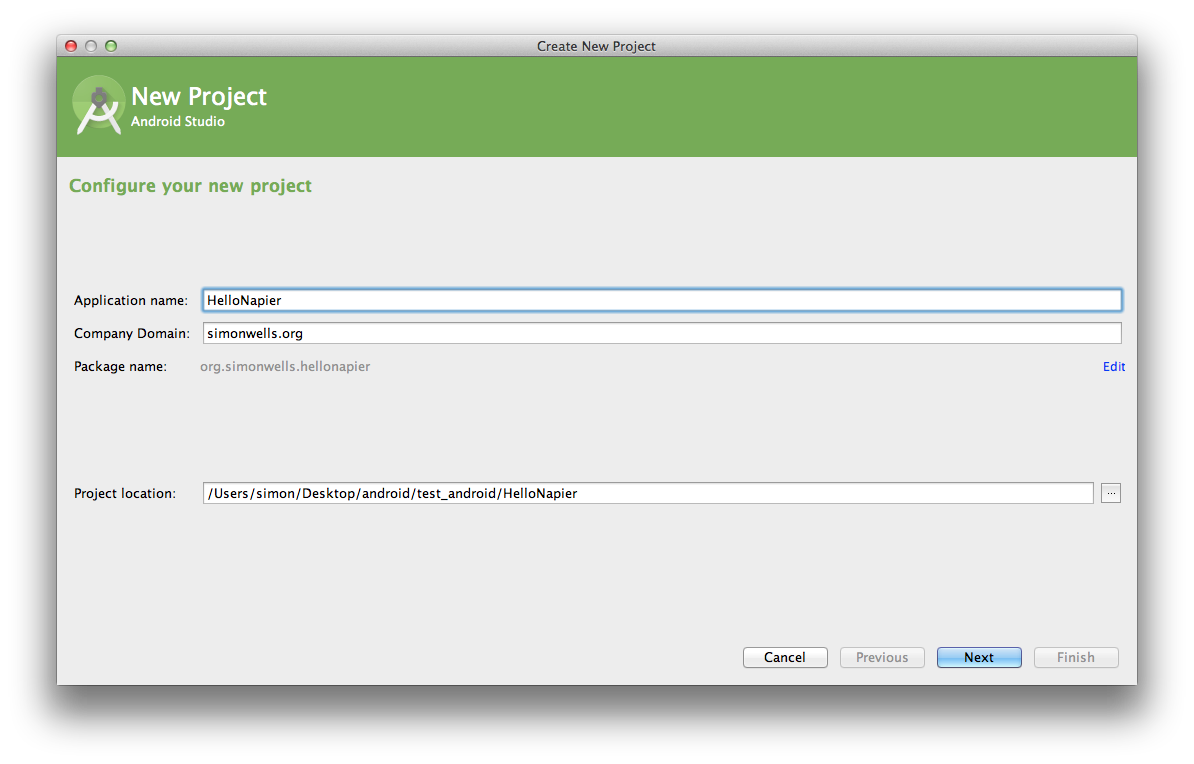
\includegraphics[width=\textwidth]{images/android-studio_02_configure}
\caption{Android Studio new app configuration pane}
\label{fig:android.studio_config}
\end{figure}

\paragraph{} On this screen, accept the defaults for now. NB. These should be as shown in Figure \ref{fig:android.studio_form}. Now click Next.

\begin{figure}[H]
\centering
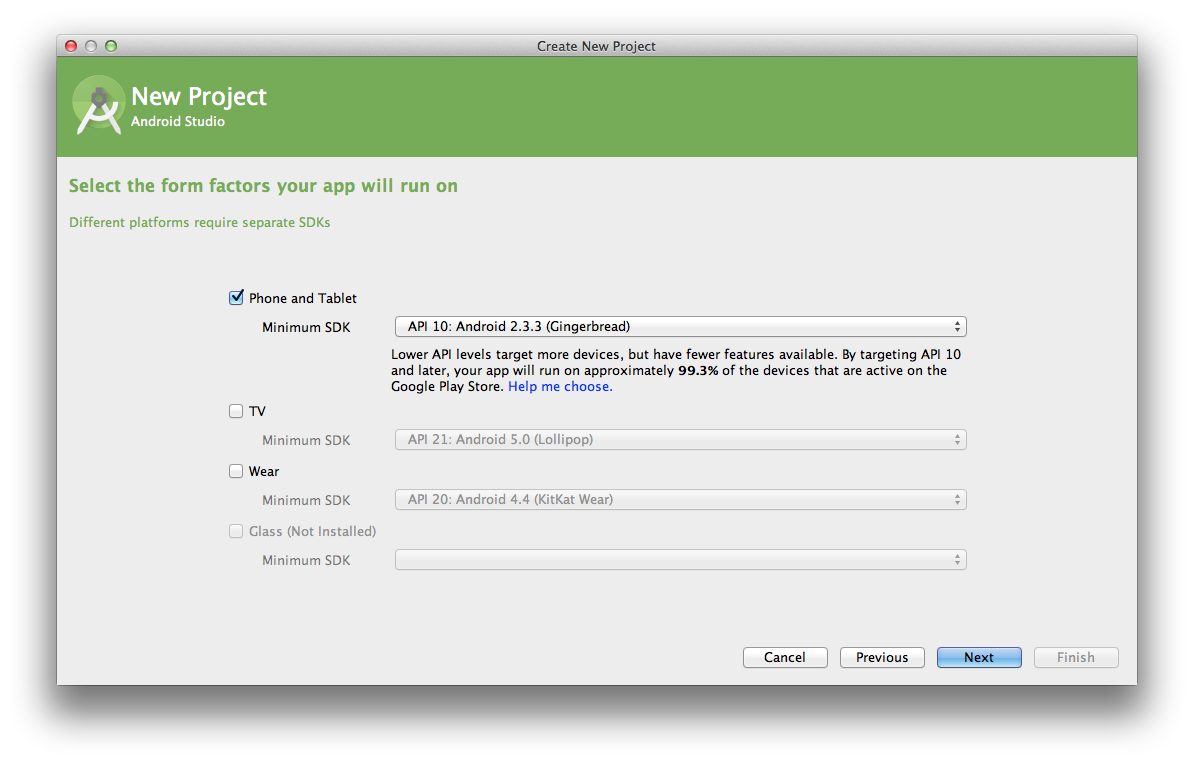
\includegraphics[width=\textwidth]{images/android-studio_03_form-factors}
\caption{Android Studio form factor selection pane}
\label{fig:android.studio_form}
\end{figure}

\paragraph{} Again, accept the default, `Blank Activity', which should be highlighted, then click Next.

\begin{figure}[H]
\centering
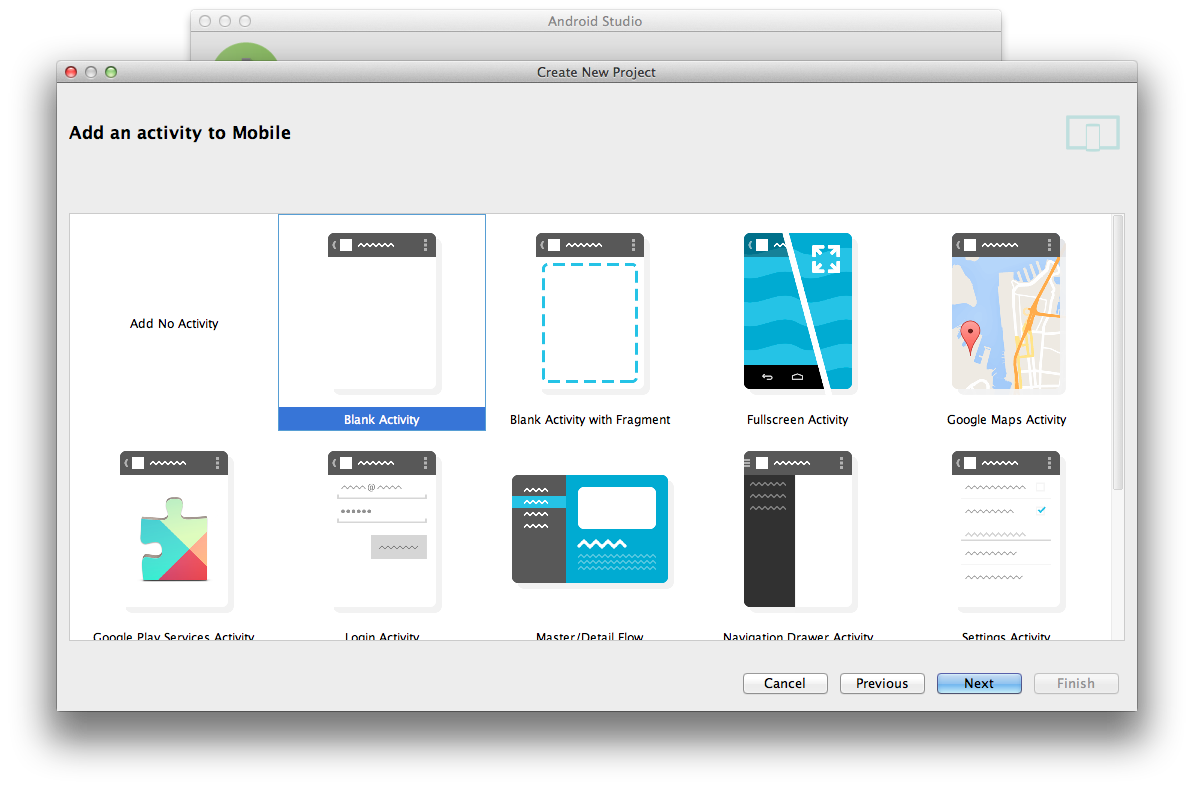
\includegraphics[width=\textwidth]{images/android-studio_06_activity}
\caption{Android Studio activity setting pane}
\label{fig:android.studio_activity}
\end{figure}

\paragraph{} Accept the defaults on this screen for now and click Next again.

\begin{figure}[H]
\centering
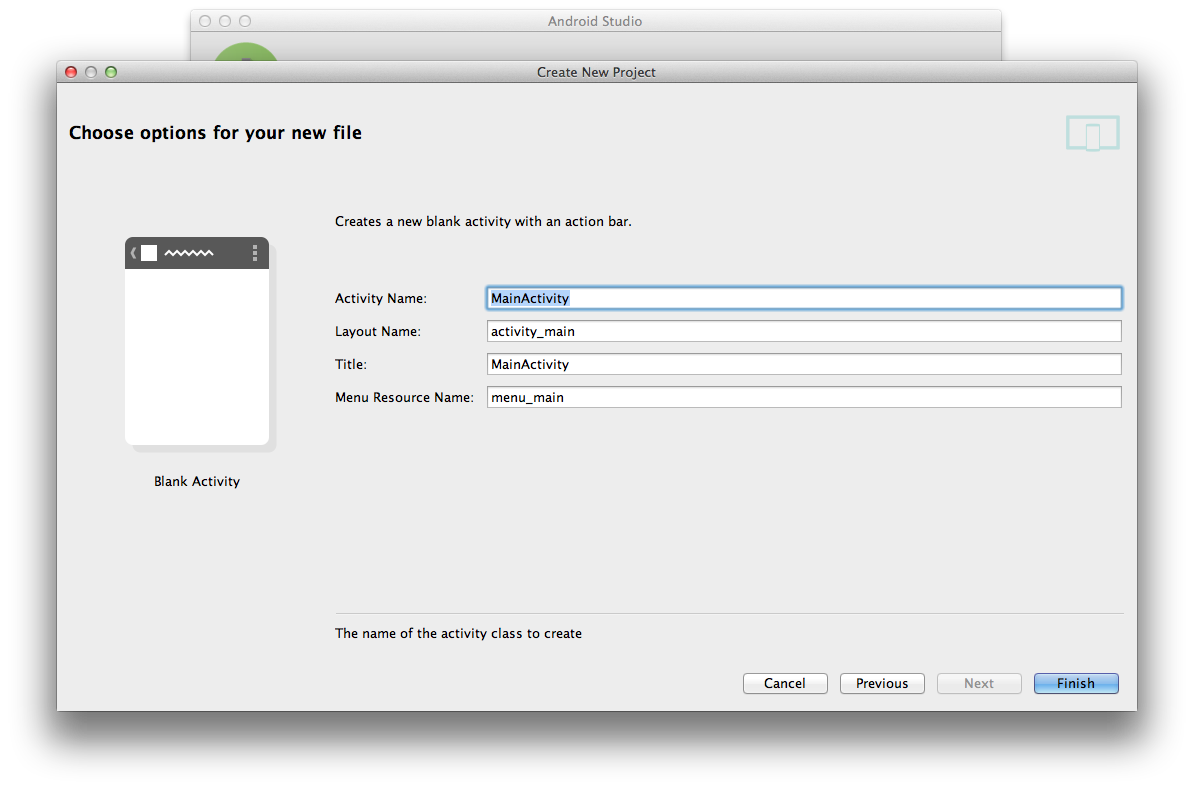
\includegraphics[width=\textwidth]{images/android-studio_07_options}
\caption{Android Studio options pane}
\label{fig:android.studio_options}
\end{figure}

\paragraph{} After a brief pause, whilst your machine loads all of the relevant libraries and creates your project file, you should be presented with the Android Studio workspace as shown in Figure \ref{fig:android.studio_studioui}.

\paragraph{NB.} It can take a while for your new project to load completely which depends upon the speed of your machine. If there are any errors or warnings on screen, especially in the preview window which renders waht your Android app interface will look like, then your project hasn't loaded completely yet.

\begin{figure}[H]
\centering
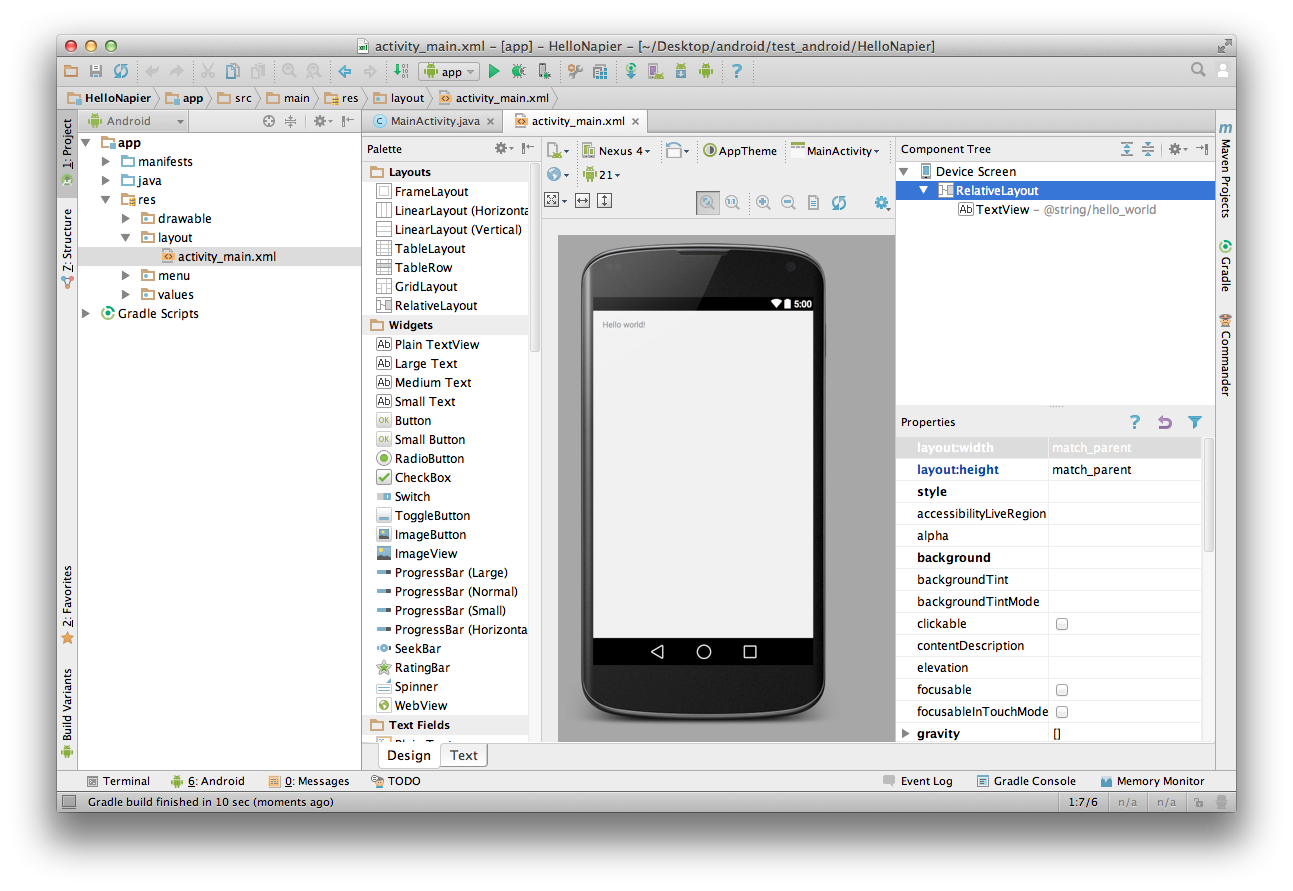
\includegraphics[width=\textwidth]{images/android-studio_08_studio-ui}
\caption{Android studio UI with default Android app}
\label{fig:android.studio_studioui}
\end{figure}

\paragraph{} Congratulations. You just created a New Android Studio projectThis process can be summarised as follows:

\begin{enumerate}
\item Click `Start a new Android Studio project'
\item Type in an application name \& Company Domain (napier.ac.uk) then click `Next'
\item Select an API level
\item Ensure `Blank Activity' is selected then click `Next'
\item Click Finish
\end{enumerate}

\paragraph{} Now you have created your first Android project. Whenever we say `Create a new project' we mean go though steps 1 to 5 ({\bf{you will have to either give each new project a different name or else save them to different locations}}).

\paragraph{} It is worth going through this process several times to become familiar with it. Once you have done it half a dozen times or so you should become comfortable with the idea of creating a new Android project and it shouldn't take more than a few seconds.

\paragraph{} It is also worth exploring some of the options that the project creation wizard offers. In particular it is worth exploring the API levels page to see what the differences are between the different API levels supported by Android. When you are on the form factors page shown in Figure \ref{fig:android.studio_form} click the link to ``Help me choose''. This will cause the API Level window to be displayed which is illustrated in Figure \ref{fig:android.studio_apilevel}.

\begin{figure}[H]
\centering
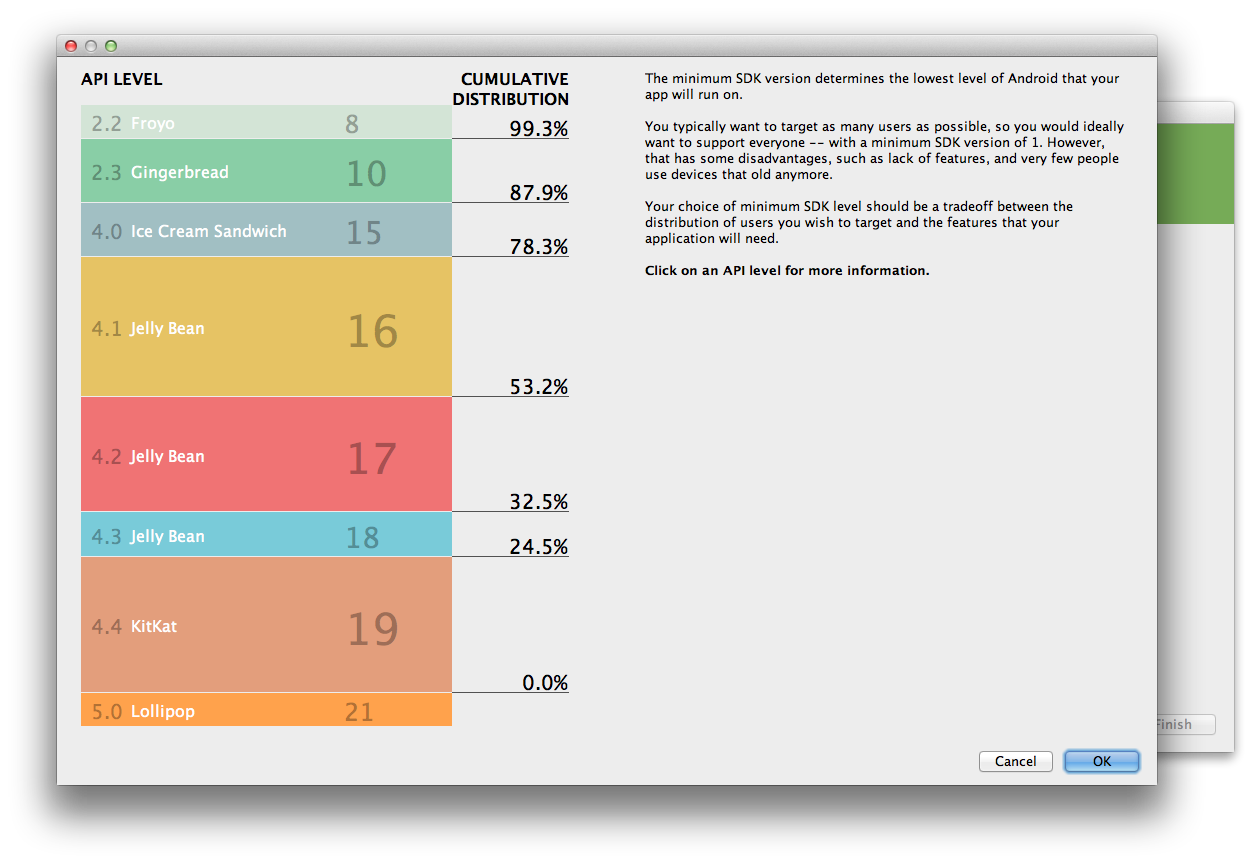
\includegraphics[width=\textwidth]{images/android-studio_04_api-level}
\caption{Android Studio API level selection screen}
\label{fig:android.studio_apilevel}
\end{figure}


\paragraph{} This page gives you an idea of the proportion of the market for Android devices that you can target with each API level. If you click on a particular level, e.g. `2.3 Gingerbread' then you will see extra information about the features offered by that verson of Android. Remember, higher API levels support newer or more refined features whereas lower levels are supported by a wider proportion of the population of Android devices. Choosing an API level is therefore partly a technical decision, because it affects what you can do, partly a business decision, because it affects the size of your potential customer base, and partly an aesthetic decision, because how things are displayed is also affected by API level. So choose wisely ;) 

\begin{figure}[H]
\centering
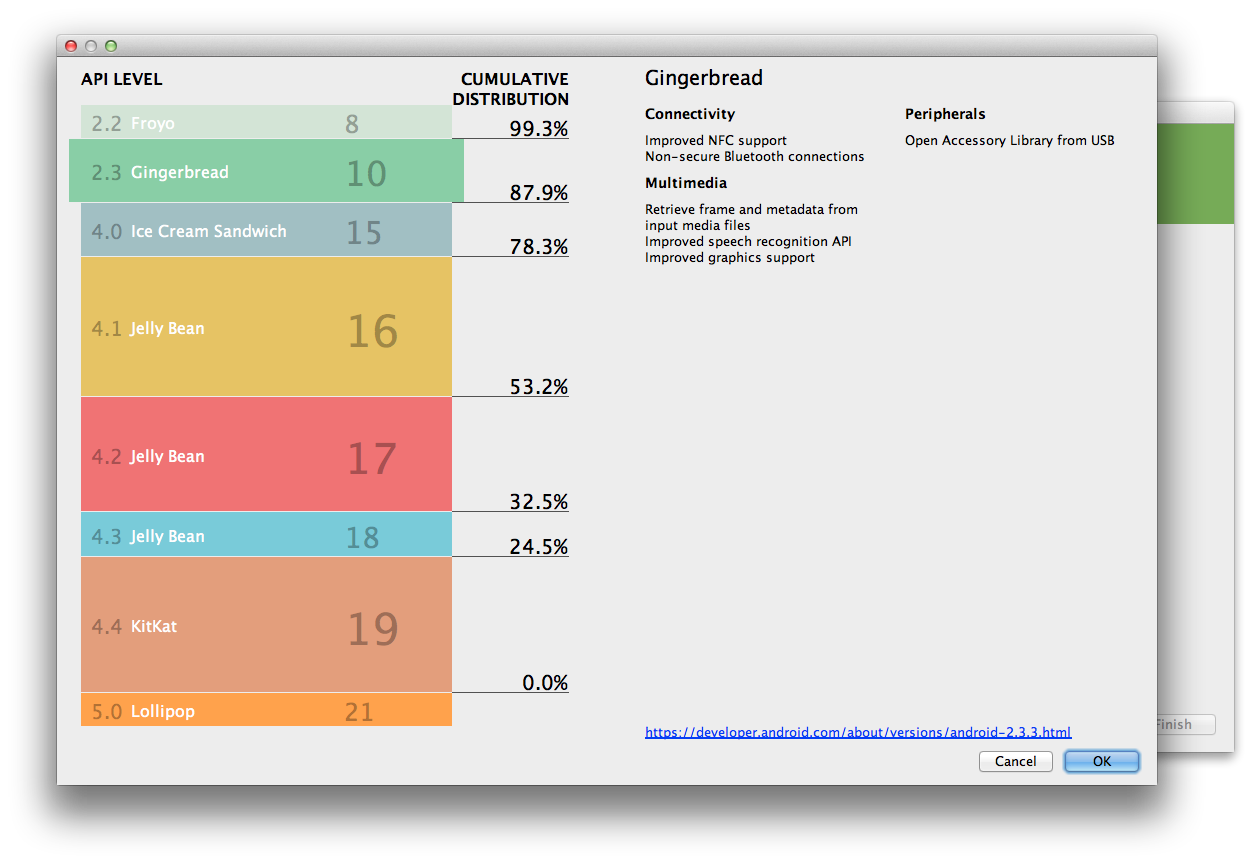
\includegraphics[width=\textwidth]{images/android-studio_05_api-level-details}
\caption{Android Studio API level details screen}
\label{fig:android.studio_apidetails}
\end{figure}

\paragraph{} It can take quite a while, even minutes, for Android Studio to completely load your new project and all of the supporting libraries. If the preview of the Android UI isn't fully displayed or has a message on it then Android Studio is still loading and compiling things so it is best to let it finish. Similarly if there are errors or warnings in the ``Problems'' tab then it is likely that these are due to your IDE still loading and building resources. Sometime the IDE can also get ahead of itself and tries to use one component before another is properly loaded. Usually when this occurs there will be a message with a link to let you reload or retry the component. When we build a new Android Studio project, especially for the first time, there will be a lot of code to generate and libraries to link, and this can take a while. Also, because everyone in the class is trying to do this at the same time, and Android Studio runs across the university network from the ``U:\'' drive there can be some significant lag. At this point you should just wait for things to resolve themselves. You imght also notice, in the status bar of Android Studio, that there is a message regarding scanning or indexing files, this happens when we first use Android Studio, it can take a while to complete, and it can cause significant performance issues initially.

\paragraph{} Now you need to build and run your app. This is important because we want to actually see our app running and doing something don't we?

\section{Running our app using Android Virtual Devices (AVDs)}
\label{avd}
\paragraph{} Because Android apps are not Windows (or Linux, or MacOS) apps they will not usually run natively on our operation systems (unless you are using Android as your OS but let's ignore that case for now). That means that you cannot just double click on your app and have it run in a window. Android apps rely on the Android OS to provide not just the platform libraries that contain all the code you didn't write but also all of the app management functionality. Android apps are a collection of activities (we will talk about these in class next week) and the OS manages when to display a given activity and when to allow another activity to take precedence. As a result we need a way to run our Android app. There are three alternatives, you can use a hardware device plugged into your computer via USB, or you can emulate the hardware of an Android device. Android devices usually run on an ARM architecure, which is different to most desktop machines, and thus that architecture needs to be emulatedin software, this can be very slow. A third option is to use a virtual device that runs a version of the Android OS that is built for the x86 architecture. This allows us to use real hardware, e.g. CPU cores and RAM, to run the Android OS in the virtual device. We can then load our Android app in this virtual version of Android and have it run with acceptable performance. This approach is known as using an `Android Virtual Device' (AVD) and we interact with AVDs through the AVD manager. We can access this through the Tools $\to$ Android $\to$ AVD Manager menu option. The AVD manager lets you set up multiple AVDs, e.g. targetting different versions of Android or simulating different hardware capabilities. For the moment we should merely use the default AVD and accept the defaults that the AVD manager suggests. Bare in mind that an AVD is quite large, around 650MB each, so you might not want to create too many of them. Currently AVDs are stored in the C: drive of the JKCC machines so each time you use a different machine you will probably have to create a new AVD. This is a known ``feature'' of the JKCC which is being worked on. 

\paragraph{} Once you have created a new Android device then it it needs to be started. As this process is essentially starting up a whole operating systems this can take a few moment. Eventually however you should see a new window that looks a bit like an Android device

\paragraph{} Once you have an AVD created you can select the Run $\to$ Run `app' menu optionand your Android app will be built and tranferred to your AVD. You might have to select the AVD that you want to run the app in from a list of running devices. NB. If you have attached a harware device to your computer using USB then this device should also be listed however there are some caveats; you will need to have the correct drivers installed for your device and this will probably not work in the JKCC with your own device but should be OK on your own laptop.

\paragraph{} That's it for this week. You should get yourself \emph{very} comfortable with these processes and go through them multiple times as every app that you will build during the mdule, and you will build tens if not hundreds of apps, will require you to set up a new project. You should only need a single AVD using the default settings for the majority of the lab exercises. If other settings are required for a particular exercise then this will be flagged as necessary. That said, experiment with Android studio, explore some of the features that it offers, and get as familar as you can with it so that you are ready to do more in subsequent labs.



\chapter{Baby Steps with Android}

\section{Aims}
\paragraph{} At the end of the practical portion of this topic you will be able to:

\begin{itemize}
\item Understand the basic relationship between Android project files
\item Display text using an Android View
\item Display buttons and respond when they are used
\item Display notifications (Toasts) to users
\item Log output from your app and view it using logcat
\end{itemize}

\section{Preliminaries}
\paragraph{} Create a new Android project using the process we followed for HelloAndroid. You should give your project a different name, for example, `HelloString' (because to begin with we shall be manipulating the strings that say Hello ;). It is a good idea to come up with a naming scheme for your Android projects or perhaps to organise them in folders based upon module topic or semester week number so that later in the course you can refer back to earlier code you have developed.

\paragraph{} In Android Studio open the Activity Java file. This should be called `MainActivity.java' and will be located in the 
\begin{framed}
src/uk/ac/napier/napier-id/HelloString/ 
\end{framed}
\paragraph{} folder of your project. 

\paragraph{} There isn’t a lot to see here. Most of what you see is commonly called `boilerplate' and is basically setting up the things that the Android libraries need to provide the framework for an empty project. What you will notice is that the things you see on screen when you run this app are not anywhere to be found in this Java file. This is because all the text, graphics, and layout information is created and stored in separate XML files. These XML files are then referenced from the Java code or other XML files. This means that Android has a very flexible development system which encourages well structured and reusable designs but the drawback is that it is a little complicated to get started with.

\paragraph{} There are a few things to take particular note of in the MainActivity.java file.

\begin{lstlisting}
    public class MainActivity extends Activity {
\end{lstlisting}

\paragraph{} In this line we are creating a class, called MainActivity, which inherits from the Activity parent class. Rather than creating a main method like we do in a Java program we are allowing the Android libraries to provide the main method instead. This is because we are not writing a Java program, we are writing an Android app, and these are different things. When we write an Android app we will be working within the framework of classes and libraries provided by the Android platform and there are certain requirements for an Android app to become an Android app. Because the core of an Android app is the Activity we must use the existing Android classes that provide Activity functionality. There are a number of Activity and other classes that we can inherit functionality from but for the moment we will concentrate on the core Activity class.

\paragraph{} Because we have inherited from the Activity base-class we must implement a number of methods that allow our apps functionality to `hook in' to the framework provided by the Android platform. Importantly right now we override the onCreate method. This is the method that pretty much starts the life-cycle of our app. It is called when our app is created and does a lot of work for us. In this case, with our basic HelloString app all it does is call the parent class onCreate method to ensure that the hierarchy of Activity classes are properly initialised then

\begin{lstlisting}
setContentView(R.layout.activity_main);
\end{lstlisting}

\paragraph{} Let's unpack this a little. The setContentView part is a call to a method related to displaying something on screen. We then have the argument to this method which contains 
\begin{framed}
R.layout.activity\_main
\end{framed}
\paragraph{} What this means is that we are referencing an Android resource. `R' is short for resource, notice that in package explore there is a folder called `res'. This contains all of the information about things that our can display, amongst other things. For our purposes we can consider `R' to refer to these resources. In reality it is slightly more complicated because when we build our app the contents of the res folder are assembled into a more efficient representation and the `R' file is essentially an index to our efficient representation of our resources. Going back to our line of code, without the res folder there is a sub-folder called layout, inside of which is a file called `activity\_main.xml'. This line of code is essentially saying display the layout described in activity\_main.xml, so perhaps we should take a look at that file. Use package explorer to open it.

\paragraph{} There is a lot to take in in this file. For a start. it doesn't look like a Java language source file. That is because it isn't. It is an eXtensible Markup Language (XML) file\footnote{\url{http://en.wikipedia.org/wiki/XML}}. XML is used to describe and specify Android resources. There are a number of things happening in this file. The top part

\begin{lstlisting}<RelativeLayout xmlns:android="http://schemas.android.com/apk/res/android"
    xmlns:tools="http://schemas.android.com/tools" android:layout_width="match_parent"
    android:layout_height="match_parent" android:paddingLeft="@dimen/activity_horizontal_margin"
    android:paddingRight="@dimen/activity_horizontal_margin"
    android:paddingTop="@dimen/activity_vertical_margin"
    android:paddingBottom="@dimen/activity_vertical_margin" tools:context=".MainActivity">
\end{lstlisting}

\paragraph{} basically describes a layout for the things to display on screen. Essentially telling Android to use the `Relative Layout' to organise the things that it draws and to use the parameters that are supplied e.g. layout\_height, paddingRight, paddingTop, and paddingBottom. We will see more about layouts and how to arrange things nicely on screen in the next practical so for now we will just ignore it. The next section is more interesting right now:

\begin{lstlisting}    <TextView android:text="@string/hello_world" android:layout_width="wrap_content"
        android:layout_height="wrap_content" />
\end{lstlisting}

\paragraph{} This is interesting because it is the bit that tells the Android platform to display our "Hello World" message. Again, like the use of `R' in MainActivity.java to provide flexibility we have another bit of indirection. Instead of just having all of the strings that our app uses in the place that they are used, instead we have them all collected in a single location, another resource file, called strings.xml which can be found here

\begin{framed}
res/values/strings.xml
\end{framed}

\paragraph{} {\bf{Why do you think that it might be useful to collect all of the strings together in one place?}}

\paragraph{} Our layout file contains a reference to a specific string, stored in the strings.xml resource file, which we want to be displayed onscreen in this layout. The reference is the `@string/hello\_world'. The reference uses `@string' to indicate that the string resource is in the strings.xml file then the name of the resource `hello\_world' to specify the particular string to display. Use package explorer to find and open the strings.xml file.

\begin{lstlisting}
<?xml version="1.0" encoding="utf-8"?>
<resources>

    <string name="app_name">HelloAndroid</string>
    <string name="hello_world">Hello world!</string>
    <string name="action_settings">Settings</string>

</resources>
\end{lstlisting}

\paragraph{} The string that displays the message is the one called `hello\_world'. The content of the string comes between the $<$string name="..."$>$$<$/string$>$ tags, in this cases ``Hello world!''. If you havn't done so yet. Run the project and look at the output. Then try altering the content of the string to display another message of your own design. From here you can even change the name of your app by altering the content of the `app\_name' string but we can leave that alone for now.

\paragraph{} While we have the emulator running we will try using it a bit more, the advanced features of the emulator and how we can interface with it will be covered in a later practical but you should make yourself familiar with what the various buttons on the emulator can do:
•	the home button will return you to the home screen, 
•	the menu button differs with each application and 
•	the back button acts like a browser back button. You will find that the emulator contains the majority of a basic Android phones features, exceptions include Bluetooth and camera as they would require specific hardware.
It is possible to run applications already on the emulator, including our application from earlier. Click the launcher grid button (in the centre of the home screen) and scroll through the list of existing apps, you should be able to find your app and run it from here. To add an app to the home page, press and hold the icon and when the emulator changes to the home page you can drag the icon into place and release it to place it there.

\begin{figure}[H]%[htb]
\centering
    \begin{subfigure}[b]{0.45\textwidth}
        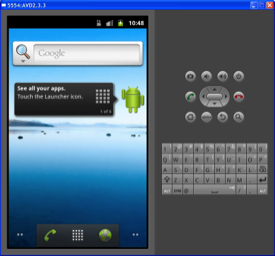
\includegraphics[width=\textwidth]{images/android_home}
        \caption{Android Home}
        \label{fig:android-home}
    \end{subfigure}
    ~ 
    \begin{subfigure}[b]{0.45\textwidth}
        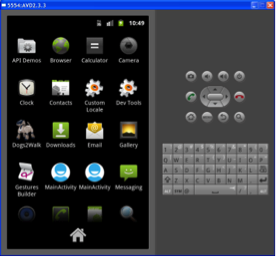
\includegraphics[width=\textwidth]{images/android_apps}
        \caption{Android Apps}
        \label{fig:android-apps}
    \end{subfigure}
\caption{Android home screen \& apps}
\label{fig:android-home-apps}
\end{figure}

\section{The DateTime App}
\paragraph{}Now we have an understanding of how the applications are built and executed on the emulator we will build our first application that does something more than just display the Hello message. Along the way we will explore some of the basic user interface controls available on the Android platform. On Android anything that can be displayed on screen is called a View and this includes all of those elements that we are used to on other platforms that we usually refer to as GUI widgets.

\paragraph{} We're going to create an app which displays the current date and time when you click a button. Create a new app and call it `DateTime'. Open the graphical layout - one way of doing this is simply to double click the activity\_main.xml file in the res/layout folder. You can delete the HelloWorld message, just select it with the mouse and delete it, as we won't be using it.

Your should see an area of the Android Studio UI which provides a `Palette' or `toolbox' of graphical widgets that you can use in your app. Drag a textview view from the palette onto the AndroidApp activity layout. Notice that the graphical layout is a good way to place and arrange Android views on screen to rapidly create a GUI. Select the new Text View – then change the Text property to ``DateTime'' (without the quotes) and the name to ``TextView1''. Click now on the activity\_main.xml tab to see what has happened to the XML code – you should now have a block called <EditText...> like so

\begin{lstlisting}
<TextView
        android:layout_width="wrap_content"
        android:layout_height="wrap_content"
        android:text="DateTime"
        android:id="@+id/textView1"
        android:layout_below="@+id/button1"
        android:layout_centerHorizontal="true" />
\end{lstlisting}

\paragraph{} Now return to graphical layout and select Form Widgets. Drag a button over to your activity layout.  Right click (or double click in Android Studio) to edit the text that goes onto the button - and select Edit Text. You can enter the new text in the field at the bottom (under New String...). Change to ``Click me!''. The default name for your button is button1 – check this by clicking on the button then looking at the properties.

\begin{lstlisting}
<Button
        android:layout_width="wrap_content"
        android:layout_height="wrap_content"
        android:text="Click Me!"
        android:id="@+id/button1"
        android:layout_centerHorizontal="true"
        android:layout_marginTop="79dp"
        android:layout_centerVertical="true" />
\end{lstlisting}

\paragraph{} So we now have a text box and we have a button. Check your app now – select the project from the Package Explorer then click the play button (a green `play' triangle on the menu bar):

\paragraph{} The problem now is that our app doesn't actually do anything. The Click Me! button has no functionality and the TextView will just display DateTime forever. We need to write some code to do something when the button is clicked. We’re going to overwrite the DateTime string with the actual date and time. How are we going to do this? Well, we need to have a handler that will listen for button clicks, we need to write a little bit of code to get the current time and date, and we need a little bit of code to update the TextView with our new time and date.

\paragraph{} Open MainActivity.java. First we need to add some imports so that our app can access the libraries that it needs to do our extra functionality. By default the basic app project only has the minimal set of imports that it needs to display the Hello World message. We have to add other imports to do different things. These are the imports that we need in MainActivity.java in addition to the ones that are already there:

\begin{lstlisting}
import android.view.View;
import android.view.View.OnClickListener;
import android.widget.Button;
import android.widget.TextView;
import java.util.Date;
\end{lstlisting}

\paragraph{} Now we need to add some code to the onCreate method:

\begin{lstlisting}
Button btn1 = (Button) findViewById(R.id.button1);
        btn1.setOnClickListener(new OnClickListener() {
            @Override
            public void onClick(View v) {
                TextView tv1 = (TextView) findViewById(R.id.textView1);
                tv1.setText(new Date().toString());
            }
        });
\end{lstlisting}

\paragraph{} You should now be able to run your app and each time you click the button you will see an updated date and time displayed in the TextView.

\paragraph{} Just for completion. Open the strings.xml file for your app and add a new string resource to represent the text of your button, e.g.

\begin{lstlisting}
<string name="button1">Click Me!</string>
\end{lstlisting}

\paragraph{} Now, in your activity\_main.xml, update the entry for the button to reference the string resource rather than embedding the string directly in the activity, e.g.

\begin{lstlisting}
android:text="@string/button1"
\end{lstlisting}

\paragraph{} Now try to do the same for the TextView. Add a string resource for the default content of the TextView then reference that string resource from activity\_main.xml

\paragraph{} You should now experiment with the various settings that you can use for TextViews and Buttons. Try adding a text view or more buttons and changing the text on them rather than the text on the button being pressed. Use the graphical designer to drag and drop various views onto your activity and use the property inspector to set various properties for the views. Remember to frequently run your app after you have made even small changes to see what effect they have. You should also frequently compare the visual view of the activity which gives you an idea of how the app will look with the contents of the activities XML file. The aim of this is to get a feel for the various widgets that are available, the settings that they can have, and how the views are actually represented as resources in the XML files of your app.

\section{Toasts}
\paragraph{} A toast\footnote{There is more general information about Toasts available at the Android website \url{http://developer.android.com/guide/topics/ui/notifiers/toasts.html} as wells developer documentation \url{developer.android.com/reference/android/widget/Toast.html}} is a view that contains a quick message or notification to the user, the Toast class helps you create and show Toast messages without having to set up the View in a layout file. When the View is shown to the user it appears to float over the current application activity, it never receives focus over and it will not interrupt the users current actions like typing. Examples of common Toast messages are the volume control or save messages when you save a draft of a text message. The idea is to be as unobtrusive as possible while showing important information to the user.

\paragraph{} We can adapt our DateTime app to display a toast each time we click the button. This will illustrate how you can integrate toasts into your own apps. In MainActivity.java we need an import for the Toasts class:

\begin{lstlisting}
import android.widget.Toast;
\end{lstlisting}

\paragraph{} Having imported the Toast class we can use it, which is pretty straightforward. In the onClick handler that we created earlier for our button, just add the following after the call to setText on our TextView

\begin{lstlisting}
Toast.makeText(MainActivity.this, tv1.getText(),Toast.LENGTH_LONG).show();
\end{lstlisting}

\paragraph{} Toasts are also a useful way to do quick output if you want to just check the value of something during development. However there is also a much better way....

\section{Logging}
\paragraph{} Logging\footnote{Developer documentaiton available here \url{http://developer.android.com/reference/android/util/Log.html}} is really important once you start to build larger apps. Because Android doesn't have a console or terminal which our app can output messages to we need something else. We could add widgets into our GUI to let us quickly see the values that our apps hold but this is far from ideal. The logging subsystem is designed to enable you to output data from your app outside of the graphcial views that make up your app.

\paragraph{} Android Studio has areas set aside to display logs whilst you are developing and running your apps. These are in the logcat area and will display both log messages that you cause to be sent from your code, as well as log messages that arise due to errors during runtime.

\paragraph{} To use logging we need some imports again in MainActivity.java

\begin{lstlisting}
import android.util.Log;
\end{lstlisting}

then to cause a line to be written to the log we just need a line like the following (place it in the onClick listener for your button to try it out):

\begin{lstlisting}
Log.i("org.simonwells.datetime","Button pressed");
\end{lstlisting}

\paragraph{} Notice that there are two arguments, the first is our namespace, which you should have set to match either your personal domain name, if you have one, or something like `uk.ac.napier.xx1234' if you created one based on your Napier ID. The second argument is the actual string to write into the log. You could write a static string here as we have done above with `Button pressed' or else you can build the string to display, e.g. including the id of the concerned view so that you can identify exactly which view caused the log line to be created. This is especially useful as your apps get bigger and involve more views (and more things that could go wrong).

\paragraph{} When you run your app and press the button you should see a line similar to the following in logcat:

\begin{framed}
{\scriptsize{
01-21 14:29:21.654 23977-23977/org.simonwells.datetime I/org.simonwells.datetime: Button pressed
}}
\end{framed}

\section{Summary}
\paragraph{} In this practical we have 

\begin{itemize}
\item Investigated the relationship between Android project files made up of Java source files, XML files and others.
\item Displayed text using an Android View
\item Displayed buttons and responded when they have been used
\item Displayed notifications (Toasts) to users
\item Logged output from our apps and viewed it using logcat
\end{itemize}


\chapter{Activities \& Interaction}

\section{Aims}
\paragraph{} At the end of the practical portion of this topic you will be able to:

\begin{itemize}
\item Work with Android Activities
\item Work with user input views
\end{itemize}

\section{Activities}
\paragraph{} We will start the lab by working with activities. The Android project defines an Activity as a ``single, focused thing that the user can do''. This can mean quite a few things but for out purposes at this stage we will consider an activity as essentially a single screen of an Android app that probably contains some user interface elements to enable interaction. An app can have zero or more activities, but usually we will be dealing with at least one activity. When we go through the wizard to create a new Android project, a single default empty activity is created for us, and, in the previous chapters, we have added things to this activity, like buttons for user interaction, but we haven't moved to a different screen, that is we haven't switched to a different activity (mainly because we only have the one available to us). In HelloAndroid we got a single activity by default that we used to display some views. However, using multiple activities and switching between them can be a useful way to organise your app if you want your user to navigate between multiple screens. So in this part of the lab we will look at creating activities, displaying them, and navigating between them.

\subsection{What do we have?}
\paragraph{} When we create an Android Activity with an empty activity\footnote{If you're on an older version of Android studio or using an older API level or SDK then this might be referred to as a ``Blank'' Activity. These are essentially the same. Note however that if you choose a ``Basic'' Activity then extra code that you might not necessarily use will be generated for you.} we get some code generated for us. There are some things to be aware of here:

\begin{itemize}
\item The empty activity created by the wizard contains a Java file and an XML file. The XML file describes the ``view'', the way that the screen made visible to the user should look. The Java file then contains code to actually perform tasks related to that view. For example, if your view, that is your XML file, contains a description for a  button, then your Java file must contain some code that does something when the button is clicked. Of course the Java file can contain code that does much more, pretty much anything that you can do in the Java language, but let's keep things simple for now, or at least as simple as the Android platform will allow us. An entire, default, boilerplate AppCompatActivity Java file looks like this:

\begin{lstlisting}

package org.simonwells.testapp;

import android.support.v7.app.AppCompatActivity;
import android.os.Bundle;

public class MainActivity extends AppCompatActivity {

    @Override
    protected void onCreate(Bundle savedInstanceState) {
        super.onCreate(savedInstanceState);
        setContentView(R.layout.activity_main);
    }
}
\end{lstlisting}

and the corresponding XML file for the default, corresponding layout looks like this:

\begin{lstlisting}
<?xml version="1.0" encoding="utf-8"?>
<RelativeLayout xmlns:android="http://schemas.android.com/apk/res/android"
    xmlns:tools="http://schemas.android.com/tools"
    android:id="@+id/activity_main"
    android:layout_width="match_parent"
    android:layout_height="match_parent"
    android:paddingBottom="@dimen/activity_vertical_margin"
    android:paddingLeft="@dimen/activity_horizontal_margin"
    android:paddingRight="@dimen/activity_horizontal_margin"
    android:paddingTop="@dimen/activity_vertical_margin"
    tools:context="org.simonwells.testapp.MainActivity">

    <TextView
        android:layout_width="wrap_content"
        android:layout_height="wrap_content"
        android:text="Hello World!" />
</RelativeLayout>
\end{lstlisting}



\item Generally an Empty Activity will contain a Java class that \emph{inherits} from the Activity base class. This is a technical term from object oriented programming that means that we have taken a basic \emph{template} for some code, then added some new stuff to the template to create a child and that the child gets all the code from the parent plus the new added code that make it into a child. Note however that in our Java file it says

\begin{lstlisting}
    public class MainActivity extends AppCompatActivity {
\end{lstlisting}

This means that our specific Activity is a child of the Activity base class and our child class is called AppCompatActivity. This is an Activity that adds extra features to the base class to support different functionality. In this specific case, AppCompatActivity adds support for the Action Bar. The Action bar is that part of an Android app at the top of the screen that usually holds buttons and important actions that you need throughout your app. The Action Bar usually includes some, but not necessarily all of the following: an App Icon, a control for changing the view, action buttons for the most important interactions with your app, and an overflow menu for further, less frequently used actions.

\item There are many different activities available. For the most part we will only use the Empty (or Blank) Activity initially. Although during your coursework you might choose to use other Activities in your implementation, but that is a design decision for you to make. That said, there are also ``Basic'' Activities, which support Fragments,a way to organise your screen into smaller logical parts so that you can more easily control how your app's widgets are displayed and organised across different devices, ``Fullscreen'' Activities, useful if you want to use every part of the device's display, and other Activities that are pre-filled with skeleton code to do specific tasks. For example, there are Activities that support Google Maps integration, use of navigation drawers, and many other things. Investigate the various Activities and compare the differences between them. The easiest way to do this is to create new Android Studio projects and select different Activities from the ``Add Activity'' page of the wizard. Mostly you will find that the different types of Activity are just Activities, i.e. they inherit from the Activity base class\footnote{The JavaDoc for the Activity base class is here: \url{https://developer.android.com/reference/android/app/Activity.html}. You should read through this page to better understand the technical aspects of Activities}. 
\end{itemize}


\subsection{Creating New Activities}
\paragraph{} Most of the Android apps that we use probably have more than one screen. Think of all of the apps that you have used and the number of different screens that you might navigate through in order to perform different tasks. At the very least, even the simplest app, where you can do most things from a single screen, usually have a second screen to allow you to adjust your settings and personal preferences. If an app has more than one screen then it will also have more than one activity. More than one activity basically means more than one java file containing a class that inherits from Activity, and more than one layout file to give a view, or screen, for the Activity. This means that if we want to have more than one Activity in our Android apps then we are going to have to add new Java and XML files. There are two ways to do this, the easy way, which you will probably use most often, which involves letting Android Studio add the new file that you dictate. The alternative is to manually add the Java and XML files into the project. We can try both, and it is a good idea to do both at least once, but generally the easiest method is to let Android Studio do all the work and produce the correct files.

\subsubsection{Adding a new Activity}
\paragraph{} Creating new activities is straightforward if you are working in Android Studio as it provides helper wizards to add the new code for you. For example, if in the studio interface you right click on the app folder in the project explorer then select ``New'' $>$ ``Activity'' $>$ ``Empty Activity'' and accept the defaults then Android Studio will add in the necessary code to support your new Activity.

\begin{figure}[H]
\centering
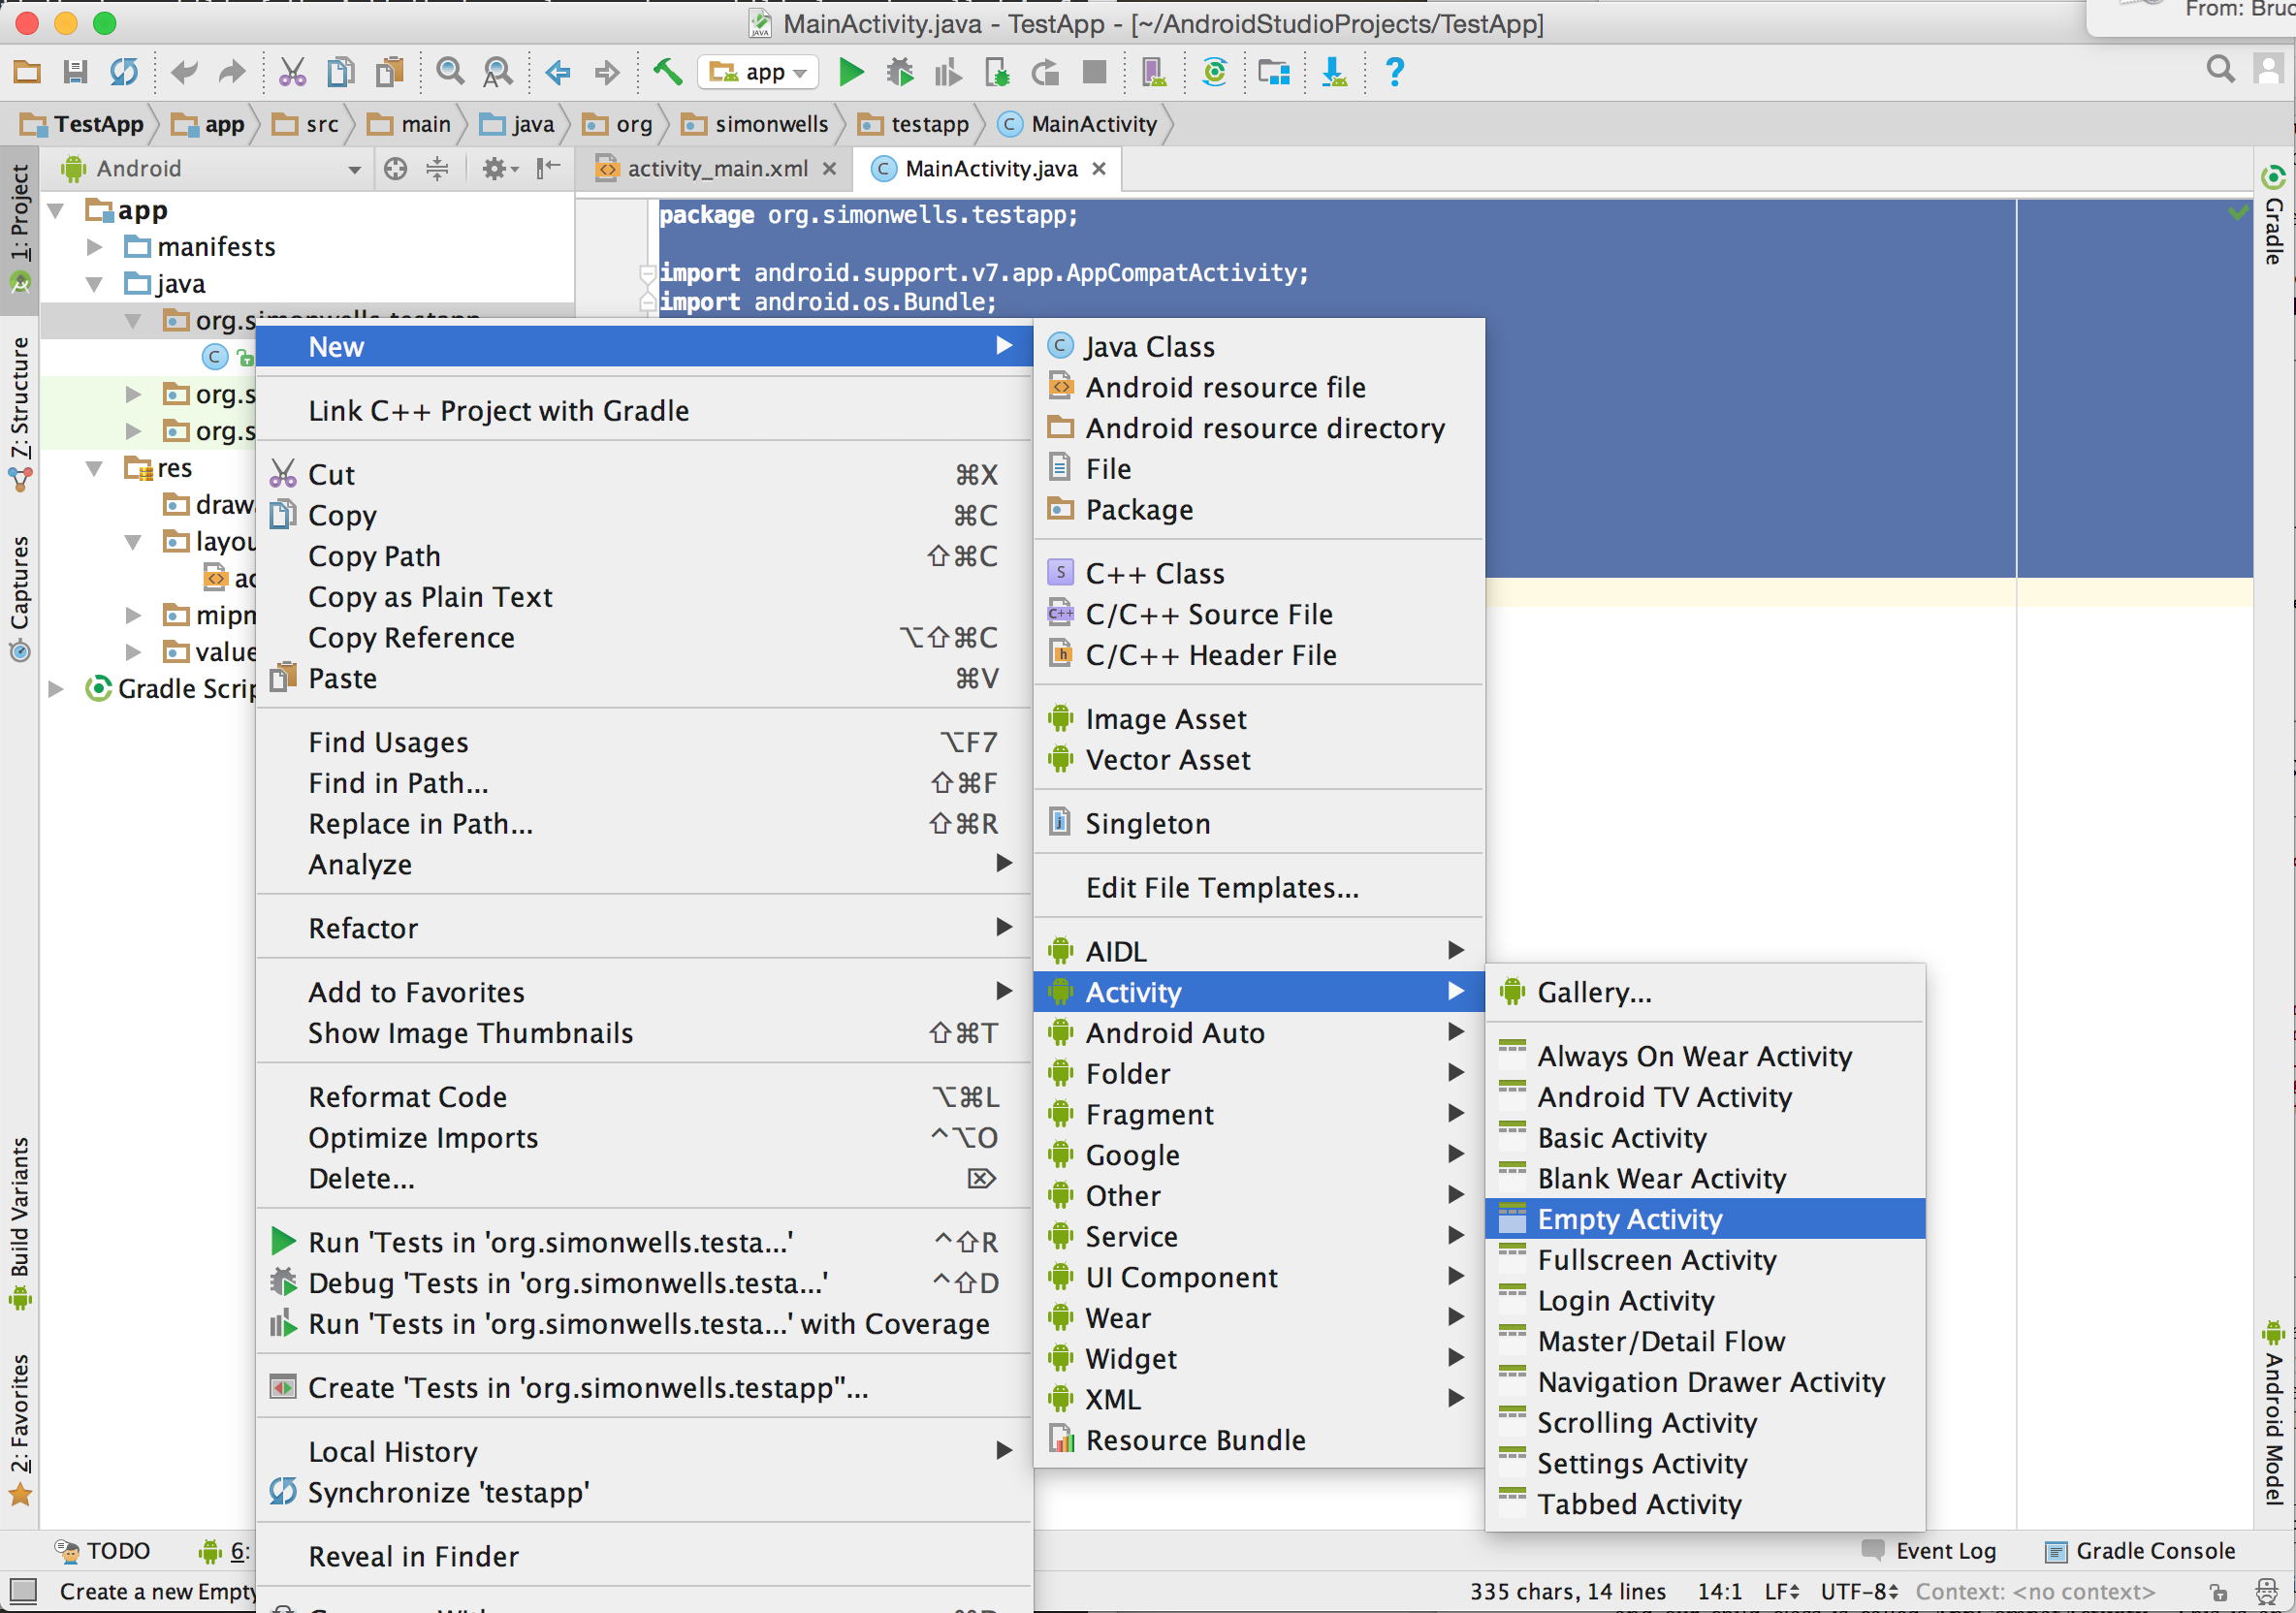
\includegraphics[width=\textwidth]{images/activities_add_activity_studio}
\caption{Android Studio Add Activity Options}
\label{fig:activities_add_activity_studio}
\end{figure}


\paragraph{} The new files that are generated for you include a java src file called `Main2Activity.java', an XML activity file called `activity\_main2.xml', and an entry in the AndroidManifest.xml file. Our project layout should now look something like the following:

\begin{figure}[H]
\centering
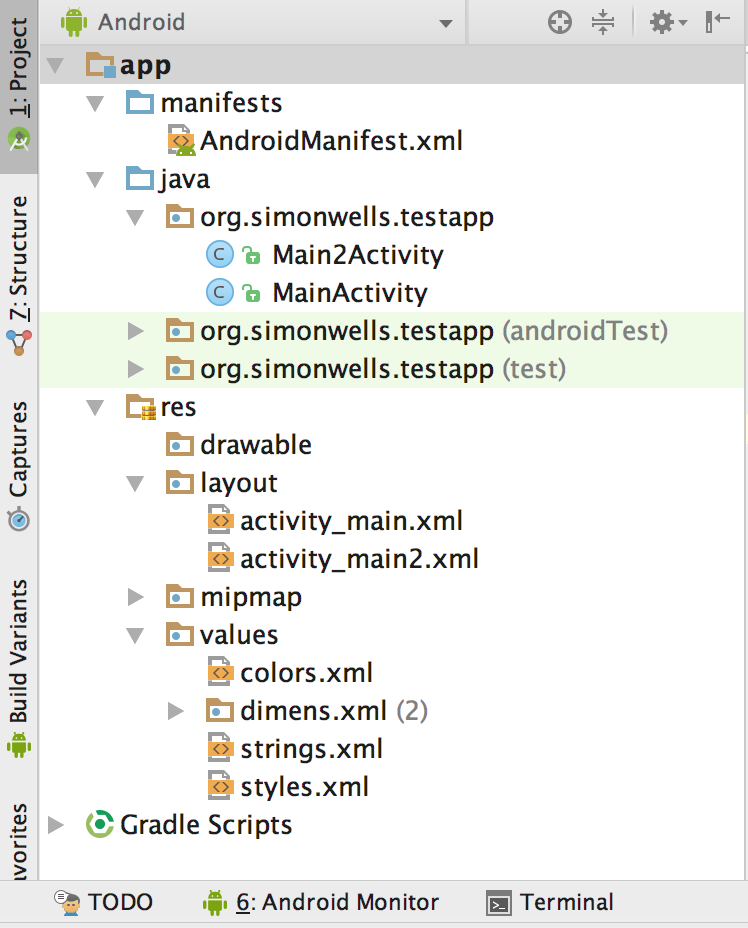
\includegraphics[width=\textwidth]{images/activities_project_explorer}
\caption{Android Project Files}
\label{fig:activities_project_explorer}
\end{figure}

\paragraph{} Notice that we have new Java and resource files for our new activity. Open up these files and explore tham. Compare the new activity files to the ones we started with. Other than different names, there should not be too much difference between them.

\paragraph{} There shouldn't be any real surprises in the MainActivity2.java file but if you are unsure, compare it to MainActivity.java

\begin{lstlisting}
package org.simonwells.testapp;

import android.support.v7.app.AppCompatActivity;
import android.os.Bundle;

public class Main2Activity extends AppCompatActivity {

    @Override
    protected void onCreate(Bundle savedInstanceState) {
        super.onCreate(savedInstanceState);
        setContentView(R.layout.activity_main2);
    }
}
\end{lstlisting}

\paragraph{} The layout for activity\_main2.xml looks pretty similar to activity\_main.xml

\begin{lstlisting}
<?xml version="1.0" encoding="utf-8"?>
<RelativeLayout xmlns:android="http://schemas.android.com/apk/res/android"
    xmlns:tools="http://schemas.android.com/tools"
    android:id="@+id/activity_main2"
    android:layout_width="match_parent"
    android:layout_height="match_parent"
    android:paddingBottom="@dimen/activity_vertical_margin"
    android:paddingLeft="@dimen/activity_horizontal_margin"
    android:paddingRight="@dimen/activity_horizontal_margin"
    android:paddingTop="@dimen/activity_vertical_margin"
    tools:context="org.simonwells.testapp.Main2Activity">

</RelativeLayout>

\end{lstlisting}

\paragraph{} As well as generating new files, Android Studio add a Manifest entry for the new Activity as shown here:

\begin{lstlisting}
<?xml version="1.0" encoding="utf-8"?>
<manifest xmlns:android="http://schemas.android.com/apk/res/android"
    package="org.simonwells.testapp">

    <application
        android:allowBackup="true"
        android:icon="@mipmap/ic_launcher"
        android:label="@string/app_name"
        android:supportsRtl="true"
        android:theme="@style/AppTheme">
        <activity android:name=".MainActivity">
            <intent-filter>
                <action android:name="android.intent.action.MAIN" />

                <category android:name="android.intent.category.LAUNCHER" />
            </intent-filter>
        </activity>
        <activity android:name=".Main2Activity"></activity>
    </application>

</manifest>
\end{lstlisting}


\paragraph{} That is all that is needed to create a new Activity as far as Android is concerned. Basically, two new files, a Java source file and an XML layout file, plus a couple of edits to the Android Manifest to make sure that your app knows about the new stuff. You can now run your app.

\paragraph{} Hmmm. Not much difference there? Why do you think that is?

\subsubsection{Switching Activities using the Android Manifest}

\paragraph{} The quickest way to display your new Activity is to edit the AndroidManifest.xml to tell it to launch the new activity instead of the default. Let's do that. All we need to do is move the $<$intent-filter$>$ block from MainActivity to our new MainActivity2 block as follows
\begin{lstlisting}
<?xml version="1.0" encoding="utf-8"?>
<manifest xmlns:android="http://schemas.android.com/apk/res/android"
    package="org.simonwells.testapp">

    <application
        android:allowBackup="true"
        android:icon="@mipmap/ic_launcher"
        android:label="@string/app_name"
        android:supportsRtl="true"
        android:theme="@style/AppTheme">
        <activity android:name=".MainActivity"></activity>
        <activity android:name=".Main2Activity">
            <intent-filter>
                <action android:name="android.intent.action.MAIN" />

                <category android:name="android.intent.category.LAUNCHER" />
            </intent-filter>
        </activity>
    </application>

</manifest>
\end{lstlisting}

\paragraph{} So your edited AndroidManifest.xml should look like this:

\paragraph{} Now run your app. You should now see the second Activity displayed. You can tell the difference because your second activity doesn't have the hello world message. Try adding some new elements to your Activities so that you can tell them apart more easily.

\paragraph{} But this isn't really good enough. We can't edit the app's manifest file every time we want to create a new Activity. We need another approach.

\subsubsection{Launching a new Activity from code}
\paragraph{} Create a new Android Studio project and add a second activity as we did earlier in the chapter. Once you know that it compiles and runs correctly you can do the following: Add a button to activity\_main.xml then add a handler for the button to your MainActivity.java file so that it looks like the following:

\begin{lstlisting}
package org.simonwells.testapp;

import android.content.Intent;
import android.support.v7.app.AppCompatActivity;
import android.os.Bundle;
import android.view.View;
import android.widget.Button;

public class MainActivity extends AppCompatActivity {

    @Override
    protected void onCreate(Bundle savedInstanceState) {
        super.onCreate(savedInstanceState);
        setContentView(R.layout.activity_main);

        Button btn = (Button) findViewById(R.id.button);
        btn.setOnClickListener(new View.OnClickListener() {
            @Override
            public void onClick(View view) {
                Intent activity2 = new Intent(MainActivity.this, Main2Activity.class);
                startActivity(activity2);
            }
        });
    }
}
\end{lstlisting}

\paragraph{} and your corresponding activity\_main.xml will look like this:

\begin{lstlisting}
<?xml version="1.0" encoding="utf-8"?>
<RelativeLayout xmlns:android="http://schemas.android.com/apk/res/android"
    xmlns:tools="http://schemas.android.com/tools"
    android:id="@+id/activity_main"
    android:layout_width="match_parent"
    android:layout_height="match_parent"
    android:paddingBottom="@dimen/activity_vertical_margin"
    android:paddingLeft="@dimen/activity_horizontal_margin"
    android:paddingRight="@dimen/activity_horizontal_margin"
    android:paddingTop="@dimen/activity_vertical_margin"
    tools:context="org.simonwells.testapp.MainActivity">

    <TextView
        android:layout_width="wrap_content"
        android:layout_height="wrap_content"
        android:text="Hello World!"
        android:id="@+id/textView" />

    <Button
        android:text="Button"
        android:layout_width="wrap_content"
        android:layout_height="wrap_content"
        android:layout_below="@+id/textView"
        android:layout_centerHorizontal="true"
        android:layout_marginTop="170dp"
        android:id="@+id/button" />
</RelativeLayout>

\end{lstlisting}

\paragraph{} Now run your app. You should be able to click the button and cause the second activity to be displayed. You will have to use the device's back button to return to the previous Activity. Consider how you might return to the previous activity from within your app? Perhaps a button or other navigation element that, when clicked finishes the current Activity and returns you to the parent? Do some research and see if you can work out how to do this for yourself.


%\subsection{Managing Multiple Activities}
%\paragraph{} Rather than creating a new activity for every screen in your app, it make sense to reuse resources when appropriate. For example, if your user is presented with a list of items that can be displayed, you could either have an activity for each item and switch between them after user interaction, or a single activity, designed to display your items consistently, which is reused based on user interaction. Having less activities, but reusing them in a sensible manner can help to stop your app from becoming unmanageable.


%\section{ViewGroups \& Layouts}
%\paragraph{}


\section{Some User Input}
\paragraph{} Remember, views are widgets that have an appearance onscreen. So user input widgets, such as text inputs, can use views just as output does. Let's explore some user input.

\paragraph{} Create a new project and check that it runs properly. Now delete the Hello World TextView so that we have an empty layout to play with.

\paragraph{} Add a ScrollView such as the following to your layout:

\begin{lstlisting}
<ScrollView
        android:layout_width="wrap_content"
        android:layout_height="wrap_content"
        android:id="@+id/scrollView"
        android:layout_centerVertical="true"
        android:layout_alignParentLeft="true"
        android:layout_alignParentStart="true"
        android:layout_marginLeft="42dp"
        android:layout_marginStart="42dp" >

        </ScrollView>
\end{lstlisting}

\paragraph{} Your activity\_main.xml should look similar to the following:

\begin{lstlisting}
<RelativeLayout xmlns:android="http://schemas.android.com/apk/res/android"
    xmlns:tools="http://schemas.android.com/tools" android:layout_width="match_parent"
    android:layout_height="match_parent" android:paddingLeft="@dimen/activity_horizontal_margin"
    android:paddingRight="@dimen/activity_horizontal_margin"
    android:paddingTop="@dimen/activity_vertical_margin"
    android:paddingBottom="@dimen/activity_vertical_margin" tools:context=".MainActivity">

    <ScrollView
        android:layout_width="wrap_content"
        android:layout_height="wrap_content"
        android:id="@+id/scrollView"
        android:layout_centerVertical="true"
        android:layout_alignParentLeft="true"
        android:layout_alignParentStart="true"
        android:layout_marginLeft="42dp"
        android:layout_marginStart="42dp" >
         
    </ScrollView>

</RelativeLayout>
\end{lstlisting}
\paragraph{} Don't worry if everything isn't \emph{exactly} the same. The graphical editor in Android Studio will sometimes try to be helpful and add extra parameters to give you a better layout.

\paragraph{} Now add a LinearLayout as a child of the ScrollView:

\begin{lstlisting}
<LinearLayout
            android:orientation="vertical"
            android:layout_width="fill_parent"
            android:layout_height="fill_parent"
            android:layout_below="@+id/scrollView"
            android:layout_centerHorizontal="true">
</LinearLayout>
\end{lstlisting}

\paragraph{} So you should end up with something like the following:

\begin{lstlisting}
<RelativeLayout xmlns:android="http://schemas.android.com/apk/res/android"
    xmlns:tools="http://schemas.android.com/tools" android:layout_width="match_parent"
    android:layout_height="match_parent" android:paddingLeft="@dimen/activity_horizontal_margin"
    android:paddingRight="@dimen/activity_horizontal_margin"
    android:paddingTop="@dimen/activity_vertical_margin"
    android:paddingBottom="@dimen/activity_vertical_margin" tools:context=".MainActivity">

    <ScrollView
        android:layout_width="wrap_content"
        android:layout_height="wrap_content"
        android:id="@+id/scrollView"
        android:layout_centerVertical="true"
        android:layout_alignParentLeft="true"
        android:layout_alignParentStart="true"
        android:layout_marginLeft="42dp"
        android:layout_marginStart="42dp" >

        <LinearLayout
            android:orientation="vertical"
            android:layout_width="fill_parent"
            android:layout_height="fill_parent"
            android:layout_below="@+id/scrollView"
            android:layout_centerHorizontal="true">

        </LinearLayout>

    </ScrollView>

</RelativeLayout>
\end{lstlisting}

\paragraph{} Neither of these elements, the ScrollView or LinearLayout do much visually. If you run the app now there isn't much to see. But they are containers which will help us to have a nice screen when we add the views in a few moments. For now, notice how the pair of $<$LinearLayout$>$ $<$/LinearLayout$>$ tags are children of, or come between, the $<$ScrollView$>$ $<$/ScrollView$>$ tags. We will deal with Layouts more in next weeks practical but for now just think of them as containers that holds views for you and automatically arrange them for you. All the ScrollView does is make its child view scrollable when the view won't fit on screen. A ScrollView can only have one child, which is our LinearLayout, but the child of the ScrollView can contain multiple further views. Lets try that out.

\paragraph{} Add three TextViews and three EditTexts to your layout so that you have three pairs of TextView then EditText, e.g. TextView, EditView, TextView, EditView, TextView, EditView in a column down the screen. Make sure to give each TextView and EditView an id so that you can reference each individually.Add strings for your TextViews to display so that the first TextView is the user's name, second is email address, and third is password.

\paragraph{} Your layout should now look similar to this:

\begin{lstlisting}
<RelativeLayout xmlns:android="http://schemas.android.com/apk/res/android"
    xmlns:tools="http://schemas.android.com/tools" android:layout_width="match_parent"
    android:layout_height="match_parent" android:paddingLeft="@dimen/activity_horizontal_margin"
    android:paddingRight="@dimen/activity_horizontal_margin"
    android:paddingTop="@dimen/activity_vertical_margin"
    android:paddingBottom="@dimen/activity_vertical_margin" tools:context=".MainActivity">

    <ScrollView
        android:layout_width="wrap_content"
        android:layout_height="wrap_content"
        android:id="@+id/scrollView"
        android:layout_centerVertical="true"
        android:layout_alignParentLeft="true"
        android:layout_alignParentStart="true"
        android:layout_marginLeft="42dp"
        android:layout_marginStart="42dp" >

        <LinearLayout
            android:orientation="vertical"
            android:layout_width="fill_parent"
            android:layout_height="fill_parent"
            android:layout_below="@+id/scrollView"
            android:layout_centerHorizontal="true">

            <TextView
                android:layout_width="wrap_content"
                android:layout_height="wrap_content"
                android:textAppearance="?android:attr/textAppearanceLarge"
                android:text="@string/name"
                android:id="@+id/tv1" />

            <EditText
                android:layout_width="match_parent"
                android:layout_height="wrap_content"
                android:id="@+id/et1"
                 />

            <TextView
                android:layout_width="wrap_content"
                android:layout_height="wrap_content"
                android:textAppearance="?android:attr/textAppearanceLarge"
                android:text="@string/email"
                android:id="@+id/tv2"
                 />

            <EditText
                android:layout_width="match_parent"
                android:layout_height="wrap_content"
                android:id="@+id/et2"
                android:inputType="textEmailAddress"
                 />

            <TextView
                android:layout_width="wrap_content"
                android:layout_height="wrap_content"
                android:textAppearance="?android:attr/textAppearanceLarge"
                android:text="@string/pw"
                android:id="@+id/tv3"
                 />

            <EditText
                android:layout_width="match_parent"
                android:layout_height="wrap_content"
                android:id="@+id/et3"
                android:password="true" />

        </LinearLayout>

    </ScrollView>

</RelativeLayout>

\end{lstlisting}

\paragraph{} Your strings.xml should look similar to this:

\begin{lstlisting}
<?xml version="1.0" encoding="utf-8"?>
<resources>

    <string name="app_name">UserInput</string>
    <string name="hello_world">Hello world!!!!</string>
    <string name="action_settings">Settings</string>
    <string name="name">Name</string>
    <string name="email">Email Address</string>
    <string name="pw">Password</string>

</resources>
\end{lstlisting}

\paragraph{} All other files in your project should be unchanged for now as we have only edited the layour and strings files, so try running your app now. You might want to futher adjust how things look. It is worth taking the time to do that now as this builds your experience of how Android apps work. When you run the app you should be able to input text into the three EditTexts. The password field should hide letters as you type them in. This behaviour is controlled by the following parameter of the EditText: 

\begin{lstlisting}
android:password="true"
\end{lstlisting}

\paragraph{} You should experiment with the other parameters that EditText, and other views have as you explore the Android platform features.

\paragraph{} Now lets consider doing something with the text entered into the EditText fields. Lets add some features to ensure that the name field is limited to a set number of characters in length and only allows names in upper-case. Open MainActivity.java and add the following code to the OnCreate method after the call to setContentView():

\begin{lstlisting}
    EditText nameTxt = (EditText) findViewById(R.id.et1);
    nameTxt.setFilters(new InputFilter[] {
        new InputFilter.LengthFilter(10),
        new InputFilter.AllCaps()
    });
\end{lstlisting}

\paragraph{} All this is doing is creating a variable, called nameTxt, that is associated with the EditText names et1. We have then used some built in classes to set some filters on the EditText, one of which limits the length of input to 10 chars, and the other which enforces upper-case. Run your app and try it out.

\paragraph{} Now lets do somethings a bit more advanced. Lets check the content of the supplied password to see whether it passes muster. For example, lets assume that the supplied password must contain a mixture of letters and numbers. A simple way to do this is to add a button which, when clicked, will take the text in the password field and tell us whether it is valid. So, add a button to your layout, inside the LinearLayout and after the last EditText:

\begin{lstlisting}
<Button
        android:layout_width="wrap_content"
        android:layout_height="wrap_content"
        android:text="@string/go"
        android:id="@+id/btn1"
        android:layout_below="@+id/scrollView"
        android:layout_centerHorizontal="true" />
\end{lstlisting}

\paragraph{} and add its content to the strings.xml e.g.

\begin{lstlisting}
<string name="go">GO!</string>
\end{lstlisting}

\paragraph{} You can run your app now and the button will be visible but it won't do anything because we haven't given it a handler to response to click events. So lets do that, add the following code to the OnCreate method of MainActivity.java after your code that added the input filters to the name field.

\begin{lstlisting}
final EditText pwfield = (EditText) findViewById(R.id.et3);
    Button go_button = (Button) findViewById(R.id.btn1);
    go_button.setOnClickListener(new View.OnClickListener() {
        @Override
        public void onClick(View v) {
            String text = pwfield.getText().toString();

            boolean valid = true;
            boolean hasNumbers = false;
            boolean hasLetters = false;

            for (int i=0; i<text.length(); i++) {
                char x = text.charAt(i);
                if (Character.isDigit(x)){
                    hasNumbers = true;
                }
                else if (Character.isLetter(x)) {
                    hasLetters = true;
                }
                else {
                    valid = false;
                    break;
                }
                if (valid && hasLetters && hasNumbers) {
                    Toast.makeText(getBaseContext(), "Password " + text + " is valid.", Toast.LENGTH_SHORT).show();
                }
                else {
                    Toast.makeText(getBaseContext(), "Password " + text + " is not valid.", Toast.LENGTH_SHORT).show();
                }

            }
        }

    });
\end{lstlisting}

\paragraph{} Most of this is normal Java. You should try to read the code to ensure that you understand exactly what is happening and why.

\paragraph{FURTHER EXERCISE} Try to add a handler for the email field which ensure that the supplied email address is correctly formatted. If you are unsure what constitutes a valid email address then it might be worth finding out more\footnote{\begin{itemize}\item Wikipedia Email Address Page: \url{http://en.wikipedia.org/wiki/Email_address} \item RFC5321 \url{http://tools.ietf.org/html/rfc5321} \item StackOverlfow discussion: \url{http://stackoverflow.com/questions/6119722/how-to-check-edittexts-text-is-email-address-or-not}\end{itemize}}.


\section{Summary}
\paragraph{} In this practical we have 

\begin{itemize}
\item Learnt about Activities
\item Worked with user input
\end{itemize}


\chapter{Layouts \& Visual Design}
\section{Aims}
\paragraph{} At the end of the practical portion of this topic you will be able to:

\begin{itemize}
\item Use layouts to manage the visual organisation of your views
%\item Fragments
%\item Dialogs (using Fragments)
%\item Action Bar
%\item Orientation
\item Design an app using simple graphical tools
\end{itemize}


\begin{framed}
{\bf{NOTICE:}} In this lab we will be dealing a lot with Views, i.e. user interface elements. In Android Studio you have the option of using the graphical layout tool or editing the layout XML files directly. If you use the graphical tool then it might add extra stuff to your layout file as it attempts to ``help'' you. This is OK but might make things display a little peculiarly. You can always remove these extrabits by editing the XML directly within the file. Either way you should be checking what the graphical editor adds to the XML file so that you become familiar with the underlying source code.
\end{framed}

\begin{framed}
{\bf{NOTICE 2:}} Try to avoid copying and pasting code from the practical notes into your editor. You will learn less this way than you do by typing it in yourself. Typing in the code counts as practise. And practising {\bf{always}} makes you better at the thing you are doing.

Copying and pasting has some additional drawbacks: it might introduce subtle errors into your code from copied white space, you will lose formatting so it is harder to comprehend your code, and you will lose the use of the auto-complete feature which sometimes adds in code, such as import statements.
\end{framed}

\section{Android Layouts}
\paragraph{} A layout is a class that manages the way that child views appear on screen. Anything that is a view or inherits from the View class can be a child of a layout. Layouts also inherit from View so they can be nested within each other. We should take note that there are `layout files', the xml files that you find in the res/layout/ folder, e.g.

\begin{framed}
res/layout/activity\_main.xml
\end{framed}

\paragraph{} and there are also Layout Views, graphical elements that you can use within layout files to organise the user interface elements. In this practical we will be using both aspects of layouts. We will be editing layout files and adding Layout Views to them, as well as other kinds of view. However, we will not spend a lot of time building fully working apps. The aim of this part of the practical is to get a solid understanding of how the different Layouts affect the arrangement of views on screen, but we won't necessarily link the views up to Java code that does things with them That is left as an exercise for you, for example, when a button is displayed, cause it to write out a log line in logcat, or display a Toast, just so that you can get some more practise.

\paragraph{} Android includes a number of standard layouts:

\begin{itemize}
\item Frame Layout
\item Linear Layout (in Horizontal \& Vertical flavours)
\item Table Layout
\item Grid Layout
\item Relative Layout
\end{itemize}

\paragraph{} In this practical we will look at a selection of useful Layouts. So, let's get started.

\paragraph{} Create a new Android project and open the activity\_main.xml layout so that you can edit it. Delete the existing ``Hello World'' text view (by clicking on it and pressing backspace. Now add three buttons to the default RelativeLayout. You should end up with something similar to the following:

\begin{lstlisting}
<RelativeLayout xmlns:android="http://schemas.android.com/apk/res/android"
    xmlns:tools="http://schemas.android.com/tools" android:layout_width="match_parent"
    android:layout_height="match_parent" android:paddingLeft="@dimen/activity_horizontal_margin"
    android:paddingRight="@dimen/activity_horizontal_margin"
    android:paddingTop="@dimen/activity_vertical_margin"
    android:paddingBottom="@dimen/activity_vertical_margin" tools:context=".MainActivity">

    <Button
        android:layout_width="wrap_content"
        android:layout_height="wrap_content"
        android:text="New Button"
        android:id="@+id/button"
        android:layout_gravity="center_vertical" />

    <Button
        android:layout_width="wrap_content"
        android:layout_height="wrap_content"
        android:text="New Button"
        android:id="@+id/button2"
        android:layout_gravity="center_vertical" />

    <Button
        android:layout_width="wrap_content"
        android:layout_height="wrap_content"
        android:text="New Button"
        android:id="@+id/button3"
        android:layout_gravity="center_vertical" />

</RelativeLayout>
\end{lstlisting}
\paragraph{} That's not ideal is it? All the buttons are placed directly on top of each other. We could give each button a specific position, but this would need to be adjusted for different screen sizes, dimensions, and orientations. It is much better to get the Android framework to manage the layout for us (unless we have something extra special that we want to do that the Android layouts can't manage). So let's try out some Layouts....

\subsection{Linear Layout}
\paragraph{} Delete the three buttons from your activity\_main.xml. Add a Horizontal Linear Layout View to your layout file. You should end up with something like this:

\begin{lstlisting}
<RelativeLayout xmlns:android="http://schemas.android.com/apk/res/android"
    xmlns:tools="http://schemas.android.com/tools" android:layout_width="match_parent"
    android:layout_height="match_parent" android:paddingLeft="@dimen/activity_horizontal_margin"
    android:paddingRight="@dimen/activity_horizontal_margin"
    android:paddingTop="@dimen/activity_vertical_margin"
    android:paddingBottom="@dimen/activity_vertical_margin" tools:context=".MainActivity">


    <LinearLayout
        android:orientation="horizontal"
        android:layout_width="fill_parent"
        android:layout_height="fill_parent">
        
    </LinearLayout>
</RelativeLayout>
\end{lstlisting}
\paragraph{} If we run this then we won't actually see very much output as the Layout itself doesn't have any visible view components of its own to display on screen. So we need to add some children to it. Lets put those buttons back but this time as children of the LinearLayout. You should have something like the following:

\begin{lstlisting}
<RelativeLayout xmlns:android="http://schemas.android.com/apk/res/android"
    xmlns:tools="http://schemas.android.com/tools" android:layout_width="match_parent"
    android:layout_height="match_parent" android:paddingLeft="@dimen/activity_horizontal_margin"
    android:paddingRight="@dimen/activity_horizontal_margin"
    android:paddingTop="@dimen/activity_vertical_margin"
    android:paddingBottom="@dimen/activity_vertical_margin" tools:context=".MainActivity">

    <LinearLayout
        android:orientation="horizontal"
        android:layout_width="fill_parent"
        android:layout_height="fill_parent">


        <Button
            android:layout_width="wrap_content"
            android:layout_height="wrap_content"
            android:text="New Button"
            android:id="@+id/button"
            android:layout_gravity="center_vertical" />

        <Button
            android:layout_width="wrap_content"
            android:layout_height="wrap_content"
            android:text="New Button"
            android:id="@+id/button2"
            android:layout_gravity="center_vertical" />

        <Button
            android:layout_width="wrap_content"
            android:layout_height="wrap_content"
            android:text="New Button"
            android:id="@+id/button3"
            android:layout_gravity="center_vertical" />

    </LinearLayout>
</RelativeLayout>

\end{lstlisting}

\paragraph{} Now when you run your app you should see the buttons arranged in a horizontal line across the middle of your screen.

\paragraph{} Now change the orientation parameter of your LinearLayout to vertical so we can try out another orientation of the buttons. 

\begin{lstlisting}
        android:orientation="vertical"
\end{lstlisting}

\paragraph{} When you run the app now you should see that the arrangement of the buttons is in a vertical line but that they are in the top left corner. Let's neaten that up a little by adding a gravity parameter to out LinearLayout:

\begin{lstlisting}
        android:gravity="center"
\end{lstlisting}

\paragraph{} Your vertical buttons should now be centered nicely on screen.

\subsection{Table Layout}
\paragraph{} This is similar to working with a spreadsheet or HTML table. This layout uses TableRow views to organise your views. Create a new project and add a TableLayout to your activity\_main.xml so that you have the following:

\begin{lstlisting}
<RelativeLayout xmlns:android="http://schemas.android.com/apk/res/android"
    xmlns:tools="http://schemas.android.com/tools" android:layout_width="match_parent"
    android:layout_height="match_parent" android:paddingLeft="@dimen/activity_horizontal_margin"
    android:paddingRight="@dimen/activity_horizontal_margin"
    android:paddingTop="@dimen/activity_vertical_margin"
    android:paddingBottom="@dimen/activity_vertical_margin" tools:context=".MainActivity">

    <TableLayout
        android:layout_width="fill_parent"
        android:layout_height="fill_parent">

    </TableLayout>
</RelativeLayout>
\end{lstlisting}

\paragraph{} This gives us an empty TableLayout. We now have to populate the table layout with TableRows and those rows need to be populated with actual visible views. Let's do that now; we are going to add three TableRows. In the first cell of the first row we will have a `back' button. In the second cell of the second row we will have a TextView for the user's `First Name' and in the second cell of the second row an EditText. We will have a similar set up for the third row only this time the label for the TextView should be `Last Name'. Your code should look similar to this:

\begin{lstlisting}
<RelativeLayout xmlns:android="http://schemas.android.com/apk/res/android"
    xmlns:tools="http://schemas.android.com/tools" android:layout_width="match_parent"
    android:layout_height="match_parent" android:paddingLeft="@dimen/activity_horizontal_margin"
    android:paddingRight="@dimen/activity_horizontal_margin"
    android:paddingTop="@dimen/activity_vertical_margin"
    android:paddingBottom="@dimen/activity_vertical_margin" tools:context=".MainActivity">

    <TableLayout
        android:layout_width="fill_parent"
        android:layout_height="fill_parent">

        <TableRow>
            <Button
                android:id="@+id/backbutton"
                android:text="Back"
                android:layout_width="wrap_content"
                android:layout_height="wrap_content" />
        </TableRow>

        <TableRow>
            <TextView
                android:text="First Name"
                android:layout_width="wrap_content"
                android:layout_height="wrap_content"
                android:layout_column="1" />
            <EditText
                android:width="100px"
                android:layout_width="wrap_content"
                android:layout_height="wrap_content" />
        </TableRow>

        <TableRow>
            <TextView
                android:text="Last Name"
                android:layout_width="wrap_content"
                android:layout_height="wrap_content"
                android:layout_column="1" />
            <EditText
                android:width="100px"
                android:layout_width="wrap_content"
                android:layout_height="wrap_content" />
        </TableRow>

    </TableLayout>
</RelativeLayout>
\end{lstlisting}



\subsection{Relative Layout} 
\paragraph{} If you have built `HelloAndroid' then you have already used the relative layout as it is the default created by the new Android project wizard. Now lets delve a little deeper. Create a new project, open the layout and delete the `Hello World' TextView.

\paragraph{} Now add an EditText, two TextViews, and a Button to your relative layout. Give the EditText an id of ``@+id/name'' and a hint of ``Enter your name''. Give the first TextView an id of ``@+id/date'' and text containg your birthday. Give the second TextView an id of ``@+id/time'' and text of the current time. Finally give your button the text ``done''. Your code should look similar to the following:

\begin{lstlisting}
<RelativeLayout xmlns:android="http://schemas.android.com/apk/res/android"
    xmlns:tools="http://schemas.android.com/tools" android:layout_width="match_parent"
    android:layout_height="match_parent" android:paddingLeft="@dimen/activity_horizontal_margin"
    android:paddingRight="@dimen/activity_horizontal_margin"
    android:paddingTop="@dimen/activity_vertical_margin"
    android:paddingBottom="@dimen/activity_vertical_margin" tools:context=".MainActivity">

    <EditText
        android:id="@+id/name"
        android:layout_width="fill_parent"
        android:layout_height="wrap_content"
        android:hint="Enter your name" />
    <TextView
        android:id="@+id/date"
        android:layout_width="wrap_content"
        android:layout_height="wrap_content"
        android:text="05.02.2015"/>
    <TextView
        android:id="@id/time"
        android:layout_width="wrap_content"
        android:layout_height="wrap_content"
        android:text="13:01 PM"/>
    <Button
        android:layout_width="wrap_content"
        android:layout_height="wrap_content"
        android:text="Done" />

</RelativeLayout>
\end{lstlisting}

\paragraph{} Obviously if you run this, those views will all be placed on top of each other as we haven't told the RelativeLayout how to lay out the view \emph{relative} to each other.

\begin{framed}
Good practise would be to use the strings.xml to hold the values of your views, e.g. yourEditText, TextViews, and Button - but I have not done that here just to try to keep the example code as straighforward as possible.
\end{framed}

\paragraph{} I think we should have the EditText at the top of the screen, with the two text views aligned in a row immediately below it. We should then have the button positioned below the TextViews. So let's do it. We need to add some parameters to our views to tell them where they should be positioned relative to each other. Lets start with the EditText and work our way along:

\begin{description}
\item[EditText] This is the easiest, it is the first item to be placed and so doesn't need any extra parameters to describe its location relative to other views.
\item[TextView `date'] We want this view to be below the name view (our EditText). We want it to be aligned to the left of the parent view, and left relative to the other TextView `time' so it needs the following parameters:
    \begin{lstlisting}
        android:layout_below="@id/name"
        android:layout_alignParentLeft="true"
        android:layout_toLeftOf="@+id/times"
    \end{lstlisting}
\item[TextView `time'] We want this to be below the EditText and aligned to the right of the parent layout so we can use the following parameters:
    \begin{lstlisting}
        android:layout_below="@id/name"
        android:layout_alignParentRight="true"
    \end{lstlisting}
\item[Button] We want to position this below the TextViews and centered in the parent layout so can use the following parameters:
    \begin{lstlisting}
        android:layout_below="@id/time"
        android:layout_centerInParent="true"
    \end{lstlisting}
\end{description}

\paragraph{} As a result our layout file, activity\_main.xml should look something like this:

\begin{lstlisting}
<RelativeLayout xmlns:android="http://schemas.android.com/apk/res/android"
    xmlns:tools="http://schemas.android.com/tools" android:layout_width="match_parent"
    android:layout_height="match_parent" android:paddingLeft="@dimen/activity_horizontal_margin"
    android:paddingRight="@dimen/activity_horizontal_margin"
    android:paddingTop="@dimen/activity_vertical_margin"
    android:paddingBottom="@dimen/activity_vertical_margin" tools:context=".MainActivity">

    <EditText
        android:id="@+id/name"
        android:layout_width="fill_parent"
        android:layout_height="wrap_content"
        android:hint="Enter your name" />
    <TextView
        android:id="@+id/date"
        android:layout_width="wrap_content"
        android:layout_height="wrap_content"
        android:layout_below="@id/name"
        android:layout_alignParentLeft="true"
        android:layout_toLeftOf="@+id/time"
        android:text="05.02.2015"/>
    <TextView
        android:id="@+id/time"
        android:layout_width="wrap_content"
        android:layout_height="wrap_content"
        android:layout_below="@id/name"
        android:layout_alignParentRight="true"
        android:text="13:01 PM"/>
    <Button
        android:layout_width="wrap_content"
        android:layout_height="wrap_content"
        android:layout_below="@id/time"
        android:layout_centerInParent="true"
        android:text="Done" />

</RelativeLayout>
\end{lstlisting}

\paragraph{} You can use the ids of each view to follow the layout of each relative to an earlier view, e.g. @+id/date is laid out below @+id/name and to the left of @+id/time.

\paragraph{} As an exercise, write Java code to display respectively the current date and time automatically in the two TextViews. Add functionality so that on pressing the button a unique Toast message is create which combines the user's name with the date and time, e.g. ``Hello Selina Kyle, it is now 13:01PM on 05.02.2015''

\subsection{ListView}
\paragraph{} This is a view which groups items and displays them in a scrollable, vertical list. This is a really useful and common interaction pattern on Android so we should become familiar with it. However it is a little more complicated than using a basic Layout. So we will build a complete app that displays a scrollable ListView containing a list of colours of the rainbow. You can of course make a list of whichever items you want.

\paragraph{} Create a new Android project and delete the `Hello World' TextView. Now, in activity\_main.xml we need to add our ListView widget. We can do it like this:

\begin{lstlisting}
<?xml version="1.0" encoding="utf-8"?>
<RelativeLayout xmlns:android="http://schemas.android.com/apk/res/android"
    xmlns:tools="http://schemas.android.com/tools"
    android:id="@+id/activity_main"
    android:layout_width="match_parent"
    android:layout_height="match_parent"
    android:paddingBottom="@dimen/activity_vertical_margin"
    android:paddingLeft="@dimen/activity_horizontal_margin"
    android:paddingRight="@dimen/activity_horizontal_margin"
    android:paddingTop="@dimen/activity_vertical_margin"
    tools:context="org.simonwells.listview_example.MainActivity">

    <ListView
        android:id="@+id/colour_list"
        android:layout_width="match_parent"
        android:layout_height="wrap_content"
        android:layout_centerVertical="true"
        android:layout_centerHorizontal="true" />

</RelativeLayout>
\end{lstlisting}

\paragraph{} We now need to add a new layout XML file. Right click in the file explorer area of Android Studio and select New $>$ XML $>$ Layout XML File. We'll name it layout\_textview and make the root tag a TextView as illustrated in the following figure: 

\begin{figure}[H]
\centering
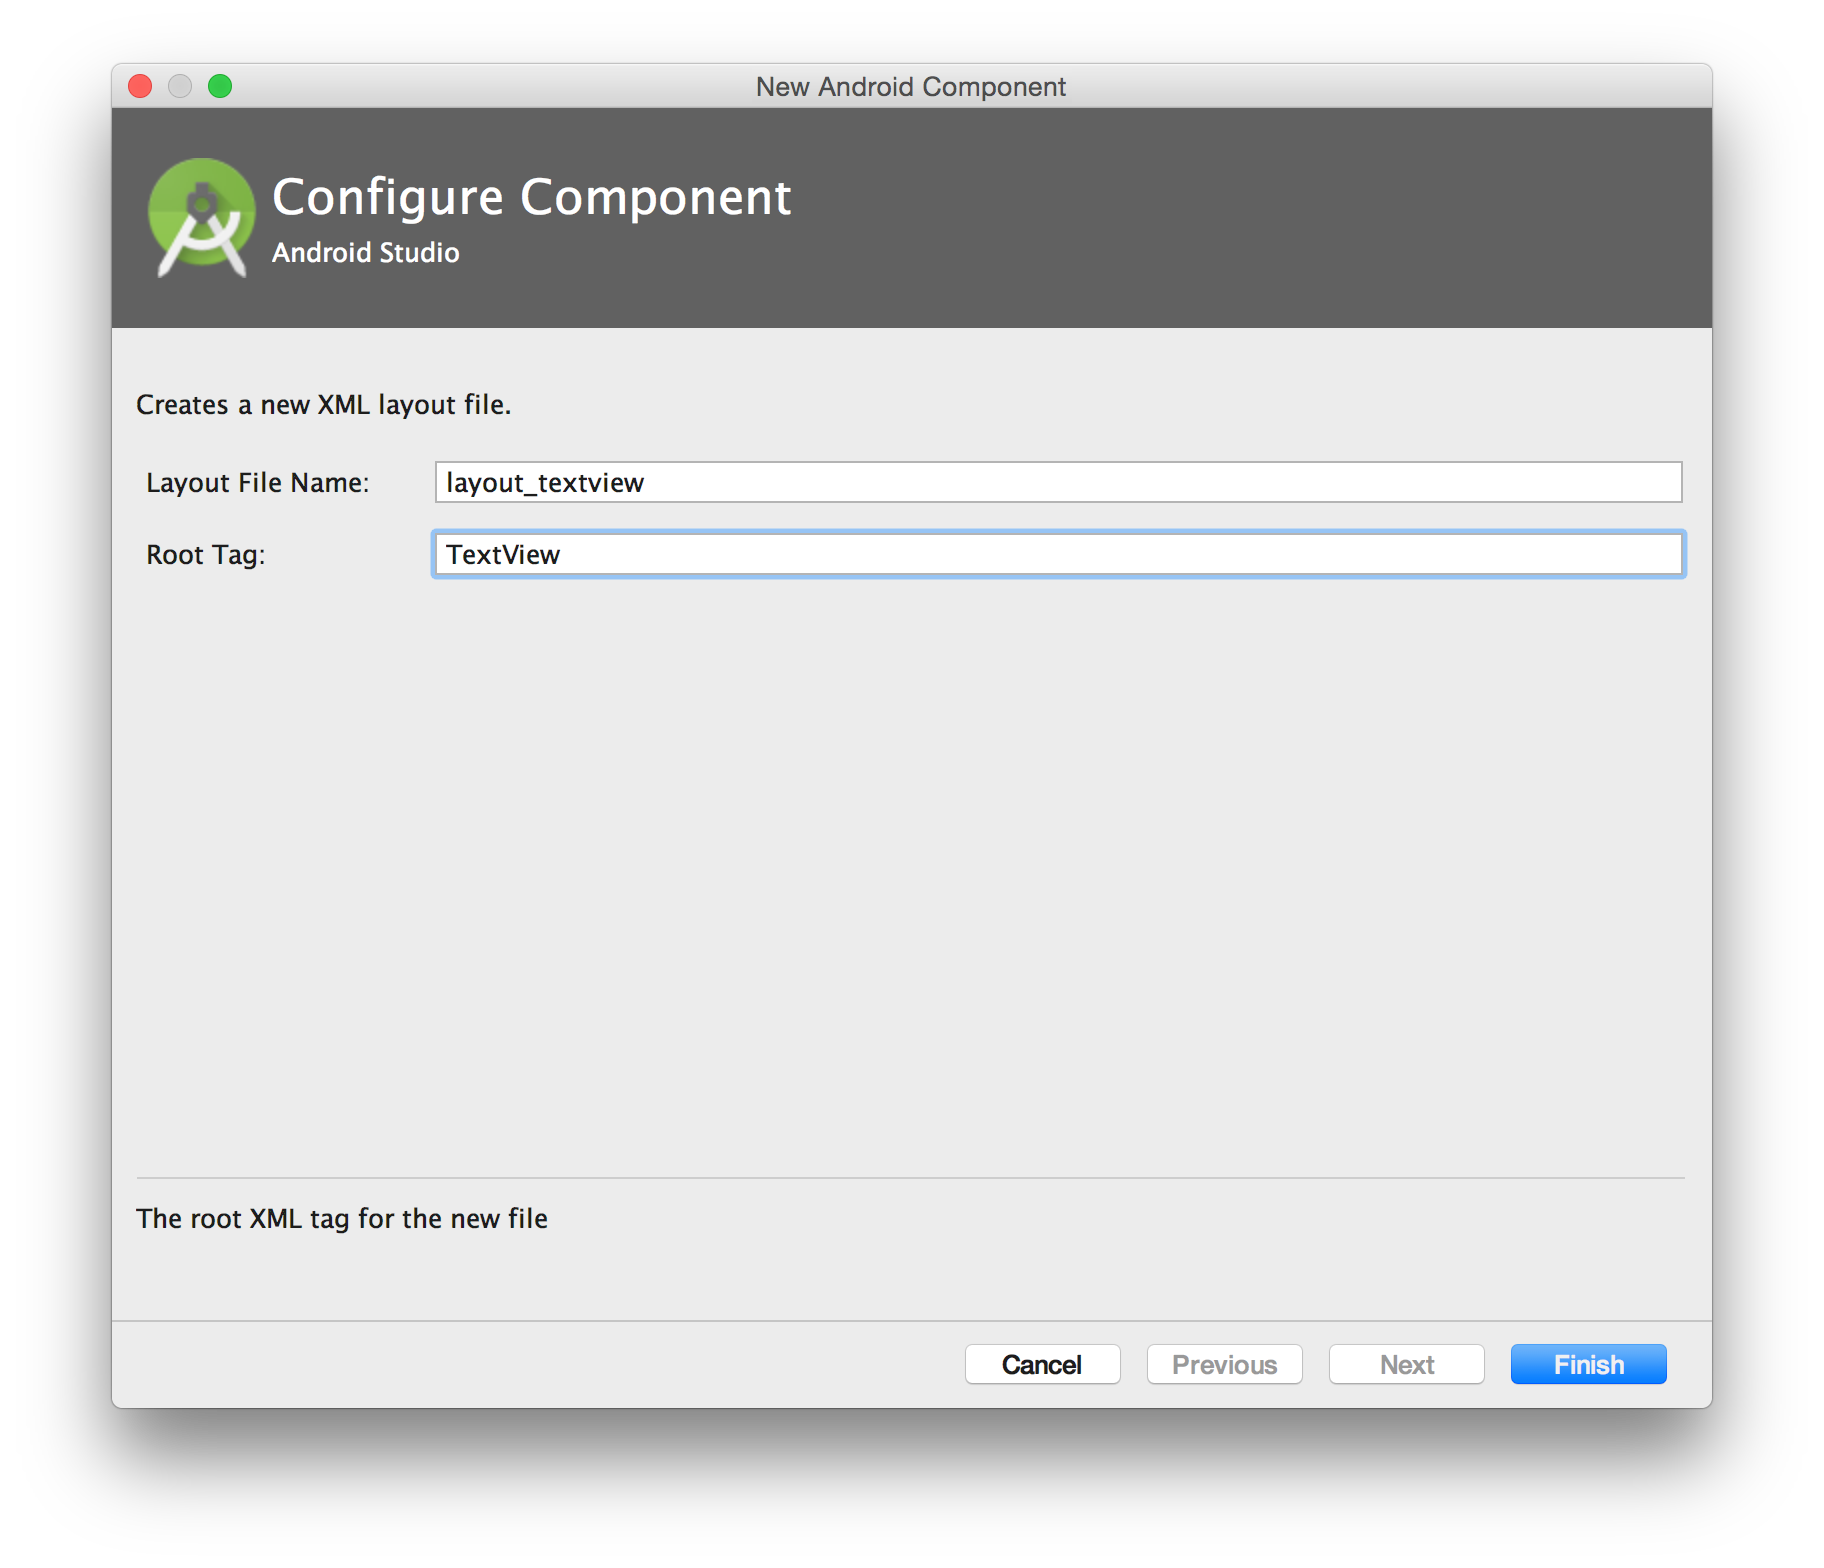
\includegraphics[width=\textwidth]{images/listview_layout_wizard}
\caption{Using the Android Studio wizard to add a new layout XML file}
\label{fig:listview_layout_wizard}
\end{figure}


Now edit layout\_textview as follows:

\begin{lstlisting}
<?xml version="1.0" encoding="utf-8"?>
<TextView xmlns:android="http://schemas.android.com/apk/res/android"
    android:id="@+id/label"
    android:layout_width="fill_parent"
    android:layout_height="fill_parent"
    android:padding="10dp"
    android:textSize="16dp"
    android:textStyle="bold" >
</TextView>
\end{lstlisting}

\paragraph{} This second layout is essentially just the content of each element of the listview that will be displayed. 

\paragraph{} Now finally, we can link all these bits together by editing MainActivity.java. We want to do two things. Firstly, populate the ListView, and secondly, react to clicks on the list by displaying a Toast of the list contents. Our MainActivity.java should look like this:

\begin{lstlisting}
package org.simonwells.listview_example;

import android.support.v7.app.AppCompatActivity;
import android.os.Bundle;
import android.view.View;
import android.widget.AdapterView;
import android.widget.ArrayAdapter;
import android.widget.ListView;
import android.widget.Toast;

public class MainActivity extends AppCompatActivity {

    String[] colourArray = {"Red", "Orange", "Yellow", "Green", "Blue", "Indigo", "Violet"};

    @Override
    protected void onCreate(Bundle savedInstanceState) {
        super.onCreate(savedInstanceState);
        setContentView(R.layout.activity_main);

        ArrayAdapter adapter = new ArrayAdapter<String>(this,
                R.layout.layout_textview, colourArray);
        final ListView listView = (ListView) findViewById(R.id.colour_list);
        listView.setAdapter(adapter);

        listView.setOnItemClickListener(new AdapterView.OnItemClickListener() {
            @Override
            public void onItemClick(AdapterView<?> adapterView, View view, int i, long l) {
                String selection = (String) (listView.getItemAtPosition(i));
                Toast.makeText(getApplicationContext(), selection, Toast.LENGTH_SHORT).show();
            }
        });
    }
}
\end{lstlisting}

\paragraph{} You can now run your app. Assuming that everything has right you should now be able to view a scrollable list of colours of the rainbow (or whatever else you put in the list).

\begin{figure}[H]
\centering
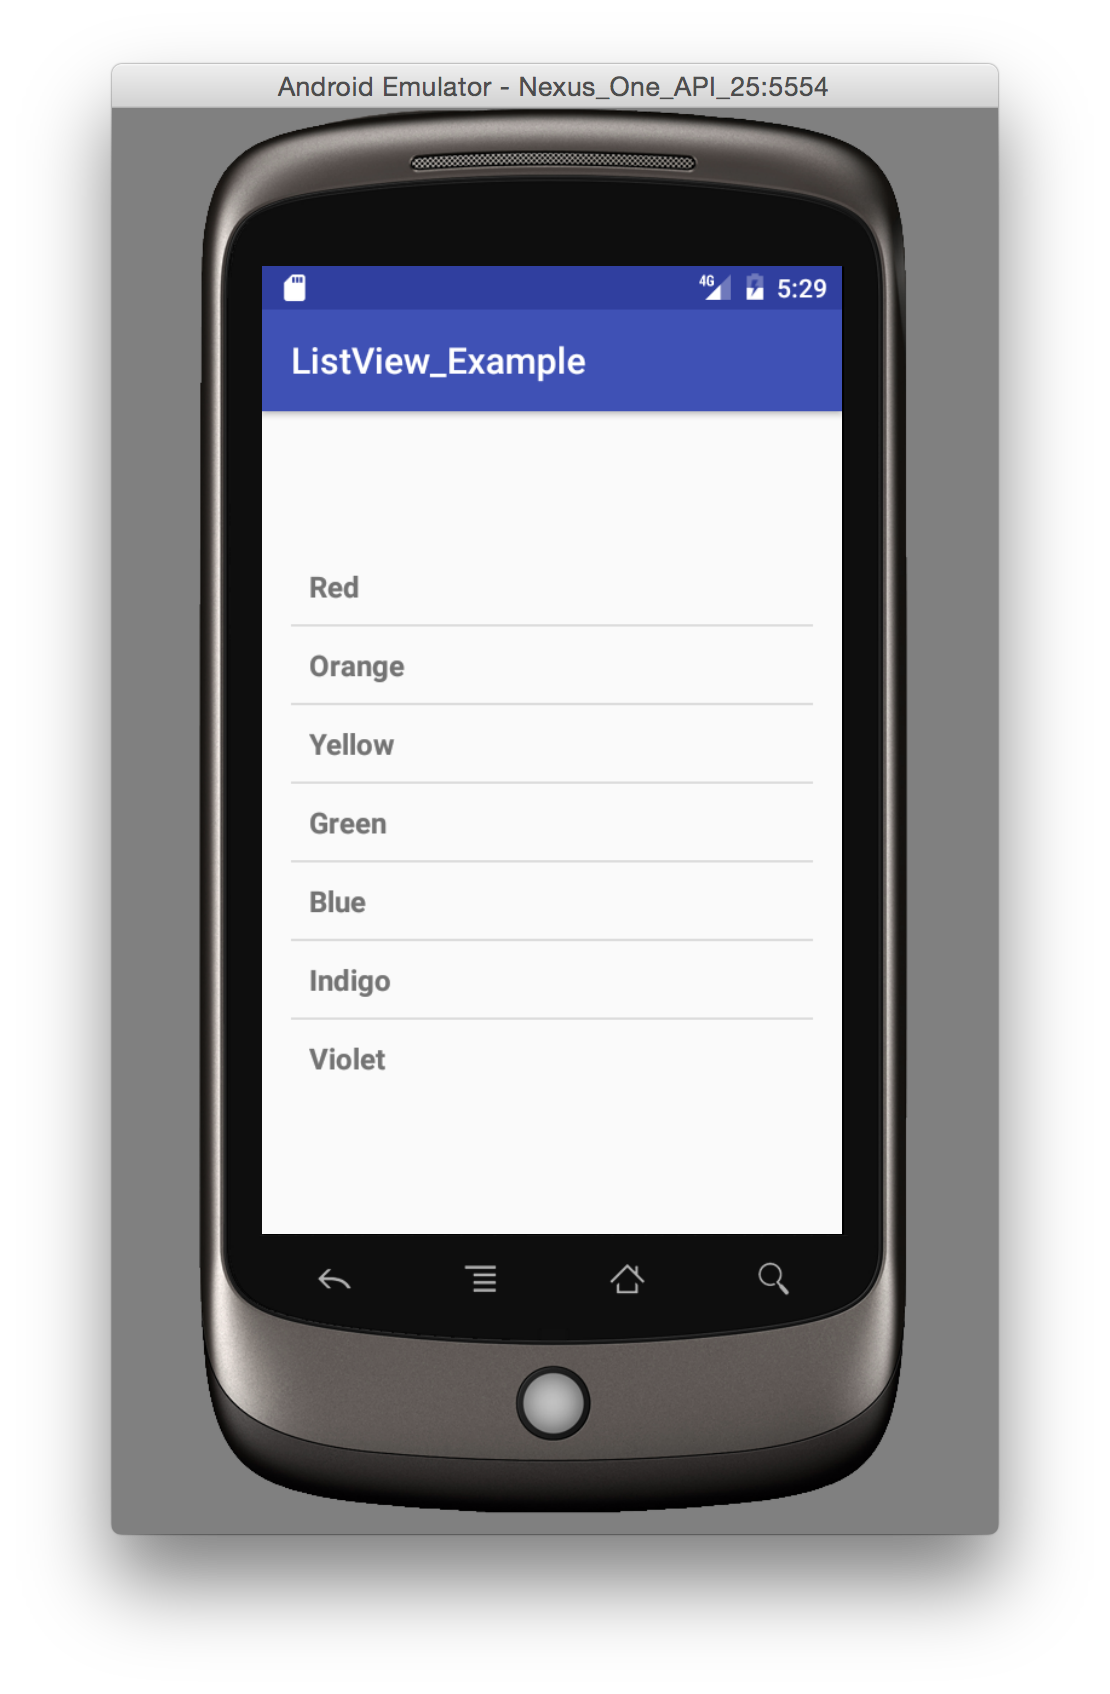
\includegraphics[width=0.8\textwidth]{images/listview_avd}
\caption{AVD showing the listview example app}
\label{fig:listview_avd}
\end{figure}


\paragraph{} We haven't gone into as much detail explaining what is happening in the ListView as in other examples. This is because it is mostly built from things we have already seen. It is a combination of basic views, layouts, and activities glued together with a bit of Java. Once you have it running you should spend some time getting an understanding of how it all fits together.

\paragraph{} In summary, layouts are a powerful and useful way to build flexible and dynamic layouts for your app and are, as a rule, much preferred over hard coding the layouts, especially when dealing with different screen sizes.



%\section{Dialogs (using Fragments)}
%\paragraph{} By default an activity occupies the entire screen. However you can apply a dialog theme so that your activity is displayed as a floating dialog which can sometime be useful to warn users or to double check that a user is sure of their action (when an action could have potentially bad consequences such as deleting data).

\section{Designing Apps}
\paragraph{} You shouldn’t spend months on your app before checking if the design will work. The use of storyboards and navigation maps followed by a rapid development application development tool will help you mock up a template to test your design early on and hopefully find any flaws with your design.

\paragraph{} We will design a home page (default activity displayed when an app is launched by clicking its icon) for an app. You can base this on your coursework idea (if you have one) or any other app that you would like to consider. If you don't have any ideas or want to try something different then perhaps design the home-page for a weather display app:

\begin{framed}
Assume that you have an API available which will allow your device to remotely retrieve information about the weather conditions and perhaps forecast for a named area, e.g. Edinbugh. You can use the data returned by the API of OpenWeathermap\footnote{\url{openweathermap.org}} as an exemplar of what data might be available to you. Design a home page to display this data, or a sensible subset, to your user.
\end{framed}

\begin{itemize}
\item Start will a storyboard for a layout, we will need a home page that will link to a photo gallery of attractions, a page that will link to various tourists sites and a page about our application itself.
\item Decide on a prototyping tool such as PhoneGap\footnote{\url{http://phonegap.com/}}, App Inventor\footnote{\url{http://appinventor.mit.edu/}}, using the XML layout designer in Android Studioor any other tool you feel comfortable using, NB. Try a search for ``Android Wireframe Mockup tools'' and you will be surprised by the number available\footnote{\url{http://mashable.com/2013/04/02/wireframing-tools-mobile/} is a good place to start}. If you are not sure where to start then try the XML Layout Designer of Android Studio as it is already installed in the labs. If you are still unsure there are plenty of comparison articles available online\footnote{\url{http://www.amlcode.com/2010/07/16/comparison-appinventor-rhomobile-phonegap-appcelerator-webview-and-aml/}}.
\item Try and develop the basic layout to the Weather App from above. Alternatively,  spend the time trying to prototype your own coursework app.
\end{itemize}

\section{Summary}
\paragraph{} In this practical we have: 

\begin{itemize}
\item Explored Android Layouts and Views for managing how your UI is displayed.
\item Begun prototyping Android apps using appropriate prototype and mockup tools.
\end{itemize}

\chapter{Persistence}
\section{Aims}
\paragraph{} At the end of the practical portion of this topic you will be able to:

\begin{itemize}
\item Use Shared Preferences to store basic Java datatypes in Key:Value format
\item Use Internal \& external storage to store files
\item Use SQLite to store data in Android's default DB system
\end{itemize}

\section{Shared Preferences}
\paragraph{} Shared preferences (accessed through the SharedPreferences class) are a dictionary of key-value pairs that can be used to store primitive Java data-types. This is most commonly used to store app and user settings and preferences or small amounts of simple data. 

\paragraph{} Using shared preferences to store small bits of data, confined to basic Java datatypes, is straightforward. Lets try it out now.  We are going to create an app that displays two buttons. One button will store some data, a randomly generated high score, in our shared preferences and the other button will read some data from our shared preferences. To keep things simple, feedback of what is read or written will be displayed after each button press using Toasts. This small app will illustrate how to store a single key and value into a specified shared preferences file. You should be able to build on this to incorporate simple data storage of Java datatypes into your app if appropriate.

\paragraph{} Create a new Android project and delete the `Hello World' label. Now open `strings.xml' and add some new strings. We need a string to store the name of the shared preferences file `preference\_file\_name' and a string for the name of our data key `high\_score'. We also need two more strings for the labels for our buttons, `get\_something' and `do\_something'. Our strings.xml should look similar to this:

\begin{lstlisting}
<resources>
    <string name="app_name">SharedPreferences</string>
    <string name="preference_file_name">MyPrefs</string>
    <string name="high_score">0</string>
    <string name="get_something">Get Prefs</string>
    <string name="do_something">Add Pref</string>
</resources>
\end{lstlisting}

\paragraph{} Now we can edit our layout to display the buttons. Edit your activity\_main.xml so that it uses a LinearLayout and give this layout two buttons, `btn1' and `btn2' as children. The text for `btn1' should use the `get\_something' string and the text for `btn2' should use the `do\_something' string that we just added to strings.xml. When you are done, your activity\_main.xml should look something like this:

\begin{lstlisting}
<?xml version="1.0" encoding="utf-8"?>
<LinearLayout xmlns:android="http://schemas.android.com/apk/res/android"
    xmlns:tools="http://schemas.android.com/tools"
    android:id="@+id/activity_main"
    android:layout_width="match_parent"
    android:layout_height="match_parent"
    android:paddingBottom="@dimen/activity_vertical_margin"
    android:paddingLeft="@dimen/activity_horizontal_margin"
    android:paddingRight="@dimen/activity_horizontal_margin"
    android:paddingTop="@dimen/activity_vertical_margin"
    android:orientation="vertical"
    tools:context="org.simonwells.sharedpreferences.MainActivity">

    <Button
        android:layout_width="wrap_content"
        android:layout_height="wrap_content"
        android:text="@string/get_something"
        android:id="@+id/btn1"
        android:layout_gravity="center_horizontal" />

    <Button
        android:layout_width="wrap_content"
        android:layout_height="wrap_content"
        android:text="@string/do_something"
        android:id="@+id/btn2"
        android:layout_gravity="center_horizontal" />

</LinearLayout>
\end{lstlisting}

\paragraph{} Ensure that your app compiles and runs before proceeding. If necessary, fix any bugs or typos as there's no point adding more code until what we have works. Our MainActivity.java file should end up looking something similar to the following:

\begin{lstlisting}
package org.simonwells.sharedpreferences;

import android.content.Context;
import android.content.SharedPreferences;
import android.support.v7.app.AppCompatActivity;
import android.os.Bundle;
import android.view.View;
import android.widget.Button;
import android.widget.Toast;

import java.util.Map;
import java.util.Random;

public class MainActivity extends AppCompatActivity {

    @Override
    protected void onCreate(Bundle savedInstanceState) {
        super.onCreate(savedInstanceState);
        setContentView(R.layout.activity_main);

        final Random rnd = new Random();

        Button get_something = (Button) findViewById(R.id.btn1);
        get_something.setOnClickListener(new View.OnClickListener() {
            @Override
            public void onClick(View view) {
                SharedPreferences prefs = getBaseContext().getSharedPreferences("MyPrefs", Context.MODE_PRIVATE);
                Map mp = prefs.getAll();
                Toast.makeText(getBaseContext(), mp.toString(), Toast.LENGTH_SHORT).show();
            }
        });

        Button do_something = (Button) findViewById(R.id.btn2);
        do_something.setOnClickListener(new View.OnClickListener() {
            @Override
            public void onClick(View view) {
                SharedPreferences prefs = getBaseContext().getSharedPreferences("MyPrefs", Context.MODE_PRIVATE);
                int newHighScore = rnd.nextInt(1000);
                SharedPreferences.Editor editor = prefs.edit();
                editor.putInt("0", newHighScore);
                editor.commit();
                Toast.makeText(getBaseContext(), "New High Score: "+newHighScore, Toast.LENGTH_SHORT).show();
            }
        });
    }
}
\end{lstlisting}

\paragraph{} Let's take a look at all the things that we just did:

\begin{enumerate}
\item Set up a random number object, e.g.
\begin{lstlisting}
    final Random rnd = new Random();
\end{lstlisting}
\item Create a button handler to retrieve all of the keys and values in the shared preference file as a map and display the contents of the map in a Toast.
\begin{lstlisting}
Button get_something = (Button) findViewById(R.id.btn1);
        get_something.setOnClickListener(new View.OnClickListener() {
            @Override
            public void onClick(View v) {
                SharedPreferences prefs = getBaseContext().getSharedPreferences(getString(R.string.preference_file_name), Context.MODE_PRIVATE);
                Map mp = prefs.getAll();
                Toast.makeText(getBaseContext(), mp.toString(), Toast.LENGTH_SHORT).show();
            }
        });
\end{lstlisting}
\item Create a button handler in which we edit our shared preference file to set a high score value, basically store an int that our random number object supplies.
\begin{lstlisting}
Button do_something = (Button) findViewById(R.id.btn2);
        do_something.setOnClickListener(new View.OnClickListener() {
            @Override
            public void onClick(View v) {
                SharedPreferences prefs = getBaseContext().getSharedPreferences(getString(R.string.preference_file_name), Context.MODE_PRIVATE);
                //Map mp = prefs.getAll();
                int newHighScore = rnd.nextInt(1000);
                SharedPreferences.Editor editor = prefs.edit();
                editor.putInt(getString(R.string.high_score), newHighScore);
                editor.commit();
                Toast.makeText(getBaseContext(), "New High Score"+newHighScore, Toast.LENGTH_SHORT).show();
            }
        });
\end{lstlisting}
\end{enumerate}


\paragraph{} When you run it, your new app should look something like the following:

\begin{figure}[H]
\centering
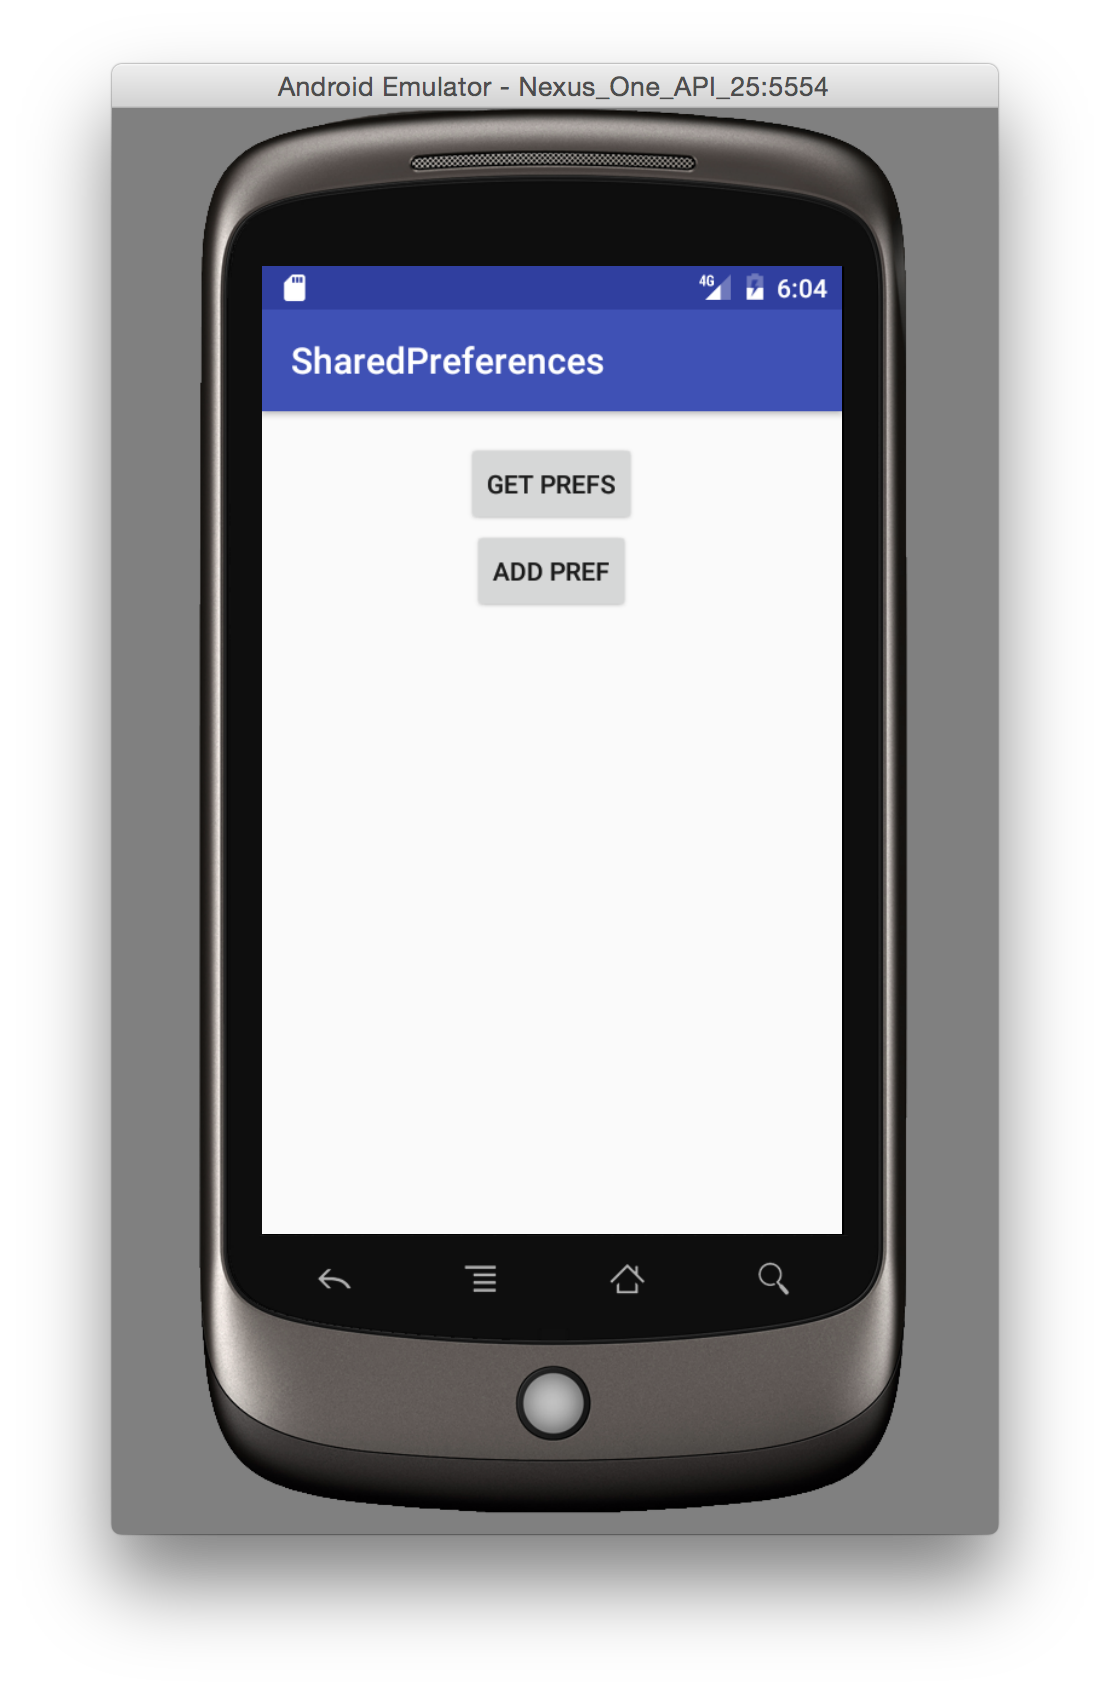
\includegraphics[width=0.8\textwidth]{images/sharedprefs_avd}
\caption{The Shared Prefs Example}
\label{fig:sharedprefs_avd}
\end{figure}

\paragraph{} You should use the Shared preferences documentation\footnote{\url{http://developer.android.com/reference/android/content/SharedPreferences.html}} to explore more functionality of this aspect of data storage. Try retrieving the specific key rather than all of the keys in the get\_something button handler. Now try storing your name into the shared preferenced file and retrieving it.

\paragraph{} Although you can exploit this for more advanced data storage requirements, the trouble and complexities of doing so can mean that it is better to adopt other strategies. The most appropriate storage method for a given app is highly dependent upon that app, what it is designed to do, and how that design is implemented.

\section{Internal Storage}
\paragraph{} Every app has a private directory, outside of the application bundle, in which it can store files. This is usually located on the devices internal storage and is private to the app and cannot be accessed by any other apps. These files are tied to the lifetime of the app and deleted when the app is deleted (but are kept during updates). The Android training documentation\footnote{\url{http://developer.android.com/training/basics/data-storage/files.html}} has more information on saving files to internal storage.

\paragraph{} For this part of the pracical we will build a similar interface to the one we did for the shared preferences data perisistence example earlier, e.g. a button to save some data to a file on internal storage and a button to load the data from that file and display the loaded data using a Toast. The data we will store will be the data as this is something that is straightforward to generate and is dynamic so will change the data stored each time we press the save button.

\paragraph{} Create a new Android project. Delete the `Hello World' TextView and add to buttons, `Save Something' and `load something' to a vertical LinearLayout. Add appropriate strings to support this to strings.xml so that your activity\_main.xml i something like the following:

\begin{lstlisting}
<RelativeLayout xmlns:android="http://schemas.android.com/apk/res/android"
    xmlns:tools="http://schemas.android.com/tools" android:layout_width="match_parent"
    android:layout_height="match_parent" android:paddingLeft="@dimen/activity_horizontal_margin"
    android:paddingRight="@dimen/activity_horizontal_margin"
    android:paddingTop="@dimen/activity_vertical_margin"
    android:paddingBottom="@dimen/activity_vertical_margin" tools:context=".MainActivity">

    <LinearLayout
        android:orientation="vertical"
        android:layout_width="fill_parent"
        android:layout_height="fill_parent"
        android:layout_centerVertical="true"
        android:layout_centerHorizontal="true">

        <Button
            android:layout_width="wrap_content"
            android:layout_height="wrap_content"
            android:text="@string/save_file"
            android:id="@+id/button1"
            android:layout_gravity="center_horizontal" />

        <Button
            android:layout_width="wrap_content"
            android:layout_height="wrap_content"
            android:text="@string/load_file"
            android:id="@+id/button2"
            android:layout_gravity="center_horizontal" />
    </LinearLayout>
</RelativeLayout>
\end{lstlisting}

\paragraph{} and your strings.xml is something like the following:

\begin{lstlisting}
<?xml version="1.0" encoding="utf-8"?>
<resources>

    <string name="app_name">TestInternalFile</string>
    <string name="hello_world">Hello world!</string>
    <string name="action_settings">Settings</string>
    <string name="load_file">LOAD SOMETHING</string>
    <string name="save_file">SAVE SOMETHING</string>

</resources>
\end{lstlisting}

\paragraph{} That gives us an interface with some buttons ready to do something. Now all we need to do is get the buttons to actually do something, like saving and loading files. To do this we need to add click listeners for each button to the onCreate method in MainActivity.java where the listener for the first button creates a new file, generates a string from the current date, then writes the string to the file we specified. For example, 

\begin{lstlisting}
Button btn1 = (Button) findViewById(R.id.button1);
        btn1.setOnClickListener(new View.OnClickListener() {
            @Override
            public void onClick(View v) {

                String filename = "napierfile";
                String outString = new Date().toString();
                FileOutputStream outStream;

                try {
                    outStream = getApplicationContext().openFileOutput(filename, Context.MODE_PRIVATE);
                    outStream.write(outString.getBytes());
                    outStream.close();
                } catch (Exception e) {
                    e.printStackTrace();
                }
            }
        });
\end{lstlisting}

\paragraph{} For our second button we want to read in the contents of our specified file then display those contents in a Toast. For example,

\begin{lstlisting}
Button btn2 = (Button) findViewById(R.id.button2);
        btn2.setOnClickListener(new View.OnClickListener() {
            @Override
            public void onClick(View v) {
                int ch;

                String filename = "napierfile";
                StringBuffer inString = new StringBuffer("");
                FileInputStream inStream;

                try {
                    inStream = getApplicationContext().openFileInput(filename);
                    try {
                        while ((ch = inStream.read()) != -1)
                            inString.append((char) ch);
                    } catch (IOException e) {
                        e.printStackTrace();
                    }
                    inStream.close();
                } catch (Exception e) {
                    e.printStackTrace();
                }

                String data = new String(inString);
                Toast.makeText(getBaseContext(),data,Toast.LENGTH_SHORT).show();
            }
        });
\end{lstlisting}

\paragraph{} Putting this all together, our MainActivity.java should look something similar to the following:

\begin{lstlisting}
package org.simonwells.testinternalfile;

import android.content.Context;
import android.support.v7.app.ActionBarActivity;
import android.os.Bundle;
import android.view.Menu;
import android.view.MenuItem;
import android.view.View;
import android.widget.Button;
import android.widget.Toast;

import java.io.FileInputStream;
import java.io.FileOutputStream;
import java.io.IOException;
import java.util.Date;


public class MainActivity extends ActionBarActivity {

    @Override
    protected void onCreate(Bundle savedInstanceState) {
        super.onCreate(savedInstanceState);
        setContentView(R.layout.activity_main);

        Button btn1 = (Button) findViewById(R.id.button1);
        btn1.setOnClickListener(new View.OnClickListener() {
            @Override
            public void onClick(View v) {

                String filename = "napierfile";
                String outString = new Date().toString();
                FileOutputStream outStream;

                try {
                    outStream = getApplicationContext().openFileOutput(filename, Context.MODE_PRIVATE);
                    outStream.write(outString.getBytes());
                    outStream.close();
                } catch (Exception e) {
                    e.printStackTrace();
                }
            }
        });

        Button btn2 = (Button) findViewById(R.id.button2);
        btn2.setOnClickListener(new View.OnClickListener() {
            @Override
            public void onClick(View v) {
                int ch;

                String filename = "napierfile";
                StringBuffer inString = new StringBuffer("");
                FileInputStream inStream;

                try {
                    inStream = getApplicationContext().openFileInput(filename);
                    try {
                        while ((ch = inStream.read()) != -1)
                            inString.append((char) ch);
                    } catch (IOException e) {
                        e.printStackTrace();
                    }
                    inStream.close();
                } catch (Exception e) {
                    e.printStackTrace();
                }

                String data = new String(inString);
                Toast.makeText(getBaseContext(),data,Toast.LENGTH_SHORT).show();
            }
        });
    }

    @Override
    public boolean onCreateOptionsMenu(Menu menu) {
        // Inflate the menu; this adds items to the action bar if it is present.
        getMenuInflater().inflate(R.menu.menu_main, menu);
        return true;
    }

    @Override
    public boolean onOptionsItemSelected(MenuItem item) {
        // Handle action bar item clicks here. The action bar will
        // automatically handle clicks on the Home/Up button, so long
        // as you specify a parent activity in AndroidManifest.xml.
        int id = item.getItemId();

        //noinspection SimplifiableIfStatement
        if (id == R.id.action_settings) {
            return true;
        }

        return super.onOptionsItemSelected(item);
    }
}
\end{lstlisting}

\section{Internal Storage: Caching}
\paragraph{} Android provides a mechanism for caching files which can be used for temporary storage that need not be kept for ever. For example, if you build a navigation app that uses maps you might want to cache lots of map files for the area that your user is in to enable a good and responsive experience. However, map data uses a lot of storage, and can usually be re-downloaded as requiredso you might plan to use the cache directory to store mapping data so that, if the device begins to run low on storage, the Android OS can reclaim storage space by emptying the cache. Notice that this is an {\emph{emergency measure}} - you must still maintain the size of data that you use as small and current so that you do not waste resources as the OS does not empty the cache periodically but only when storage space needs to be reclaimed in order to ensure reliable overall system functionality. You should also take not that users can also manually clear the cache at any time.

\paragraph{} If you are caching data to storage from your app, and it is fine for the OS to delete that data {\bf{at any time}} then the cache is a good place to store it.

\section{External Storage}
\paragraph{} External storage is basically any storage on the device that is public to all apps, but this term usually refers to SD card storage or USB storage. NB. Occasionally the internal storage hardware of a device might be partitioned to provide both internal (private) and external (public) storage. In this case such storage can be accessed as normal.

\paragraph{} To use external storage we need to edit your apps manifest file to enable the app to obtain permission. For example, within your app's AndroidManifest.xml file:

\begin{lstlisting}
<manifest ...>
    <uses-permission android:name="android.permission.WRITE_EXTERNAL_STORAGE" />
    ...
</manifest>
\end{lstlisting}

\paragraph{} Working with files on external storage is very similar to the example for internal storage except that, because external storage might not be available, for example, you might remove the SD card, you need to do some checks first. For example, to check if external storage is available to read and write we could use a code fragment like this:

\begin{lstlisting}
String state = Environment.getExternalStorageState();
if (Environment.MEDIA_MOUNTED.equals(state)) {
    
    // Code for creating, reading, writing file as for
    // working with internal storage

}
\end{lstlisting}

\paragraph{} We also need to use a different method to retrieve a path to the external files directory as shown in this code fragment:

\begin{lstlisting}
File file = new File(getApplicationContext().getExternalFilesDir(null), "napier.txt");
\end{lstlisting}

\paragraph{} Lets quickly put together an app that saves data to external storage and loads it, again using a button to load, a button to save, and a Toast to display the loaded data. This will involve editing the following files:

\begin{itemize}
\item strings.xml
\item activity\_main.xml
\item AndroidManifest.xml
\item MainActivity.java
\end{itemize}

\paragraph{} So lets get started. Set up your Activity to hold a user interface displaying two buttons as we did for the internal storage. You should have an activity\_main.xml that looks similar to this:

\begin{lstlisting}
<RelativeLayout xmlns:android="http://schemas.android.com/apk/res/android"
    xmlns:tools="http://schemas.android.com/tools" android:layout_width="match_parent"
    android:layout_height="match_parent" android:paddingLeft="@dimen/activity_horizontal_margin"
    android:paddingRight="@dimen/activity_horizontal_margin"
    android:paddingTop="@dimen/activity_vertical_margin"
    android:paddingBottom="@dimen/activity_vertical_margin" tools:context=".MainActivity">

    <LinearLayout
        android:orientation="vertical"
        android:layout_width="fill_parent"
        android:layout_height="fill_parent"
        android:layout_centerHorizontal="true"
        android:layout_alignParentTop="true">

        <Button
            android:layout_width="wrap_content"
            android:layout_height="wrap_content"
            android:text="@string/save_file"
            android:id="@+id/button1"
            android:layout_gravity="center_horizontal" />

        <Button
            android:layout_width="wrap_content"
            android:layout_height="wrap_content"
            android:text="@string/load_file"
            android:id="@+id/button2"
            android:layout_gravity="center_horizontal" />
    </LinearLayout>
</RelativeLayout>

\end{lstlisting}

\paragraph{} and a strings.xml that looks similar to this:

\begin{lstlisting}
<?xml version="1.0" encoding="utf-8"?>
<resources>

    <string name="app_name">TestExternalFile</string>
    <string name="hello_world">Hello world!</string>
    <string name="action_settings">Settings</string>
    <string name="save_file">SAVE</string>
    <string name="load_file">LOAD</string>

</resources>
\end{lstlisting}

\paragraph{} Now add the permission line to your AndroidManifest.xml so that we can use external storage. That file should look something like this:

\begin{lstlisting}
<?xml version="1.0" encoding="utf-8"?>
<manifest xmlns:android="http://schemas.android.com/apk/res/android"
    package="org.simonwells.testexternalfile" >

    <application
        android:allowBackup="true"
        android:icon="@drawable/ic_launcher"
        android:label="@string/app_name"
        android:theme="@style/AppTheme" >
        <activity
            android:name=".MainActivity"
            android:label="@string/app_name" >
            <intent-filter>
                <action android:name="android.intent.action.MAIN" />

                <category android:name="android.intent.category.LAUNCHER" />
            </intent-filter>
        </activity>
    </application>

    <uses-permission android:name="android.permission.WRITE_EXTERNAL_STORAGE"/>

</manifest>

\end{lstlisting}

\paragraph{} Now we can use some java to glue everything together. We need click handlers for each of the load and save buttons as shown here:

\begin{lstlisting}
package org.simonwells.testexternalfile;

import android.os.Environment;
import android.support.v7.app.ActionBarActivity;
import android.os.Bundle;
import android.view.Menu;
import android.view.MenuItem;
import android.view.View;
import android.widget.Button;
import android.widget.Toast;

import java.io.File;
import java.io.FileInputStream;
import java.io.FileOutputStream;
import java.io.IOException;
import java.io.InputStream;
import java.io.OutputStream;
import java.util.Date;


public class MainActivity extends ActionBarActivity {

    @Override
    protected void onCreate(Bundle savedInstanceState) {
        super.onCreate(savedInstanceState);
        setContentView(R.layout.activity_main);

        Button btn1 = (Button) findViewById(R.id.button1);
        btn1.setOnClickListener(new View.OnClickListener() {
            @Override
            public void onClick(View v) {
                String state = Environment.getExternalStorageState();
                if (Environment.MEDIA_MOUNTED.equals(state)) {
                    File file = new File(getApplicationContext().getExternalFilesDir(null), "napier.txt");
                    String datetime = new Date().toString();

                    try{
                        OutputStream os = new FileOutputStream(file);
                        os.write(datetime.getBytes());
                        os.close();
                    } catch(Exception e){ e.printStackTrace(); }
                }
            }
        });

        Button btn2 = (Button) findViewById(R.id.button2);
        btn2.setOnClickListener(new View.OnClickListener() {
            @Override
            public void onClick(View v) {
                String state = Environment.getExternalStorageState();
                if (Environment.MEDIA_MOUNTED.equals(state)){
                    File file = new File(getApplicationContext().getExternalFilesDir(null), "napier.txt");
                    StringBuffer inStr = new StringBuffer("");
                    int ch;

                    try{
                        InputStream is = new FileInputStream(file);
                        while ((ch = is.read()) != -1){
                            inStr.append((char) ch);
                        }
                        is.close();
                    } catch(IOException e) { e.printStackTrace(); }
                    String data = new String(inStr);
                    Toast.makeText(getApplicationContext(), data, Toast.LENGTH_SHORT).show();
                }
            }
        });
    }


    @Override
    public boolean onCreateOptionsMenu(Menu menu) {
        // Inflate the menu; this adds items to the action bar if it is present.
        getMenuInflater().inflate(R.menu.menu_main, menu);
        return true;
    }

    @Override
    public boolean onOptionsItemSelected(MenuItem item) {
        // Handle action bar item clicks here. The action bar will
        // automatically handle clicks on the Home/Up button, so long
        // as you specify a parent activity in AndroidManifest.xml.
        int id = item.getItemId();

        //noinspection SimplifiableIfStatement
        if (id == R.id.action_settings) {
            return true;
        }

        return super.onOptionsItemSelected(item);
    }
}
\end{lstlisting}

\paragraph{} We can now double check that the file is stored on the external storage. On your Android device, or in the emulator, open the `My files' app and click on `Android' then `data'. Now find the folder that matches the namespace for your app, e.g. starting uk.ac.napier or whatever you used when you set up the Android project. Within that folder you should select `files' and you should then be presented with `napier.txt'. Clicking on this file should bring up an intent selection dialogue so that you can decide which app to open it in. Select an app and you should see the datetime string displayed from the last time you used your app to store a file to external storage.

\paragraph{} There are a few things to consider when storing data on external storage. For example, many app can scan external storage, because it is public, to find music, ringtones, videos, picture, \&c. If you don't want, for example an MP3, to show up on such a scan then creating an empty file called .nomedia in the directory holding the MP3 will cause that folder to be ignored by media scanners. Similarly, if your app scans externl storage for media files to use then it should also respect the .nomedia convention and ignore any directories containing a file so-named. In contrast however, if you do want to share media from your app with other apps then you should consider using the default directories such as Music/, Ringtones/, \&c. to store those files as this is the expected location for them and the places that users will look to find such files.

\section{SQLite}
\paragraph{} Using SQLite is a common exercise on Android for storing data. There are many tutorials onlinethat describe the initial setup required but most of this is actually using Java rather than an Android topic so using SQLite in Android is left as an advanced exercise for now. If you have done the other persistence exercises earlier in the chapter then you should research SQLite on Android and work through some online tutorials.


\chapter{Multimedia}
\section{Aims}
\paragraph{} At the end of the practical portion of this topic you will be able to:

\begin{itemize}
\item Display Images
\item Use the camera
%\item Play Sounds \& Movies
\end{itemize}

\section{Display Images}
\paragraph{} Displaying images is actually quite straightforward as Android provides us with a view that handles displaying them for us. So this is an easy way to start the practical. We will use the ImageView view to manage our image. An ImageView is another XML fragment that we can add to a layout which references an image resource. The image resources is the actual image file that will be displayed and which is stored in the resources section of our project.

\paragraph{} The XML for an ImageView looks like this:

\begin{lstlisting}
<ImageView
            android:layout_width="wrap_content"
            android:layout_height="wrap_content"
            android:id="@+id/imageView"
            android:layout_gravity="center_horizontal" />
\end{lstlisting}

\paragraph{} But obviously there are many additional parameters that you can set for our ImageView. The most important is android:src which tells Android where to find our Image. So let's get started. Create a new Android project and delete the `Hello World' message. Add a LinearLayout to your blank activity\_main.xml to help us easily keep things organised. Now copy a small image file in png format to the drawable folder of your project(if you don't have such a file then a quick Google image search will find one for you). You can do this either through your IDE or directly within the file manager of your OS. Now add an ImageView to your layout with the android:src parameter pointing to your new image file. Your activity\_main.xml layout should now look something like this (notice we have added the ImageView as a child of the LinearLayout):

\begin{lstlisting}
<RelativeLayout xmlns:android="http://schemas.android.com/apk/res/android"
    xmlns:tools="http://schemas.android.com/tools" android:layout_width="match_parent"
    android:layout_height="match_parent" android:paddingLeft="@dimen/activity_horizontal_margin"
    android:paddingRight="@dimen/activity_horizontal_margin"
    android:paddingTop="@dimen/activity_vertical_margin"
    android:paddingBottom="@dimen/activity_vertical_margin" tools:context=".MainActivity">
    <LinearLayout
        android:orientation="vertical"
        android:layout_width="fill_parent"
        android:layout_height="fill_parent"
        android:layout_centerHorizontal="true"
        android:layout_alignParentTop="true">

        <ImageView
            android:layout_width="wrap_content"
            android:layout_height="wrap_content"
            android:id="@+id/imageView"
            android:layout_gravity="center_horizontal"
            android:src="@drawable/krakenlogo"/>
    </LinearLayout>
</RelativeLayout>
\end{lstlisting}

\paragraph{} You should now be able to run your project and bask in the glory of your new ImageView.

\section{Using the Camera}
\paragraph{} You can use the camera hardware of an Android device in a number of ways. For example, using an intent to launch a built-in camera app or write code to work with the camera device itself.

\subsection{Camera Intents}
\paragraph{} Create a new Android project and delete the `Hello World' TextView. We are going to add a LinearLayout and ImageView to our activity\_main.xml, and edit MainActivity.java to add a click handler attached to our ImageView which will launch the camera app using an Intent. Let's start with activity\_main.xml which, after editing, should look similar to this:

\begin{lstlisting}
<RelativeLayout xmlns:android="http://schemas.android.com/apk/res/android"
    xmlns:tools="http://schemas.android.com/tools" android:layout_width="match_parent"
    android:layout_height="match_parent" android:paddingLeft="@dimen/activity_horizontal_margin"
    android:paddingRight="@dimen/activity_horizontal_margin"
    android:paddingTop="@dimen/activity_vertical_margin"
    android:paddingBottom="@dimen/activity_vertical_margin" tools:context=".MainActivity">

    <LinearLayout
        android:orientation="vertical"
        android:layout_width="fill_parent"
        android:layout_height="fill_parent"
        android:layout_alignParentTop="true"
        android:layout_centerHorizontal="true">
        <ImageView
            android:layout_width="wrap_content"
            android:layout_height="wrap_content"
            android:layout_gravity="center"
            android:id="@+id/display_pic"
            android:src="@drawable/ic_launcher"/>
    </LinearLayout>
</RelativeLayout>
\end{lstlisting}

\paragraph{} Now we can edit our MainActivity.java to do something with this layout. We will create a click handler for the ImageView in the onCreate method. When we touch the ImageView the click handler will create an ACTION\_IMAGE\_CAPTURE intent. When this intent finishes it will return the results of the activity that the intent launched. We will access these results by implementing an onActivityResult method in which we will access the data, a bitmap image, from our result and replace our ImageView with the new bitmap.

\begin{lstlisting}
package org.simonwells.testcameraintent;

import android.content.Intent;
import android.graphics.Bitmap;
import android.provider.MediaStore;
import android.support.v7.app.ActionBarActivity;
import android.os.Bundle;
import android.view.Menu;
import android.view.MenuItem;
import android.view.View;
import android.widget.ImageView;


public class MainActivity extends ActionBarActivity {

    ImageView imgFav;

    @Override
    protected void onCreate(Bundle savedInstanceState) {
        super.onCreate(savedInstanceState);
        setContentView(R.layout.activity_main);
        imgFav = (ImageView) findViewById(R.id.display_pic);
        imgFav.setOnClickListener(new View.OnClickListener() {
            @Override
            public void onClick(View v) {
                Intent intent = new Intent(MediaStore.ACTION_IMAGE_CAPTURE);
                startActivityForResult(intent, 0);
            }
        });
    }

    @Override
    protected void onActivityResult(int requestCode, int resultCode, Intent data)
    {
        super.onActivityResult(requestCode, resultCode, data);
        if (data != null)
        {
            Bitmap bp = (Bitmap) data.getExtras().get("data");
            imgFav.setImageBitmap(bp);
        }
    }

    @Override
    public boolean onCreateOptionsMenu(Menu menu) {
        // Inflate the menu; this adds items to the action bar if it is present.
        getMenuInflater().inflate(R.menu.menu_main, menu);
        return true;
    }

    @Override
    public boolean onOptionsItemSelected(MenuItem item) {
        // Handle action bar item clicks here. The action bar will
        // automatically handle clicks on the Home/Up button, so long
        // as you specify a parent activity in AndroidManifest.xml.
        int id = item.getItemId();

        //noinspection SimplifiableIfStatement
        if (id == R.id.action_settings) {
            return true;
        }

        return super.onOptionsItemSelected(item);
    }
}
\end{lstlisting}

\subsection{Using the camera from code}
\paragraph{} Sometimes we will want to take pictures using the camera but without launching the camera app. For example, if you wanted to make a security app that took pictures on a given schedule then your app would need to take the picture itself rather than waiting for someone to click the `take pictue' button. Using the camera from our code just requires us to set the necessary manifest permissions then to write some Java code that uses the android hardware API for the camera.

\paragraph{} Create a new Android project and delete the `Hello World' TextView. To use the camera we need to add the following two nodes to our Android manifest:

\begin{lstlisting}
    <uses-permission android:name="android.permission.CAMERA"/>
    <uses-feature android:name="android.hardware.camera"/>
\end{lstlisting}

\paragraph{} We also want to store any pictures taken to the external storage so we also need permission for that:

\begin{lstlisting}
    <uses-permission android:name="android.permission.WRITE_EXTERNAL_STORAGE"/>
\end{lstlisting}

\paragraph{} After editing our AndroidManifest.xml should look something like this:

\begin{lstlisting}
<?xml version="1.0" encoding="utf-8"?>
<manifest xmlns:android="http://schemas.android.com/apk/res/android"
    package="org.simonwells.testcameraapi2" >

    <uses-permission android:name="android.permission.CAMERA"/>
    <uses-feature android:name="android.hardware.camera"/>
    <uses-permission android:name="android.permission.WRITE_EXTERNAL_STORAGE"/>

    <application
        android:allowBackup="true"
        android:icon="@drawable/ic_launcher"
        android:label="@string/app_name"
        android:theme="@style/AppTheme" >
        <activity
            android:name=".MainActivity"
            android:label="@string/app_name" >
            <intent-filter>
                <action android:name="android.intent.action.MAIN" />

                <category android:name="android.intent.category.LAUNCHER" />
            </intent-filter>
        </activity>
    </application>

</manifest>
\end{lstlisting}

\paragraph{} Now let's add a vertical LinearLayout and a button to our activity that we can use to tell the camera to take a picture. NB. We also need to add a string to strings.xml for the @string/take\_pic text. After editing our activity\_main.xml should look similar to this:

\begin{lstlisting}
<RelativeLayout xmlns:android="http://schemas.android.com/apk/res/android"
    xmlns:tools="http://schemas.android.com/tools" android:layout_width="match_parent"
    android:layout_height="match_parent" android:paddingLeft="@dimen/activity_horizontal_margin"
    android:paddingRight="@dimen/activity_horizontal_margin"
    android:paddingTop="@dimen/activity_vertical_margin"
    android:paddingBottom="@dimen/activity_vertical_margin" tools:context=".MainActivity">

    <LinearLayout
        android:orientation="vertical"
        android:layout_width="fill_parent"
        android:layout_height="fill_parent"
        android:layout_alignParentTop="true"
        android:layout_alignParentRight="true"
        android:layout_alignParentEnd="true">

        <Button
            android:layout_width="fill_parent"
            android:layout_height="wrap_content"
            android:text="@string/take_pic"
            android:id="@+id/btn1" />
    </LinearLayout>
</RelativeLayout>
\end{lstlisting}

\paragraph{} The rest of our edits should be to MainActivity.java only. We will be working in the MainActivity class and need to create a Camera object, e.g.

\begin{lstlisting}
    private Camera mCamera = null;
\end{lstlisting}

\paragraph{} The rest of our edits will be in two method of the MainActivity class. We first need to override an Activity life-cycle method called onPause() as follows:

\begin{lstlisting}
    @Override
    protected void onPause()
    {
        super.onPause();
        if (mCamera != null){
            mCamera.release();
            mCamera = null;
        }
    }
\end{lstlisting}

\paragraph{} This is important because before we do anything with the camera resource on our hardware we need to ensure that we are releasing that resource otherwise subsequent uses of the camera, including from our own app, might fail. The rest of our edits are now to the onCreate method as follows. Let's take a look at the new code then work our way through it:

\begin{lstlisting}
    @Override
    protected void onCreate(Bundle savedInstanceState) {
        super.onCreate(savedInstanceState);
        setContentView(R.layout.activity_main);

        try { mCamera = Camera.open();}
        catch(Exception e) { e.printStackTrace(); }

        final Camera.PictureCallback mPicture = new Camera.PictureCallback() {
            @Override
            public void onPictureTaken(byte[] data, Camera camera) {

                File mediaStorageDir = new File(Environment.getExternalStoragePublicDirectory(
                        Environment.DIRECTORY_PICTURES), "MyCameraApp");
                if(! mediaStorageDir.exists())
                {
                    if(! mediaStorageDir.mkdirs())
                        { Log.d("MyCameraApp", "failed to create directory"); }
                }

                String timeStamp = new SimpleDateFormat("yyyyMMdd_HHmmss").format(new Date());
                File mediaFile = new File(mediaStorageDir.getPath() + File.separator + "IMG_"+ timeStamp + ".jpg");

                try
                {
                    FileOutputStream fos = new FileOutputStream(mediaFile);
                    fos.write(data);
                    fos.close();
                }
                catch (FileNotFoundException e)
                {
                    Log.d("SIMON", "File not found: "+ e.getMessage());
                }
                catch (IOException e)
                {
                    Log.d("SIMON", "Error accessing file: "+ e.getMessage());
                }
            }
        };

        Button captureButton = (Button) findViewById(R.id.btn1);
        captureButton.setOnClickListener( new View.OnClickListener() {
            @Override
            public void onClick(View v) {
                mCamera.takePicture(null, null, mPicture);
            }
        });
    }
\end{lstlisting}

\paragraph{} The first thing we do is to use a try-catch clause to get a reference to the device's camera. We then create a PictureCallback object called `mPicture' add override the onPictureTaken method which is the place where we get take the image data supplied by the camera and turn that into a file on the SD card. Most of the contents of this method actually deal with getting a reference to the public storage area of the SD card then storing the picture data. It should be reasonable familiar to you from the `Data Persistence' practical and topic. After the PictureCallback we have a button handler. This is where the actual picture is taken by the camera. When the button in our layout is clicked, our camera object is accessed and it's takePicture method is called and supplied with the name of the callback `mPicture' to call with the picture data. The full MainActivity.java should look something similar to this:

\begin{lstlisting}
package org.simonwells.testcameraapi2;

import android.hardware.Camera;
import android.os.Environment;
import android.support.v7.app.ActionBarActivity;
import android.os.Bundle;
import android.util.Log;
import android.view.Menu;
import android.view.MenuItem;
import android.view.View;
import android.widget.Button;

import java.io.File;
import java.io.FileNotFoundException;
import java.io.FileOutputStream;
import java.io.IOException;
import java.text.SimpleDateFormat;
import java.util.Date;


public class MainActivity extends ActionBarActivity {

    private Camera mCamera = null;

    @Override
    protected void onCreate(Bundle savedInstanceState) {
        super.onCreate(savedInstanceState);
        setContentView(R.layout.activity_main);

        try { mCamera = Camera.open();}
        catch(Exception e) { e.printStackTrace(); }

        final Camera.PictureCallback mPicture = new Camera.PictureCallback() {
            @Override
            public void onPictureTaken(byte[] data, Camera camera) {

                File mediaStorageDir = new File(Environment.getExternalStoragePublicDirectory(
                        Environment.DIRECTORY_PICTURES), "MyCameraApp");
                if(! mediaStorageDir.exists())
                {
                    if(! mediaStorageDir.mkdirs())
                        { Log.d("MyCameraApp", "failed to create directory"); }
                }

                String timeStamp = new SimpleDateFormat("yyyyMMdd_HHmmss").format(new Date());
                File mediaFile = new File(mediaStorageDir.getPath() + File.separator + "IMG_"+ timeStamp + ".jpg");

                try
                {
                    FileOutputStream fos = new FileOutputStream(mediaFile);
                    fos.write(data);
                    fos.close();
                }
                catch (FileNotFoundException e)
                {
                    Log.d("SIMON", "File not found: "+ e.getMessage());
                }
                catch (IOException e)
                {
                    Log.d("SIMON", "Error accessing file: "+ e.getMessage());
                }
            }
        };

        Button captureButton = (Button) findViewById(R.id.btn1);
        captureButton.setOnClickListener( new View.OnClickListener() {
            @Override
            public void onClick(View v) {
                mCamera.takePicture(null, null, mPicture);
            }
        });
    }

    @Override
    protected void onPause()
    {
        super.onPause();
        if (mCamera != null){
            mCamera.release();
            mCamera = null;
        }
    }

    @Override
    public boolean onCreateOptionsMenu(Menu menu) {
        // Inflate the menu; this adds items to the action bar if it is present.
        getMenuInflater().inflate(R.menu.menu_main, menu);
        return true;
    }

    @Override
    public boolean onOptionsItemSelected(MenuItem item) {
        // Handle action bar item clicks here. The action bar will
        // automatically handle clicks on the Home/Up button, so long
        // as you specify a parent activity in AndroidManifest.xml.
        int id = item.getItemId();

        //noinspection SimplifiableIfStatement
        if (id == R.id.action_settings) {
            return true;
        }

        return super.onOptionsItemSelected(item);
    }
}
\end{lstlisting}

\paragraph{} Obviously there are many more things you can do with the camera and you should look to the Android library documentation for more details. However you should also note that as of API level 21 the android.hardware.Camera library is deprecated in favour of the new, replacement android.hardware.camera2 API. Because this API level is so new, and hence will not likely be available on many of the platforms that will want to target right now, we have used the deprecated libraries. As the share of Android devices using API level 21 increases then we will consider moving to the camera2 API instead.

%\section{Playing Sounds \& Movies}
%\paragraph{} 


\section{Summary}
\paragraph{} In this practical we have learnt to

\begin{itemize}
\item \item Display Images
\item Use the camera
%\item Play Sounds \& Movies
\end{itemize}



\section{Aims}
\paragraph{} At the end of the practical portion of this topic you will be able to:

\begin{itemize}
\item Draw with 2D Graphics
\end{itemize}

\section{Drawing with 2D Graphics}
\paragraph{} Android provides a 2 Dimensional (2D) drawing API which you can use to create your own graphics. In the next few examples we will create a new custom view which we will draw onto. After that we will learn to draw shapes onto our view, then finally we will look at interacting with the view.

\subsection{Using Views to create a canvas for drawing on}
\paragraph{} Create a new Android project and delete the `Hello World' TextView. What we are going to do now is to create a new Java class that extends the View class, named `Panel' (stored in a new file called Panel.java) then we are going to tell our MainActivity class to use this new Panel instead of the usual layout. Let's take a look at Panel.java then move on to MainActivity.java

\begin{lstlisting}
package org.simonwells.graphicsviews;

import android.content.Context;
import android.graphics.Canvas;
import android.graphics.Color;
import android.util.AttributeSet;
import android.view.View;

public class Panel extends View {
    public Panel(Context context) { super(context); }
    public Panel(Context context, AttributeSet attrs) { super(context, attrs); }
    public Panel(Context context, AttributeSet attrs, int defStyle) { super(context, attrs, defStyle); }

    @Override
    protected void onDraw(Canvas canvas) { canvas.drawColor(Color.RED); }
}
\end{lstlisting}

\paragraph{} All we have done is create a new file, Panel.java, which extends the View class. We implement three different constructors, which lets us use this new view in different ways, and we override the onDraw method. We pass a canvas into onDraw and set the drawColor to red. The canvas documentation will tell you much more about the features that the canvas offers \footnote{\url{http://developer.android.com/reference/android/graphics/Canvas.html}}. Now let's use that Panel class in MainActivity.java

\begin{lstlisting}
package org.simonwells.graphicsviews;

import android.app.Activity;
import android.os.Bundle;
import android.view.Window;

public class MainActivity extends Activity {
    @Override
    protected void onCreate(Bundle savedInstanceState) {
        super.onCreate(savedInstanceState);
        requestWindowFeature(Window.FEATURE_NO_TITLE);
        setContentView(new Panel(this));
    }
}
\end{lstlisting}

\paragraph{} Notice that we have changed the class that we extend or MainActivity from to the base Activity and we have deleted the other menu methods and imports that were no longer required.

\subsection{Drawing shapes on our canvas}
\paragraph{} Our panel's onDraw method uses a canvas which we can draw any number of things onto. Create a new Android project and set it up with the Panel.java file as we did in the last exercise. Now, we can edit this to draw some shapes on the canvas. Our Panel.java should look something similar to the following:

\begin{lstlisting}
package org.simonwells.graphicsdrawshapes;

import android.content.Context;
import android.graphics.Canvas;
import android.graphics.Color;
import android.graphics.Paint;
import android.util.AttributeSet;
import android.view.View;

public class Panel extends View {
    public Panel(Context context) { super(context); }
    public Panel(Context context, AttributeSet attrs) { super(context, attrs); }
    public Panel(Context context, AttributeSet attrs, int defStyle) { super(context, attrs, defStyle); }

    @Override
    protected void onDraw(Canvas canvas)
    {
        canvas.drawColor(Color.BLACK);

        Paint paint = new Paint();

        paint.setColor(Color.WHITE);
        canvas.drawCircle(100, 100, 20, paint);

        paint.setColor(Color.RED);
        canvas.drawRect(125, 125, 200, 200, paint);

        paint.setColor(Color.GREEN);
        canvas.drawLine(10, 10, 75, 250, paint);

        paint.setColor(Color.YELLOW);
        canvas.drawText("HELLO NAPIER", 10, 200, paint);
    }
}
\end{lstlisting}

\paragraph{} Try it out. Experiment with various values that are passed as arguments in the drawCircle, drawRect, drawLine, and drawText methods. Take a look at the Canvas documentation\footnote{\url{http://developer.android.com/reference/android/graphics/Canvas.html}} and experiment with some of the other drawing methods that Canvas supports. Try the following:

\begin{enumerate}
\item Create an app that draws your name on screen using lines (or other shapes)
\item Create an app that divides into four different colours areas (you might want to investigate the drawRect() method to achieve this)
\end{enumerate}

\subsection{Drawing images on our canvas}
\paragraph{} If we want to make games then we might want to draw bitmaps to screen instead of handcoding our graphics drawing using primitive shapes. The Android API provides methods to do this. Modify your on draw as follows:

\begin{lstlisting}
package org.simonwells.graphicsdrawimages;

import android.content.Context;
import android.graphics.Bitmap;
import android.graphics.BitmapFactory;
import android.graphics.Canvas;
import android.graphics.Color;
import android.util.AttributeSet;
import android.view.View;

public class Panel extends View {
    public Panel(Context context) { super(context); }
    public Panel(Context context, AttributeSet attrs) { super(context, attrs); }
    public Panel(Context context, AttributeSet attrs, int defStyle) { super(context, attrs, defStyle); }

    @Override
    protected void onDraw(Canvas canvas)
    {
        canvas.drawColor(Color.BLACK);
        Bitmap bm = BitmapFactory.decodeResource(getResources(), R.drawable.ic_launcher);
        canvas.drawBitmap(bm, 10, 10, null);
    }
}
\end{lstlisting}

\paragraph{} Although we can draw on screen using this extension of the basic View class, we can't interact with it. For that we need to look at SurfaceViews.

\subsection{Drawing with SurfaceViews \& Handling Events}
\paragraph{} To draw with a SurfaceView we are going to use a slightly different version of the Panel class we used before and we also need a GraphicsThread class to control drawing our panel in an alternative {\emph{thread}} of execution. The idea is to give ourselves a mechanism that will allow us to handle any incoming events while still letting the application operate. A Thread is a programming construct that allows us to have multiple pieces of code running concurrently (at the same time). This allows us to handle any incoming events into the application, such as touch events, without having the game stop and wait for the vent to complete. Thread programming is an important, and complex, topic. For the moment all you need to realise is that the GraphicsThread will constantly be running(executing the run method) while the rest of the application is free to operate as normal.

\paragraph{} So let's start by creating a new Android project. Add a new class called Panel.java and one called GraphicsThread.java. 

\paragraph{} Luckily our GraphicsThread.java is a little shorter:

\begin{lstlisting}
package org.simonwells.graphicssurfaceviews;

import android.view.SurfaceHolder;

public class GraphicsThread extends Thread
{
    private SurfaceHolder surfaceHolder;
    private Panel panel;
    private boolean run = false;

    public GraphicsThread(SurfaceHolder surfaceHolder, Panel panel)
    {
        this.surfaceHolder = surfaceHolder;
        this.panel = panel;
    }

    public void setRunning(boolean value)
    {
        this.run = value;
    }

    @Override
    public void run() {}
}
\end{lstlisting}

\paragraph{} Now we need to add a GraphicsThread to our Panel class, modify the Panel class as shown below.

\begin{lstlisting}
package org.simonwells.graphicssurfaceviews;

import android.content.Context;
import android.graphics.Bitmap;
import android.graphics.BitmapFactory;
import android.graphics.Canvas;
import android.graphics.Color;
import android.util.AttributeSet;
import android.view.SurfaceHolder;
import android.view.SurfaceView;

public class Panel extends SurfaceView implements SurfaceHolder.Callback{
    private GraphicsThread thread;
    Bitmap bm = BitmapFactory.decodeResource(getResources(), R.drawable.ic_launcher);

    public Panel(Context context)
    {
        super(context);
        getHolder().addCallback(this);
        this.thread = new GraphicsThread(getHolder(), this);
    }

    public Panel(Context context, AttributeSet attrs)
    {
        super(context, attrs);
        getHolder().addCallback(this);
        this.thread = new GraphicsThread(getHolder(), this);
    }

    public Panel(Context context, AttributeSet attrs, int defStyle)
    {
        super(context, attrs, defStyle);
        getHolder().addCallback(this);
        this.thread = new GraphicsThread(getHolder(), this);
    }

    @Override
    protected void onDraw(Canvas canvas)
    {
        if(canvas != null)
        {
            canvas.drawColor(Color.RED);
            canvas.drawBitmap(bm, 10, 10, null);
            getHolder().unlockCanvasAndPost(canvas);
        }
    }

    public void surfaceChanged(SurfaceHolder holder, int format, int width, int height) {}

    public void surfaceCreated(SurfaceHolder holder)
    {
        this.draw(holder.lockCanvas());
        thread.setRunning(true);
        thread.start();
    }

    public void surfaceDestroyed(SurfaceHolder holder)
    {
        boolean retry = true;
        thread.setRunning(false);

        while(retry)
        {
            try
            {
                thread.join();
                retry = false;
            }
            catch (InterruptedException e) {}
        }
    }
}
\end{lstlisting}

\paragraph{} This adds a GraphicsThread to our panel and initialises it during the constructor. Remember to update all the constructors in the same way.
In the surfaceCreated method the thread running attribute is set to true and the thread is started. The surfaceDestroyed method is more complex. Here we are trying to get the GraphicsThread to stop drawing the surface, first we set running to false and then we try and join the thread (joining a Thread means wait until it is completed). When the thread has completed its work, we will continue and therefore end the application. If the Thread cannot be joined it will throw an exception which we catch and then retry joining the Thread. Now the Panel has been setup we can modify the GraphicsThread run method so that the Panel is drawn to constantly. Modify the run method of the GraphicsThread class to the following. This will loop constantly while the run attribute is true, hence why we set run to false when stopping the thread. We access the canvas of the panel and synchronise the surfaceHolder, ensuing that only the GraphicsThread can assess the canvas at this point. Then we call the onDraw() method of the panel using the canvas. This means the canvas will repeatedly be drawn to.
Now all we need to do is start the Thread when the application is created. To do this we need to implement the surfaceCreated and surfaceDestroyed methods. 


\paragraph{} Finally we need our MainActivity.java (which is actually identical to the one we used earlier for our first version of the Panel.java

\begin{lstlisting}
package org.simonwells.graphicssurfaceviews;

import android.app.Activity;
import android.os.Bundle;
import android.view.Window;


public class MainActivity extends Activity {

    @Override
    protected void onCreate(Bundle savedInstanceState) {
        super.onCreate(savedInstanceState);
        requestWindowFeature(Window.FEATURE_NO_TITLE);
        setContentView(new Panel(this));
    }
}
\end{lstlisting}

\paragraph{} Now when we run our app we should see the red background and the Android droid bitmap image that we used before.


\subsection{Responding to user interaction}
\paragraph{} Again though, our solution was static. We need to use that drawing thread to create an animation loop and we need to detect events. Then, within that loop, we need to do something to respond to the events. That is what we shall do in this final part of the practical. We shall handle touch events then update the screen by moving the bitmap to the last location that we touched.

\paragraph{} For this we need to alter some of the code from last time. Our GraphicsThread.java should now look something like this:

\begin{lstlisting}
package org.simonwells.graphicsinteraction;

import android.graphics.Canvas;
import android.view.SurfaceHolder;

public class GraphicsThread extends Thread
{
    private SurfaceHolder surfaceHolder;
    private Panel panel;
    private boolean run = false;

    public GraphicsThread(SurfaceHolder surfaceHolder, Panel panel)
    {
        this.surfaceHolder = surfaceHolder;
        this.panel = panel;
    }

    public void setRunning(boolean value)
    {
        this.run = value;
    }

    @Override
    public void run()
    {
        while(run)
        {
            Canvas canvas = null;

            try
            {
                canvas = surfaceHolder.lockCanvas();
                synchronized (surfaceHolder)
                {
                    panel.draw(canvas);
                }
            }
            catch (Exception e) {}
        }
    }
}
\end{lstlisting}

\paragraph{} Our Panel.java should look something like this (Notice the onTouchEvent method):

\begin{lstlisting}
package org.simonwells.graphicsinteraction;

import android.content.Context;
import android.graphics.Bitmap;
import android.graphics.BitmapFactory;
import android.graphics.Canvas;
import android.graphics.Color;
import android.util.AttributeSet;
import android.view.MotionEvent;
import android.view.SurfaceHolder;
import android.view.SurfaceView;

public class Panel extends SurfaceView implements SurfaceHolder.Callback{
    private GraphicsThread thread;
    private int currentX = 100;
    private int currentY = 100;
    Bitmap bm = BitmapFactory.decodeResource(getResources(), R.drawable.ic_launcher);

    public Panel(Context context)
    {
        super(context);
        getHolder().addCallback(this);
        this.thread = new GraphicsThread(getHolder(), this);
        setFocusable(true);
    }

    public Panel(Context context, AttributeSet attrs)
    {
        super(context, attrs);
        getHolder().addCallback(this);
        this.thread = new GraphicsThread(getHolder(), this);
        setFocusable(true);
    }

    public Panel(Context context, AttributeSet attrs, int defStyle)
    {
        super(context, attrs, defStyle);
        getHolder().addCallback(this);
        this.thread = new GraphicsThread(getHolder(), this);
        setFocusable(true);
    }

    @Override
    protected void onDraw(Canvas canvas)
    {
        if(canvas != null)
        {
            canvas.drawColor(Color.RED);
            canvas.drawBitmap(bm, currentX, currentY, null);
            getHolder().unlockCanvasAndPost(canvas);
        }
    }

    public void surfaceChanged(SurfaceHolder holder, int format, int width, int height) {}

    public void surfaceCreated(SurfaceHolder holder)
    {
        this.draw(holder.lockCanvas());
        thread.setRunning(true);
        thread.start();
    }

    public void surfaceDestroyed(SurfaceHolder holder)
    {
        boolean retry = true;
        thread.setRunning(false);

        while(retry)
        {
            try
            {
                thread.join();
                retry = false;
            }
            catch (InterruptedException e) {}
        }
    }

    @Override
    public boolean onTouchEvent(MotionEvent event)
    {
        currentX = (int) event.getX();
        currentY = (int) event.getY();
        return super.onTouchEvent(event);
    }
}
\end{lstlisting}

\paragraph{} Finally, for completeness sake because we haven't made any changes, our MainActivity.java should look something like this:

\begin{lstlisting}
package org.simonwells.graphicsinteraction;


import android.app.Activity;
import android.os.Bundle;
import android.view.Window;

public class MainActivity extends Activity {

    @Override
    protected void onCreate(Bundle savedInstanceState) {
        super.onCreate(savedInstanceState);
        requestWindowFeature(Window.FEATURE_NO_TITLE);
        setContentView(new Panel(this));
    }
}
\end{lstlisting}

\paragraph{} If you notice that the bitmap is not placed exactly where we touched, this is due to the dimensions of the bitmap. We can adjust the coordinates of our touch detection to account for the dimensions of the bitmap. To do this we need to add two new variables to the Panel class, immediately after the call to BitmapFactory, as follows:

\begin{lstlisting}
    private int bm_x_center = (bm.getWidth() / 2);
    private int bm_y_center = (bm.getHeight() / 2);
\end{lstlisting}

\paragraph{} All this does is store the offset for the center of the bitmap, half the x and y dimensions, into a pair of variables. Now we can use those in our code. For demonstration purposes I have added it to the onTouchEvent method as follows:

\begin{lstlisting}
    @Override
    public boolean onTouchEvent(MotionEvent event)
    {
        currentX = (int) event.getX() - bm_x_center;
        currentY = (int) event.getY() - bm_y_center;
        return super.onTouchEvent(event);
    }
\end{lstlisting}

\paragraph{} You should now be able to see how you can draw some basic animation into your app, if required, and also how a basic animation loop can be integrated with touch events. Essentially, we have the outline of a very basic game loop.

\section{Summary}
\paragraph{} In this practical we have learnt to:

\begin{itemize}
\item Draw with 2D Graphics
\end{itemize}



\chapter{Communications}
\section{Aims}
\paragraph{} At the end of the practical portion of this topic you will be able to:

\begin{itemize}
\item Use SMS Messaging
\item Send Email using Intents
\end{itemize}

\section{SMS Messaging}
\paragraph{} In this part of the practical we will work with SMS functionality. Firstly, to send a basic SMS message, then adding functionality to check that the SMS was sent correctly, then using an Intent to invoke the built-in message app on your Android device. Finally we shall look at receiving SMS messages and how to deal with them. In many cases your app might be in the background when an SMS is received so we need to deal with that situation.


\subsection{Testing SMS Sending \& Receiving (using multiple AVDs)}
\paragraph{} You can start up multiple AVDs (this might take a while depending upon your host machine) then send SMS messages between them. Try it out using the built in SMS app, use the four digits in the AVD title bar, e.g. 5554, 5556, \&c., which are the port number of the AVD as the telephone number to send the SMS to. If you send a message from one AVD to another then the recipient will get an SMS from a longer number than just the port number. Don't worry about it. You can use either the longer or the shorter number to send and receive texts between the AVDs.

\subsection{Sending SMS Messages}
\paragraph{} For this part of the practical we will write a small app that sends an SMS message when we click a button on our app's interface. Create a new Android project. First things first, in order to send an SMS message we need to give our app permission to do so. We need to add a permission line to the app's AndroidManifest.xml file:

\begin{lstlisting}
    <uses-permission android:name="android.permission.SEND_SMS"/>
\end{lstlisting}

\paragraph{} We also need to add a string resource to our strings.xml to store the text of our button in the UI:

\begin{lstlisting}
    <string name="send_sms">SEND SMS</string>
\end{lstlisting}

\paragraph{} Now we can construct our layout in acivtiy\_main.xml which means we delete the `Hello World' TextView and add a LinearLayout which holds a Button view:

\begin{lstlisting}
<RelativeLayout xmlns:android="http://schemas.android.com/apk/res/android"
    xmlns:tools="http://schemas.android.com/tools" android:layout_width="match_parent"
    android:layout_height="match_parent" android:paddingLeft="@dimen/activity_horizontal_margin"
    android:paddingRight="@dimen/activity_horizontal_margin"
    android:paddingTop="@dimen/activity_vertical_margin"
    android:paddingBottom="@dimen/activity_vertical_margin" tools:context=".MainActivity">

    <LinearLayout
        android:orientation="vertical"
        android:layout_width="fill_parent"
        android:layout_height="fill_parent"
        android:layout_alignParentLeft="true"
        android:layout_alignParentStart="true"
        android:layout_alignParentTop="true">

        <Button
            android:layout_width="wrap_content"
            android:layout_height="wrap_content"
            android:text="@string/send_sms"
            android:id="@+id/btn1"
            android:layout_gravity="center_horizontal" />
    </LinearLayout>
</RelativeLayout>
\end{lstlisting}

\paragraph{} Now we have arranged the preliminaries we can get on with the actual code to send the SMS. This involves setting up a click handler in the onCreate method of our MainActivity class and adding a new method to send the SMS message when the user clicks on our button. Our MainActivity.java should end up looking something similar to this:

\begin{lstlisting}
package org.simonwells.testsms;

import android.support.v7.app.ActionBarActivity;
import android.os.Bundle;
import android.telephony.SmsManager;
import android.view.Menu;
import android.view.MenuItem;
import android.view.View;
import android.widget.Button;


public class MainActivity extends ActionBarActivity {

    Button btn1;

    @Override
    protected void onCreate(Bundle savedInstanceState) {
        super.onCreate(savedInstanceState);
        setContentView(R.layout.activity_main);

        btn1 = (Button) findViewById(R.id.btn1);
        btn1.setOnClickListener(new View.OnClickListener() {
            @Override
            public void onClick(View v) {
                sendSMS("5556", "Hello Napier");
            }
        });
    }

    private void sendSMS(String phoneNumber, String message)
    {
        SmsManager sms = SmsManager.getDefault();
        sms.sendTextMessage(phoneNumber, null, message, null, null);
    }

    @Override
    public boolean onCreateOptionsMenu(Menu menu) {
        // Inflate the menu; this adds items to the action bar if it is present.
        getMenuInflater().inflate(R.menu.menu_main, menu);
        return true;
    }

    @Override
    public boolean onOptionsItemSelected(MenuItem item) {
        // Handle action bar item clicks here. The action bar will
        // automatically handle clicks on the Home/Up button, so long
        // as you specify a parent activity in AndroidManifest.xml.
        int id = item.getItemId();

        //noinspection SimplifiableIfStatement
        if (id == R.id.action_settings) {
            return true;
        }

        return super.onOptionsItemSelected(item);
    }
}
\end{lstlisting}

\section{Sending Email}
\paragraph{} Android supports sending email. In this example we will build an app that uses an Intent to launch the email app on your Android device and prefill the fields for a new email to send. However, to send email assumes that you, as the owner of the device, have already set up either a POP3 or IMAP email account.

\paragraph{} Create a new Android project, delete the `Hello World' TextView, add a Vertical LinearLayout to activity\_mail.xml and then add a button to the LinearLayout. We are now going to use the button to initiate sending the email so we also need to edit MainActivity.java to add a click handler for the button which should look similar to the following:

\begin{lstlisting}
package org.simonwells.testemailintent;

import android.content.Intent;
import android.net.Uri;
import android.support.v7.app.ActionBarActivity;
import android.os.Bundle;
import android.view.Menu;
import android.view.MenuItem;
import android.view.View;
import android.widget.Button;

public class MainActivity extends ActionBarActivity {

    Button btnSendEmail;

    @Override
    protected void onCreate(Bundle savedInstanceState) {
        super.onCreate(savedInstanceState);
        setContentView(R.layout.activity_main);

        btnSendEmail = (Button) findViewById(R.id.btnSendEmail);
        btnSendEmail.setOnClickListener(new View.OnClickListener() {
            @Override
            public void onClick(View v) {
                String[] to = {"s.wells@napier.ac.uk", "napier@simonwells.org"};
                String[] cc = {"siwells@gmail.com"};
                sendEmail(to, cc, "Hello", "Hello Napier!");
            }
        });
    }

    private void sendEmail(String[] emailAddresses,
        String[] carbonCopies, String subject, String message)
    {
        Intent emailIntent = new Intent(Intent.ACTION_SEND);
        emailIntent.setData(Uri.parse("maileto:"));
        String[] to = emailAddresses;
        String[] cc = carbonCopies;
        emailIntent.putExtra(Intent.EXTRA_EMAIL, to);
        emailIntent.putExtra(Intent.EXTRA_CC, cc);
        emailIntent.putExtra(Intent.EXTRA_SUBJECT, subject);
        emailIntent.putExtra(Intent.EXTRA_TEXT, message);
        emailIntent.setType("message/rfc822");
        startActivity(Intent.createChooser(emailIntent, "Email"));
    }


    @Override
    public boolean onCreateOptionsMenu(Menu menu) {
        // Inflate the menu; this adds items to the action bar if it is present.
        getMenuInflater().inflate(R.menu.menu_main, menu);
        return true;
    }

    @Override
    public boolean onOptionsItemSelected(MenuItem item) {
        // Handle action bar item clicks here. The action bar will
        // automatically handle clicks on the Home/Up button, so long
        // as you specify a parent activity in AndroidManifest.xml.
        int id = item.getItemId();

        //noinspection SimplifiableIfStatement
        if (id == R.id.action_settings) {
            return true;
        }

        return super.onOptionsItemSelected(item);
    }
}
\end{lstlisting}

\paragraph{} Notice that our click handler mainly collects the data for the email then passes it all as arguments to the sendEmail method which creates the Intent.


\section{Summary}
\paragraph{} In this practical we have 

\begin{itemize}
\item Use SMS Messaging
\item Send Email using Intents
\end{itemize}



\section{Aims}
\paragraph{} At the end of the practical portion of this topic you will be able to:

\begin{itemize}
\item Retrieve data from Web Service APIs using JSON
\item Use Google Services
\end{itemize}

\section{Web Service APIs \& JSON}
\paragraph{} In this part of the practical we are going to retrieve some data in the JSON format from a web API, i.e. a location on the web with an address that starts with HTTP or HTTPS. JSON is a simple format for describing data. There is a useful online editor for writing and testing JSON documents at JSONLint\footnote{\url{http://jsonlint.com/}} and the JSON syntax is described on the JSON.org website\footnote{\url{http://json.org/}}. This is an example JSON document, retrieved from the geoip JSON feed \footnote{\url{http://www.telize.com/geoip}}:

\begin{lstlisting}
{"longitude":-0.13,"latitude":51.5,"asn":"AS2529","offset":"1","ip":"80.176.131.121","area_code":"0","continent_code":"EU","dma_code":"0","timezone":"Europe\/London","country_code":"GB","isp":"Now maintained by Cable ","country":"United Kingdom","country_code3":"GBR"}
\end{lstlisting}

\paragraph{} For our example Android app we will create a layout that has a TextView (to relay messages to us) and a multiline EditText (to display the contents of the retrieved JSON document). In addition we will need to add some permissions to the Android manifest and we need a new inner classe and some extrac methods in our MainActivity class. So, lets get started. Add the following permissions to AndroidManifest.xml:

\begin{lstlisting}
    <uses-permission android:name="android.permission.INTERNET"/>
    <uses-permission android:name="android.permission.ACCESS_NETWORK_STATE"/>
\end{lstlisting}
       
\paragraph{} Now we need to add a string to strings.xml for use by our TextView

\begin{lstlisting}
    <string name="status_msg">Connected?</string>
\end{lstlisting}

\paragraph{} We can now assemble our layout in activity\_main.xml by deleting the `hello world' TextView and adding the following as children of the default RelativeLayout:

\begin{lstlisting}
<LinearLayout
        android:orientation="vertical"
        android:layout_width="fill_parent"
        android:layout_height="fill_parent"
        android:layout_alignParentTop="true"
        android:layout_alignParentRight="true"
        android:layout_alignParentEnd="true">

        <TextView
            android:layout_width="fill_parent"
            android:layout_height="wrap_content"
            android:text="@string/status_msg"
            android:id="@+id/tv1" />

        <EditText
            android:layout_width="match_parent"
            android:layout_height="fill_parent"
            android:id="@+id/et1"
            android:ems="10"
            android:inputType="textMultiLine"
            android:layout_gravity="center_horizontal" />
    </LinearLayout>
\end{lstlisting}

\paragraph{} Now we can edit MainActivity.java to actually do something. First we need some variables in the MainActivity class:

\begin{lstlisting}
    EditText etResponse;
    TextView tvConnected;
\end{lstlisting}

\paragraph{} Now we can add the following three methods to the MainActivity class:

\begin{lstlisting}
public static String GET(String url)
    {
        InputStream inStream = null;
        String result = "";
        try
        {
            HttpClient httpClient = new DefaultHttpClient();
            HttpResponse httpResponse = httpClient.execute(new HttpGet(url));
            inStream = httpResponse.getEntity().getContent();
            if(inStream != null)
                result = convertInputStreamToString(inStream);
            else
                result = "Did not work";
        }
        catch (Exception e)
        {
            Log.d("InputStream", e.getLocalizedMessage());
        }
        return result;
    }

    private static String convertInputStreamToString(InputStream inputStream) throws IOException
    {
        BufferedReader br = new BufferedReader( new InputStreamReader(inputStream));
        String line = "";
        String result = "";
        while((line = br.readLine()) != null )
            result += line;
        inputStream.close();
        return result;
    }

    public boolean  isConnected()
    {
        ConnectivityManager cman = (ConnectivityManager) getSystemService(Activity.CONNECTIVITY_SERVICE);
        NetworkInfo netinfo = cman.getActiveNetworkInfo();
        if(netinfo != null && netinfo.isConnected())
            return true;
        else
            return false;
    }
\end{lstlisting}

\paragraph{} These give us a couple of utility methods to check whether we are connected to the web (isConnected), convert an InputStream into a String (convertInputStreamToString) and the important method (GET) that performs our important HTTP GET action which actually does the job of connecting to the remote web-service and retrieving a JSON document. Next we can implement an inner class within the MainActivity class which will control performing our GET in a separate task so that we don't affect the main app control thread whilst waiting for the remote server to respond and complete the transmission of the data. Because it can take a while for a remote service to respond, for example because the server is heavily loaded, or offline, or because the payload, the document returned, is very large, you should always perform these calls as an asynchronous task that won't directly affect the other important things that your app needs to do, like responding to user input.

\begin{lstlisting}
    private class HttpAsyncTask extends AsyncTask<String, Void, String>
    {
        @Override
        protected String doInBackground(String... urls)
        {
            return GET(urls[0]);
        }
        @Override
        protected void onPostExecute(String result)
        {
            Toast.makeText(getBaseContext(), "Received", Toast.LENGTH_SHORT).show();
            etResponse.setText(result);
        }
    }
\end{lstlisting}

\paragraph{} Now, finally, we can use all of these methods and inner classes to actually do something. Our final bit of code will go into the onCreate method of the MainActivity class:

\begin{lstlisting}
protected void onCreate(Bundle savedInstanceState) {
        super.onCreate(savedInstanceState);
        setContentView(R.layout.activity_main);

        etResponse = (EditText) findViewById(R.id.et1);
        tvConnected = (TextView) findViewById(R.id.tv1);

        if(isConnected())
        {
            tvConnected.setBackgroundColor(0xFF00CC00);
            tvConnected.setText("You are connected");
        }
        else
        {
            tvConnected.setText("Not Connected");
        }
        new HttpAsyncTask().execute("http://jsonip.com");
    }
\end{lstlisting}

\paragraph{} You should now be able to run your app and the response from the url in this line:

\begin{lstlisting}
new HttpAsyncTask().execute("http://jsonip.com");
\end{lstlisting}

\paragraph{} will be displayed. You can also put that url \url{http://jsonip.com} into a web browser to compare what response you get.

\section{Google Play Services}
\subsection{Requirements}
\paragraph{} The following tutorial is easiest to complete if you have your own Android device to debug on.  Google Maps requires that the device have Google API platform installed as well as be able to run OpenGL 2.0, these requirements make it a hassle to try to test on a default virtual device.  Developing a Google Maps app also requires the “Google Play Services” package, this can be installed from the SDK Manager under ‘Extras’.

\begin{figure}[H]%[htb]
\centering
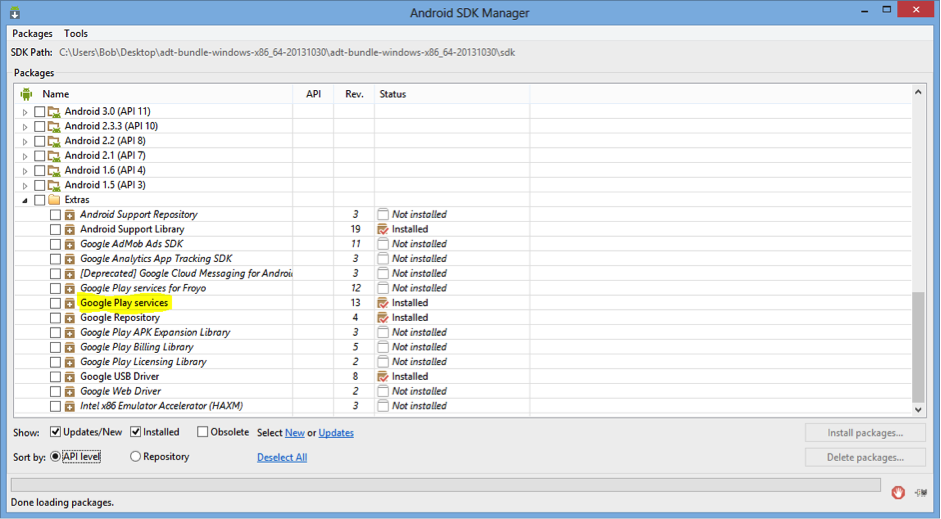
\includegraphics[width=\textwidth]{images/eclipse_sdk-manager}
\caption{SDK manager window of Eclipse showing Google Play Services}
\label{fig:eclipse-sdk-manager}
\end{figure}

\paragraph{} Requirements:

\begin{itemize}
\item Android device
\item Google Account (to get an API key)
\item Google Play Services Package
\end{itemize}

\subsection{Acquiring an API key}
\paragraph{} In order to use Google’s APIs you need an API key.  To get a maps key go to the Google APIs page\footnote{\url{https://code.google.com/apis/console}} and agree to the terms and conditions. You should now be on a page that looks similar to the following, browse down the list of APIs until you find “Google Maps Android API v2” and switch it to ON.

\begin{figure}[H]%[htb]
\centering
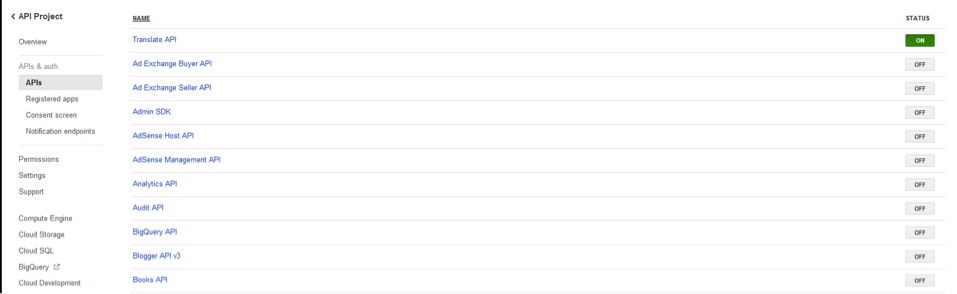
\includegraphics[width=\textwidth]{images/google-maps-api-page}
\caption{Google Maps API page}
\label{fig:google-maps-api-page}
\end{figure}

\paragraph{} Now that it’s on, go to ``Credentials'' on the left side and click the ``CREATE NEW KEY'' button and choose ``Android key''.  In the following text field you will need to provide the package name and SHA1 fingerprint. For package name type in zzcom.example.gmapsexample'' (NOTE: If you named your application something else use that name instead). To get your SHA1 fingerprint go to Window $>$ Preferences $>$ Android $>$ Build in Eclipse and copy the hexadecimal numbers from the SHA1 fingerprint box into the registration page. Once you click register, choose the “Android Key” option and copy the API key for use later.

\subsection{Preparing the Manifest}
\paragraph{} First things first, we need to import the Google Play Services to the workspace, go to File > Import > Existing Android Code Into Workspace.  Now browse to your SDK folder and go to 

\begin{framed}
Extras/google/google\_play\_services
\end{framed}
\paragraph{} Select the ‘libproject’ folder and click ok.

\begin{figure}[H]%[htb]
\centering
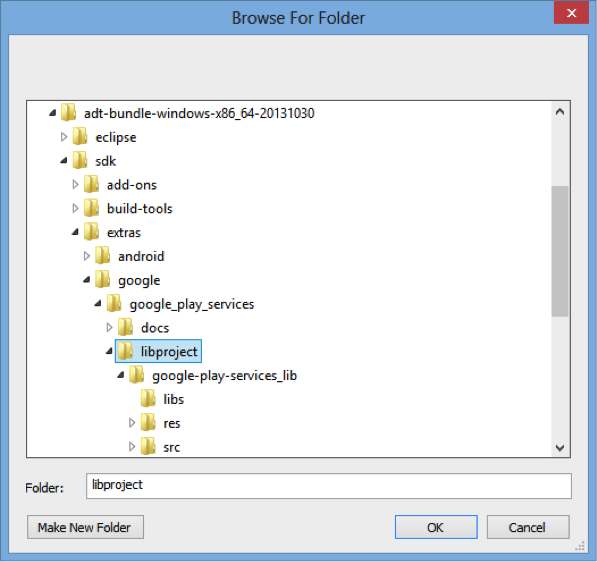
\includegraphics[width=0.75\textwidth]{images/libproject}
\caption{Google Maps API page}
\label{fig:libproject}
\end{figure}

\paragraph{} One project should be listed, check the “Copy projects into workspace” box then click finish. Now new Android Application named ‘GMapsExample’.  Now we need to add Google Play Services as a reference to our application. To do this, right click on your App in the package explorer and go to properties.  From properties go to Android on the left hand side and choose ‘Add…’ in the library section, highlight the “google-play-services\_lib” project and click ok.

\begin{figure}[H]%[htb]
\centering
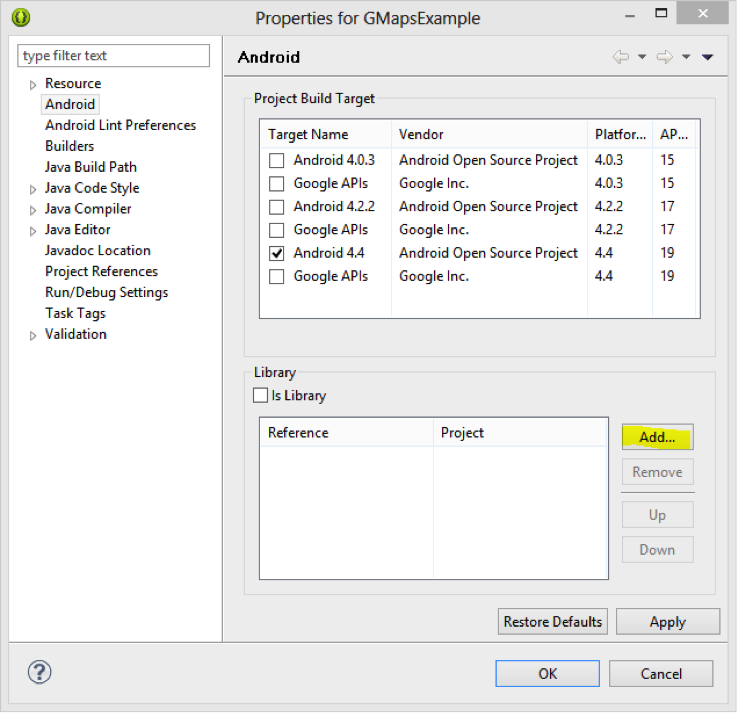
\includegraphics[width=0.75\textwidth]{images/gplay-services-lib}
\caption{Google Play Services Lib}
\label{fig:gplay-services-lib}
\end{figure}

\paragraph{} The final step to referencing play services is to add the following XML to our manifest within the <application> element.

\begin{lstlisting}
<meta-data
    	android:name="com.google.android.gms.version"
    	android:value="@integer/google_play_services_version" />
\end{lstlisting}

\paragraph{} Now that we have referenced the play services, we need to add the following permissions to our manifest to allow the application to get the users location and access Google’s servers.

\begin{lstlisting}
<!-- Used to download tiles from servers -->
<uses-permission android:name="android.permission.INTERNET" />
<!-- Used to check the network state to determine if data can be downloaded -->
<uses-permission android:name="android.permission.ACCESS_NETWORK_STATE" />
<!-- Used to cache map tiles -->
<uses-permission android:name="android.permission.WRITE_EXTERNAL_STORAGE" />
<!-- Allows access to google web services -->
<uses-permission android:name="com.google.android.providers.gsf.permission.READ_GSERVICES"/>
<!-- Allows app to access phones GPS information -->
<uses-permission android:name="android.permission.ACCESS_FINE_LOCATION" />
\end{lstlisting}

\paragraph{} Google Maps uses OpenGL ES v2 to render the map, we need to specify in the apps manifest that our app will be using this feature by adding the following to the manifest (just after the permissions).

\begin{lstlisting}
<uses-feature
        android:glEsVersion="0x00020000"
        android:required="true"/>
\end{lstlisting}

\paragraph{} Lastly we need to add the API key from the last step into our manifest. To do this simply copy the following section and paste it just after the other meta-data tags we added in the <application> element, remembering to replace the android:value value with your own API key.

\begin{lstlisting}
<meta-data android:name="com.google.android.maps.v2.API_KEY"
    		android:value="YOUR KEY HERE"/>
\end{lstlisting}

\subsection{Building the Application}
\paragraph{} Now that's all out the way we can get to building the app, the first step is to add a map fragment to your layout.  Open up your main\_activity layout and replace the XML with the following.

\begin{lstlisting}
<?xml version="1.0" encoding="utf-8"?>
<fragment xmlns:android="http://schemas.android.com/apk/res/android"
          android:id="@+id/map"
          android:layout_width="match_parent"
          android:layout_height="match_parent"
          android:name="com.google.android.gms.maps.MapFragment"/>
\end{lstlisting}

\paragraph{} If you run your app now you should get a screen looking something like this, if not then check your LogCat messages for any indication of what the issue may be. Often it will be an issue with API keys. Ensure the details of your application have been correctly registered on the API console and that you have correctly added your API key to the manifest and try again.

\begin{figure}[H]%[htb]
\centering
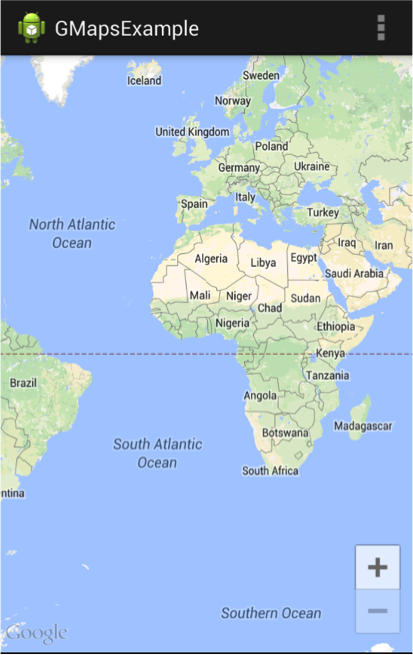
\includegraphics[width=0.5\textwidth]{images/google-map-example}
\caption{Google Map Screen}
\label{fig:google-map-example}
\end{figure}

\paragraph{} Now we’re going to make the map centre on the phones GPS position.  First set up a LocationManager and Listener just like section 4 of Week 3s tutorial, but this time replace the code inside the onLocationChanged function to the following.

\begin{lstlisting}
if (location != null) {
	GoogleMap map = ((MapFragment) getFragmentManager().findFragmentById(R.id.map)).getMap();
					
					map.moveCamera(CameraUpdateFactory.newLatLngZoom(new LatLng(location.getLatitude(), location.getLongitude()), 13));
}
\end{lstlisting}

\paragraph{} The first line here retrieves the map fragment from the layout and stores it in a variable called map (much like findViewById does for buttons and such) while the second line moves the camera by using a CameraUpdateFactory and providing it with a new LatLng object (created using the latitude and longitude values from the location variable) and a zoom level.

\paragraph{Extra Tasks} Try adding some buttons to the application that take you directly to different places.

\subsection{More Features}

\paragraph{} There are several other ways we can interact and modify the maps.  We can choose between the following:

\begin{itemize}
\item Normal – Roads, man-made features and important natural features (eg rivers) shown
\item Hybrid – Satellite picture with roads added
\item Satellite – Satellite picture, no roads added
\item Terrain – Topographic data, includes colours/contour lines
\end{itemize}

\paragraph{} To choose a different map style we simple have to call the setMapType function and tell it which type we want.

\begin{lstlisting}
map.setMapType(GoogleMap.MAP_TYPE_SATELLITE);
/* GoogleMap.MAP_TYPE_NORMAL
 * GoogleMap.MAP_TYPE_HYBRID
 * GoogleMap.MAP_TYPE_TERRAIN
 */
\end{lstlisting}

\paragraph{} The following shows an example of normal, hybrid and terrain maps for the same location.

\begin{figure}[H]%[htb]
\centering
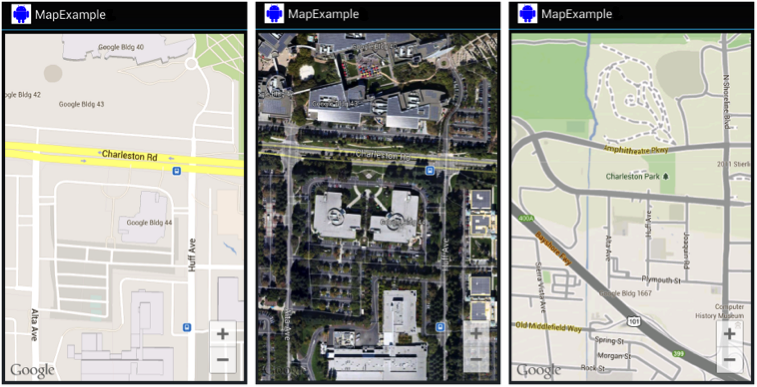
\includegraphics[width=\textwidth]{images/normal-hybrid-terrain-map-examples}
\caption{Examples of Normal, Hyrbid, \& Terrain Google Maps}
\label{fig:normal-hybrid-terrain-map-examples}
\end{figure}

\subsubsection{Markers}
\paragraph{} We can also draw several different things onto the maps such as markers or information windows.  Adding a marker onto Edinburgh Castle is as simple as the following.

\begin{lstlisting}
LatLng edCastle = new LatLng(55.948611, -3.200833);
map.addMarker(new MarkerOptions().position(edCastle));
\end{lstlisting}

\paragraph{} The first line creates a LatLng object with the coordinates of Edinburgh Castle and the second line adds a new marker to the map object at the coordinates of edCastle.  You can add loads of other options to your markers such as making them draggable, changing their colour, using your own image as the marker icon or even adding click or drag events to the markers.  For more information on how to customise your markers see the Marker documentation\footnote{\url{https://developers.google.com/maps/documentation/android/marker\#customize_a_marker}}.

\subsubsection{Information Windows}
\paragraph{} Markers are great for, well, marking a position on the map.  However sometimes we want to display some information at a point on the map.  To do this we can use info windows.  To do this we create a marker on the map much the same as we did before, except this time we give it a title and snippet.  Replace your marker from the last step with the following

\begin{lstlisting}
map.addMarker(new MarkerOptions().position(edCastle).title("Edinburgh Castle").snippet("Historic fortress which dominates the skyline of the city of Edinburgh, Scotland"));
\end{lstlisting}

\paragraph{} Run the application again, you’ll see a marker on Edinburgh Castle much like before except this time when you click it some extra information will be shown

\begin{figure}[H]%[htb]
\centering
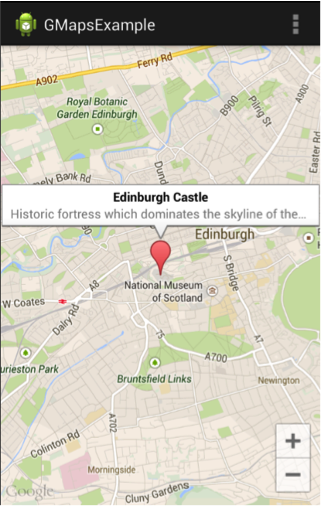
\includegraphics[width=0.5\textwidth]{images/google-map-info-marker}
\caption{Google Map Marker Example}
\label{fig:google-map-info-marker}
\end{figure}


\section{Summary}
\paragraph{} In this practical we have 

\begin{itemize}
\item Retrieve data from Web Service APIs using JSON
\item Use Google Services
\end{itemize}



\chapter{Sensing}
\section{Aims}
\paragraph{} At the end of the practical portion of this topic you will be able to:

\begin{itemize}
\item Use GPS \& the Android location API to find \& work with your location
\item Use the Android sensor API
\end{itemize}

\section{GPS}
\paragraph{} To access the GPS hardware we need to add a permission to our Android Manifest. Create a new Android project and delete the `Hello World' TextView. Open the AndroidManifest.xml file and add the following line:

\begin{lstlisting}
<uses-permission android:name="android.permission.ACCESS_FINE_LOCATION"/>
\end{lstlisting}

\paragraph{} between the $<$manifest ....$>$ $<$/manifest$>$ tags, e.g.

\begin{lstlisting}
<?xml version="1.0" encoding="utf-8"?>
<manifest xmlns:android="http://schemas.android.com/apk/res/android"
    package="org.simonwells.testgps" >

    <uses-permission android:name="android.permission.ACCESS_FINE_LOCATION"/>

    <application
        android:allowBackup="true"
        android:icon="@drawable/ic_launcher"
        android:label="@string/app_name"
        android:theme="@style/AppTheme" >
        <activity
            android:name=".MainActivity"
            android:label="@string/app_name" >
            <intent-filter>
                <action android:name="android.intent.action.MAIN" />

                <category android:name="android.intent.category.LAUNCHER" />
            </intent-filter>
        </activity>
    </application>

</manifest>
\end{lstlisting}

\paragraph{} To actually use this we need two things. First, some Java code in our app to retrieve and do something with the GPS data, and secondly, to supply some GPS data to our app. Let's start with the code then mess with the data later. All we are going to do is create a LocationListener that controls doing something with GPS data when we recieve it, and a LocationManager to call the LocationListener when there is GPS data. Both LocationListener and LocationManager are part of the Android libraries so we will need to import those (along with some supplementary classes like Toasts and Contexts to help us). These are changes to our java code so we need to edit MainActivity.java and afterwards it should look something like this:

\begin{lstlisting}
package org.simonwells.testgps;

import android.content.Context;
import android.location.Location;
import android.location.LocationListener;
import android.location.LocationManager;
import android.support.v7.app.ActionBarActivity;
import android.os.Bundle;
import android.view.Menu;
import android.view.MenuItem;
import android.widget.Toast;


public class MainActivity extends ActionBarActivity {

    LocationManager locationManager = null;
    LocationListener locationListener = null;

    @Override
    protected void onCreate(Bundle savedInstanceState) {
        super.onCreate(savedInstanceState);
        setContentView(R.layout.activity_main);

        locationManager = (LocationManager)getSystemService(Context.LOCATION_SERVICE);

        locationListener = new LocationListener() {
            @Override
            public void onLocationChanged(Location location) {
                if (location != null) {
                    String locationStr = "Location changed. Lat: " +
                            location.getLatitude() + " lon: " + location.getLongitude();

                    Toast.makeText(getBaseContext(), locationStr, Toast.LENGTH_SHORT).show();
                }
            }

            @Override
            public void onStatusChanged(String provider, int status, Bundle extras) {

            }

            @Override
            public void onProviderEnabled(String provider) {

            }

            @Override
            public void onProviderDisabled(String provider) {

            }
        };

        locationManager.requestLocationUpdates(LocationManager.GPS_PROVIDER, 0, 0, locationListener);
    }

    @Override
    protected void onPause() {
        super.onPause();
        locationManager.removeUpdates(locationListener);
        String status = locationManager.toString();
        Toast.makeText(getApplicationContext(), status, Toast.LENGTH_SHORT).show();
    }


    @Override
    public boolean onCreateOptionsMenu(Menu menu) {
        // Inflate the menu; this adds items to the action bar if it is present.
        getMenuInflater().inflate(R.menu.menu_main, menu);
        return true;
    }

    @Override
    public boolean onOptionsItemSelected(MenuItem item) {
        // Handle action bar item clicks here. The action bar will
        // automatically handle clicks on the Home/Up button, so long
        // as you specify a parent activity in AndroidManifest.xml.
        int id = item.getItemId();

        //noinspection SimplifiableIfStatement
        if (id == R.id.action_settings) {
            return true;
        }

        return super.onOptionsItemSelected(item);
    }
}
\end{lstlisting}

\paragraph{} Notice in this case that we have declared the variables to store our location Manager and location listener in our MainActivity class. This is so that we can reference those variables in places besides the onCreate method. For example, we want our app to stop listening for GPS data when our activity loses visibility so we have implement an onPause method which removes our location listener from the location manager. You should consider the other methods that make up the activity lifecycle if you want to resume GPS tracing when the app is made visible again.

\paragraph{} Supplying data is straightforward if you are using a hardware device, just turn on GPS and ensure that you are somewhere where you can receive GPS signals (e.g. outside). If you are using the AVD to emulate a hardware device then you need to use the AVD controls from within your IDE (either within Android Studio or Eclipse) to inject fake GPS data into the running AVD. To do this we need to introduce ourselves to another tool from the Android SDK, the Dalvik Debug Monitor Service (DDMS) which is available in Eclipse by going to Window $>$ Open Perspective $>$ DDMS. To exit the DDMS to edit code again then you can go to Window $>$ Close Perspective. In the DDMS selectthe Emulator tab and you should see a `Location Controls' section in which you can set a Latitude or Longitude value and a `send' button to send the coordinates to the AVD.

\paragraph{} You can use Google Maps to retrieve the coordinates of a given location by right-clicking on the map and selecting `what's here?'. The coordinates will then be displayed in a box along with the street address. You can copy these coordinates and supply them to your AVD via the DDMS if you want to test specific locations for your app.

%\section{Location API}
%\paragraph{}

\section{Sensors}
\paragraph{} The Android platform supports many sensors. These include motion, enivronmental, and position sensors. In this practical we shall use the accelerometer, but the basic principles for using sensors in your app are the same. Also it is important to notice that whilst you can write an app that uses sensors you must either use hardware that includes your target sensor to test it, or else use a third party tool such as the Open Intents Sensor Simulator\footnote{\url{https://code.google.com/p/openintents/wiki/SensorSimulator}} to supply simulated sensor data to the Android AVD.

\paragraph{} Let's get started. We are going to write some Java code that uses the android.hardware.Sensor libraries to check what sensors are available then to retrieve a handle for the accelerometer. We are then going to use a SensorEventListener to do something with the accelerometer data each time the listener hears an update.

\paragraph{} Create a new Android project and delete the `Hello World' TextView. We are not going to use any other views or layout elements in this pracical, just Toasts to output our data in the easiest way possible. You can however use this practical as a building block to integrate sensor data with a more advanced UI.

\paragraph{} Your MainActivity.java should end up looking something like this (it's a lot of code but we shall go through it over the next few paragraphs):

\begin{lstlisting}
package org.simonwells.testsensors;

import android.content.Context;
import android.hardware.Sensor;
import android.hardware.SensorEvent;
import android.hardware.SensorEventListener;
import android.hardware.SensorManager;
import android.support.v7.app.ActionBarActivity;
import android.os.Bundle;
import android.view.Menu;
import android.view.MenuItem;
import android.widget.Toast;

public class MainActivity extends ActionBarActivity {

    private long lastUpdate = 0;
    private float last_x, last_y, last_z = 0;
    private static final int SHAKE_THRESHOLD = 600;

    @Override
    protected void onCreate(Bundle savedInstanceState) {
        super.onCreate(savedInstanceState);
        setContentView(R.layout.activity_main);
        SensorManager mSensorManager = (SensorManager) getSystemService(Context.SENSOR_SERVICE);
        Sensor sensorAccel;

        if (mSensorManager.getDefaultSensor(Sensor.TYPE_ACCELEROMETER) != null) {
            Toast.makeText(getBaseContext(), "HAS ACCELEROMETER", Toast.LENGTH_LONG).show();

            sensorAccel = mSensorManager.getDefaultSensor(Sensor.TYPE_ACCELEROMETER);
            mSensorManager.registerListener(new SensorEventListener() {
                @Override
                public void onSensorChanged(SensorEvent event) {
                    Sensor localSensor = event.sensor;

                    if (localSensor.getType() == Sensor.TYPE_ACCELEROMETER){
                        float x = event.values[0];
                        float y = event.values[1];
                        float z = event.values[2];

                        long curTime = System.currentTimeMillis();

                        if ((curTime - lastUpdate) > 100)
                        {
                            long diffTime = (curTime - lastUpdate);
                            lastUpdate = curTime;

                            float speed = Math.abs(x + y + z - last_x - last_y - last_z)/ diffTime * 10000;

                            if (speed > SHAKE_THRESHOLD)
                            {
                                String str = String.valueOf(x) + String.valueOf(y) + String.valueOf(z);
                                Toast.makeText(getBaseContext(), str, Toast.LENGTH_SHORT).show();
                            }
                            last_x = x;
                            last_y = y;
                            last_z = z;
                        }
                    }
                }

                @Override
                public void onAccuracyChanged(Sensor sensor, int accuracy) {

                }
            }, sensorAccel, SensorManager.SENSOR_DELAY_NORMAL);

        }
        else
            Toast.makeText(getBaseContext(), "NOPE",Toast.LENGTH_LONG).show();
    }

    @Override
    public boolean onCreateOptionsMenu(Menu menu) {
        // Inflate the menu; this adds items to the action bar if it is present.
        getMenuInflater().inflate(R.menu.menu_main, menu);
        return true;
    }

    @Override
    public boolean onOptionsItemSelected(MenuItem item) {
        // Handle action bar item clicks here. The action bar will
        // automatically handle clicks on the Home/Up button, so long
        // as you specify a parent activity in AndroidManifest.xml.
        int id = item.getItemId();

        //noinspection SimplifiableIfStatement
        if (id == R.id.action_settings) {
            return true;
        }

        return super.onOptionsItemSelected(item);
    }
}
\end{lstlisting}

\paragraph{} In the MainActivity class we have created some private variables, e.g. lastUpdate, last\_x, last\_y, last\_z, and SHAKE\_THRESHOLD, that we will use later in the various methods and listeners that we implement. All our other edis are in the OnCreate method where we have created a SensorManager\footnote{\url{http://developer.android.com/reference/android/hardware/SensorManager.html}} and a Sensor\footnote{\url{http://developer.android.com/reference/android/hardware/Sensor.html}} object. There are a lot of sensor types available, including the accelerometer (TYPE\_ACCELEROMETER), thermometer (TYPE\_AMBIENT\_TEMPERATURE), gyroscope (TYPE\_GYROSCOPE), magnetometer (TYPE\_MAGNETIC\_FIELD), and many others. Check out the Android sensor documentation linked in the footnotes for details of the full list of types that are currently supported. Obviously you can only actually use those sensors that your hardware includes when running your app.
\paragraph{} The SensorManager is used to get access to the sensors supported by the hardware on which our app is running, and access to these is provided by the Android system. We first use the SensorManager to check whether an accelerometer exists then, if it does, we use the SensorManager to get a reference to the accelerometer sensor so that we can use it. Notice that we have used a Toast to give quick output to say whether the accelerometer is available or not. Once we have a reference to the accelerometer sensor we then create and register a new SensorEventListener for it. We have then overriden the base methods for onSensorChanged and onAccuracyChanged, both of which we are required to deal with to use this kind of listener. However, we are only going to deal with detected sensor changes so we only add some code to the onSensorChanged method for now. The important part to notice of onSensorChanged is the assignements of x, y, and z values from the supplied event into local float variables. The accelerometer works in three dimensions so we get a value supplied to us for each dimension. The code for the rest of this method is purely to do something with the supplied x, y, and z values. Basically, make sure that the last update was at least 100 milliseconds agothen determine how much the sensor has moved, our {\emph{speed}}, sinse the last detection. If the  speed is greated than our threshold then we assemble a string and display it using a Toast.

\section{Summary}
\paragraph{} In this practical we have 

\begin{itemize}
\item Used GPS \& the Android location API to find \& work with our location
\item Used the Android sensor API to work with the accelerometer sensor
\end{itemize}




\part{Notes}

\chapter{Introduction to Mobile Computing} 

\section{Aims}
\paragraph{} At the end of this topic you will be able to:

\begin{itemize}
\item Explain where ‘mobile app’ development fits into the recent history of computing \& mobile computing. 
%\item Develop an Android app % In 2016 will include Hello Android but not in 2015
\end{itemize}


\section{The Rise of Mobile Computing}
\paragraph{} Today's mobile phone owes its origins to radio phones which were introduced on first class passenger trains in Germany in 1926. Mobile technology was enhanced during WW2 when Motorola created a walkie-talkie for the US Army – which was carried in a backpack to house the huge batteries.

\paragraph{} Following the development of cell-based transmitters and receivers in the late 1940s, the 1950s saw car phones making use of this cell technology although calls were not continuous as the car travelled from one cell to the next.

\paragraph{} In 1956 Ericsson created the first system that did not require manual control in the base stations in Sweden. Unfortunately the phone weighed 40 kilograms so not mobile in the sense we understand today.

\paragraph{} Until 1970 mobile technologies continued to be developed mainly in US and USSR. In 1971 an engineer from Bell Labs found a solution for transferring the call from a network to another without loss of communication. In 1973 Motorola made its first call on a truly mobile phone, illustrated in Figure \ref{fig:brick-phone}, – which is now referred to as the first generation. After specialising in military communications, Vodaphone launched the UKs mobile network in 1985. By the mid to late 1980s the mobile phone was the must have status symbol of business wheelers and dealers in Thatcherite Britain.

\begin{figure}[htb]
\centering
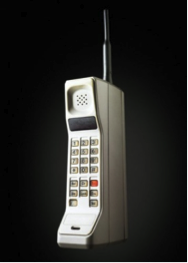
\includegraphics[width=0.5\textwidth]{images/brick-phone}
\caption{Motorola's mass marketed phone from 1973}
\label{fig:brick-phone}
\end{figure}

\paragraph{} In the 1990s the second generation of phones appeared – introducing digital technology in the form of GSM (Global System for Mobile communications) into the networks. In Europe Nokia was a key developer of GSM and the first GSM network was opened in Finland. This second generation of mobile phones introduced the SMS service – arguably the start of social networking. Customisation started here – with downloadable, if expensive, ring tones – and business users were overtaken by the general population driven by a huge interest from younger users.

\paragraph{} Third generation networks \& devices appeared in Japan in 2001. The main aim was to satisfy the demand for data services  i.e. move to packet switching to speed things up so we could get internet-on-the-go, swap photos and video. The i) mobile phone and ii)PDAs/ netbooks with dongles started to converge with the smartphone emerging as the product of their convergence. 

\paragraph{} The fourth generation is fast approaching – VoIP will replace traditional circuit switched calls in a network optimised for data services. At the moment it’s just a marketing term.

\section{Recent History of Mobile Computing}

\begin{itemize}

\item The first commercial laptop illustrated in Figure \ref{fig:grid-compass}, the GRiD Compass\footnote{\url{http://en.wikipedia.org/wiki/Grid_Compass}} started selling in 1982 at a price tag of \$8000 the main customer was the US Department of Defence and NASA.

\item Personal Digital Assistant was a term used to describe the Apple Newton  illustrated in Figure \ref{fig:apple-newton}, first sold in 1992. PDAs could keep calendars, play games, synch with your desktop. Although there was a proliferation of manufacturers' operating systems, the Symbian OS came to dominate, with MS following with their Microsoft CE OS.

\item The Nokia 9000  illustrated in Figure \ref{fig:nokia-9000}, was released 1996. A phone which could send/receive emails and type up Word docs. Arguably the world's first smartphone.

\item In 2002, Blackberry manufacturers Re-search in Motion (RIM) released their first smartphone,  illustrated in Figure \ref{fig:rim-blackberry}, following their successful push email technology. Popular amongst business users originally, the Blackberry found a new market amongst teenage girls thanks to the BlackBerry Messenger app, before declining in popularity.

\item The first Apple iPhone, illustrated in Figure \ref{fig:apple-iPhone}, was released in June 2007. The latest version, 4, was released in July 2010 (following the iPad release in April 2010). The iPhone was the first smartphone with mass market appeal.

\item In October 2008, the first Android phone – the HTC Dream (aka T-Mobile G1), illustrated in Figure \ref{fig:android-phone}, – was released. This was followed by the HTC Hero and now HTC Desire \& Samsung Galaxy, among others. Encouraged by the open nature of the development kit, this is creating a garage app developer culture.

\end{itemize}

\begin{figure}[htb]
        \centering
        \begin{subfigure}[b]{0.3\textwidth}
                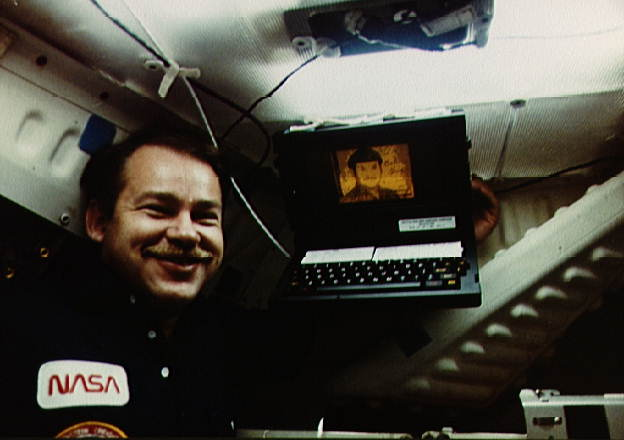
\includegraphics[width=\textwidth]{images/grid-compass}
                \caption{GRiD Compass}
                \label{fig:grid-compass}
        \end{subfigure}%
        ~ %add desired spacing between images, e. g. ~, \quad, \qquad, \hfill etc.
          %(or a blank line to force the subfigure onto a new line)
        \begin{subfigure}[b]{0.3\textwidth}
                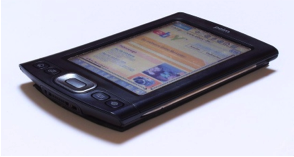
\includegraphics[width=\textwidth]{images/apple-newton}
                \caption{Apple Newton}
                \label{fig:apple-newton}
        \end{subfigure}
        ~ %add desired spacing between images, e. g. ~, \quad, \qquad, \hfill etc.
          %(or a blank line to force the subfigure onto a new line)
        \begin{subfigure}[b]{0.3\textwidth}
                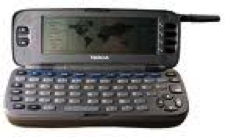
\includegraphics[width=\textwidth]{images/nokia-9000}
                \caption{Nokia 9000}
                \label{fig:nokia-9000}
        \end{subfigure}
        \caption{The GRiD Compass, Apple Newton, \& Nokia 9000}\label{fig:early-mobile-platforms-1}
\end{figure}

\begin{figure}[htb]
        \centering
        \begin{subfigure}[b]{0.3\textwidth}
                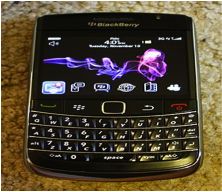
\includegraphics[width=\textwidth]{images/rim-blackberry}
                \caption{RIM Blackberry}
                \label{fig:rim-blackberry}
        \end{subfigure}%
        ~ %add desired spacing between images, e. g. ~, \quad, \qquad, \hfill etc.
          %(or a blank line to force the subfigure onto a new line)
        \begin{subfigure}[b]{0.3\textwidth}
                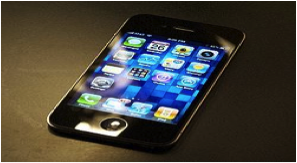
\includegraphics[width=\textwidth]{images/apple-iphone}
                \caption{Apple iPhone}
                \label{fig:apple-iPhone}
        \end{subfigure}
        ~ %add desired spacing between images, e. g. ~, \quad, \qquad, \hfill etc.
          %(or a blank line to force the subfigure onto a new line)
        \begin{subfigure}[b]{0.3\textwidth}
                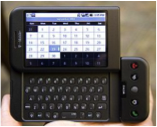
\includegraphics[width=\textwidth]{images/android-phone}
                \caption{Android Phone}
                \label{fig:android-phone}
        \end{subfigure}
        \caption{The Blackberry, iPhone, \& Android}\label{fig:early-mobile-platforms-1}
\end{figure}



\paragraph{} \emph{Where are we now?} The line between communication and computation has become increasingly blurred. A smartphone is now a handheld computer with integrated mobile phone (and pager, compass, camera, GPS, torch, ...)

\begin{quote}
"I have always wished for my computer to be as easy to use as my telephone; my wish has come true because I can no longer figure out how to use my telephone." 
— Bjarne Stroustrup  (Danish inventor of C++)
\end{quote}

\paragraph{} What do we expect of our mobile computing devices?
\begin{itemize}
\item phone
\item touchscreen or at least easy character entry
\item email
\item camera \& memory to save photos
\item audio \& video recorder \& player
\item web browsing
\item app platform eg games
\item reasonable battery life
\item small?
\end{itemize}

\paragraph{} Less discerning about:
\begin{itemize}
\item price - not necessarily cost conscious, at the moment
\item shelf life
\end{itemize}

\paragraph{} So what's the current state of play? Check with Gartner, market analysts. Android phones and iPhones continue to increase their market share.  New markets include the developing world – Huawei Telecom in China are manufacturing cheap Androids for India and Africa. There is also growth in iPad/ Android tablets.
 

 %%
 %%
 %% INSERT SECTION ON GARTNER SALES FIGURES
 %%
 %%
 %%


 \paragraph{} To a large extent the availability of apps is driving these increases for the iPhone and Android. Blackberry launched their own apps market and saw some growth in their handset sales. Meanwhile Symbian have opened up their OS. Huawai Telecom have launched a cheap Android phone in India – the Ideo. It’s hard to see a way for the iPhone to reach the developing world.


\section{Summary}
\paragraph{} In this topic we have attempted to understand why mobile computing and communication have become popular now by studying longer term trends in the wider fields of computing and communication.

\section{Directed Study}
\paragraph{} 

\begin{itemize}
\item Read Chapters 1 to 3 of Android Wireless Application Development \cite{conder_2010_android_ebook}.
\item Read more about the history of mobile computing, for example the Wikipedia page on the history of mobile phones is a good place to start\footnote{\url{http://en.wikipedia.org/wiki/History_of_mobile_phones}}.
\item Visit the developers website http://developer.android.com
\item Check your understanding of the topic by answering the following:
\begin{enumerate}
\item Name three apps you have used/ heard about and identify the platform they run on?
\item What makes a good app?
\item In Android-speak, what is an activity?
\item How do Intents work?
\end{enumerate}
\item If you have access to a computer at home, download and install the Oracle Java JDK\footnote{\url{http://www.oracle.com/technetwork/java/javase/downloads/index.html}} then install the Android development tools\footnote{\url{http://developer.android.com/sdk/index.html}}.
\item Have a look at the App Inventor\footnote{\url{http://appinventor.mit.edu/}}  – what do you think – can this revolutionise app development? It was initially developed by Google then, when abandoned, MIT stepped in.
\end{itemize}


%\section{Resources}


\chapter{Platforms \& Lifecycles}

\section{Aims}
\paragraph{} At the end of this topic you will be able to:

\begin{itemize}
\item Describe what Android is
\item Describe and use the Android SDK
\item Select and use an IDE
\item Understand the components of an Android App
\item Understand the Activity life-cycle
\end{itemize}

\section{Introducing Android} 
\paragraph{} As you can see we have lots of options for how to develop software for mobile devices. For the practical part of this module, we are going to use Android.

\begin{framed}
\begin{quote}
Android is Google's operating system for mobile devices based on ARM architecture. It is a competitor to the Symbian platform, Apple's iOS for the iPhone and Microsoft's Windows Mobile and Windows Phone for mobile devices all based on ARM architecture.
Android sits on a modified Linux kernel and includes middleware which allow you access to the hardware and key applications. It lets you develop Java but, as with applets on the web, there are some constraints and a philosophical framework.
The Android operating system software stack consists of Java applications running on a Java based object oriented application framework on top of Java core libraries running on a Dalvik virtual machine featuring JIT compilation. … The Android operating system consists of 12 million lines of code including 3 million lines ofXML, 2.8 million lines of C, and 2.1 million lines of Java
\end{quote}

{\begin{flushright}Source: Wikipedia\\\url{http://en.wikipedia.org/wiki/Android_(operating_system)}\end{flushright}}
\end{framed}

\paragraph{} Android was launched by Google/Open Handset Alliance in November 2007 with a competition for developers to design and build prize winning apps – they offered \$1m in prize money. This kick started the Android marketplace. One of the winning apps was an automatic taxi ordering service which read your location in New York and with a single button press ordered a taxi to pick you up; perhaps reason enough to buy a phone?\footnote{See more winners at \url{http://code.google.com/android/adc/gallery_winners.html}}


\section{Development Tools}
\subsection{The SDK}
\paragraph{} The Android SDK is the core set of tools that the Android project have released so that we can develop our own Android apps. The SDK is a mix of tools, that work primarily from the command line, and libraries, which your code can hook into to make use of Android platform features. Whilst the tools work from the command line, there is additional software that you can use to provide graphical user interfaces to the Android tools. For example, Android Studio is an Integrated Development Environments (IDE) which provide a graphical development environment to the command line tools of the SDK. You can build Android apps using only the SDK, however many developers feel more comfortable using an IDE.

\subsection{Development Environments}
\paragraph{} Since December 2014 when version 1.0 was released, the main IDE for Android development has been Android Studio. Prior to this the main IDE was Eclipse, a popular Java development IDE with additional plugins to support Android development. 

\subsection{The Android Debug Bridge}
\paragraph{} Because Android apps are designed and built to run on devices using the Android OS, and not your desktop OS such as Linux, Mac OS, or Windows, you need to provide a way for any apps that you produce to run so that you can test them. For this you have a few options, but you must do at least one of these if you want to be able to run your Android app (and determine that it runs correctly):

\begin{enumerate}
\item The Android Emulator/Android Virtual Device (AVD) - Your IDE provides tools that allow you to run a program that emulates an Android device. In Studio these can be found under Tools $>$ Android $>$ AVD Manager. AVD stands for Android Virtual Device which is the emulated version of the Android OS. Use the AVD Manager to create new devices with various hardware capabilities and software levels. However you should note that emulation is very very very slow. In particular on lab machines, which are running the emulation across the network, you must create AVDs which are very conservative in their hardware, e.g. use lower amounts of RAM, 256MB should be sufficient for most lab practicals, and which use a smaller screensize, e.g. 
\item Hardware - If you have an Android device then you can enable the USB Debugging mode, plug it into your development machine, and it should appear as a connected device which you can select as a target to run your app on. This mode is hidden in a different place on different Android devices so you might have to do a web search for your ``device name+model+enable USB debugging mode''. On OS X and Linux this should 'just work'. On Windows you may have to install drivers for your mobile device before it can be recognised and used to debug Android apps.
\item Virtual Machine - Genymotion\footnote{\url{https://www.genymotion.com/}} is probably the best third party solution for faster virtual Android devices. Underneath it uses the VirtualBox virtualisation software and is much faster than the AVD approach.
\end{enumerate}


\section{Architecture of the Android Platform}
 
\begin{figure}[htb]
\centering
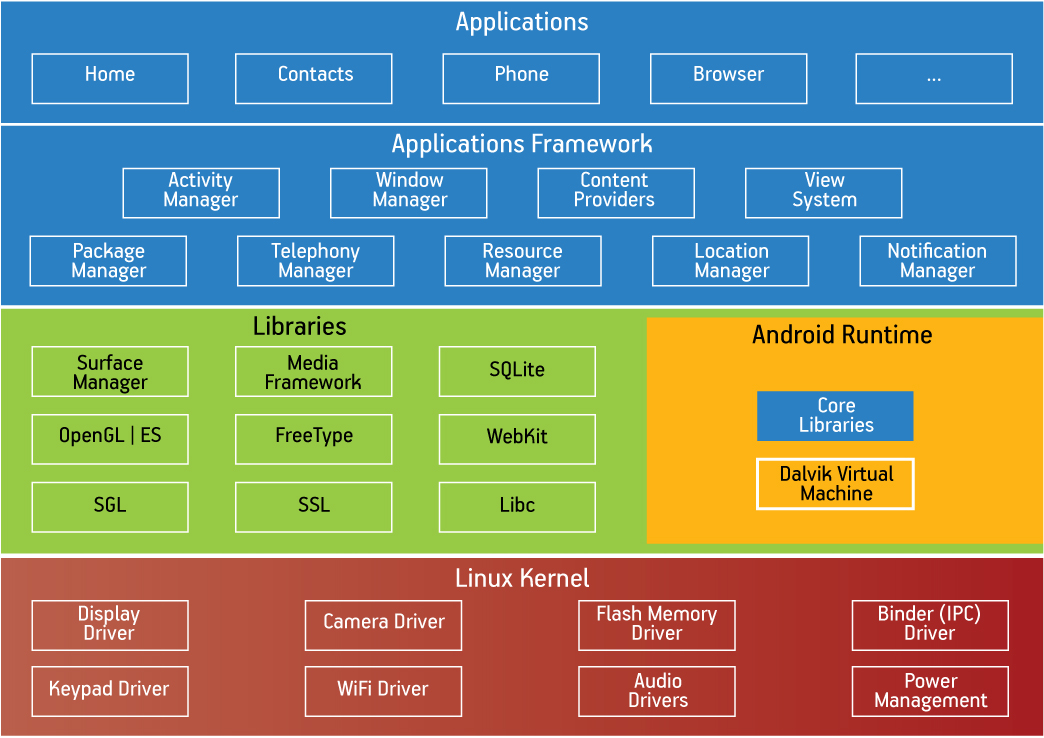
\includegraphics[width=\textwidth]{images/architecture-android}
\caption{The architecture of the Android platform}
\label{fig:architecture-android}
\end{figure}

\section{The Components of apps}
\paragraph{} Android has been designed to let developers take advantage of all the hardware nestling inside your phone. It does this through activities which “do stuff”, services which “do background stuff”,  reusing another app’s functionality (if granted permission) and publishing functionality. Specifically an application is made up of components and a messaging service to communicate between them:

\subsection{Activities}
Think of as a single view or window and one per screen – you can move pages by launching another activity. User interface components are called Views and include scroll-bars, text strings etc (similar to swing components in Java or controls in VS).

\subsection{Services}
A service doesn't have a visual user interface. They run in the background. For example, a service might play background music. Each service extends the Service base class.

\subsection{Broadcast Receivers}
A broadcast receiver is a component that responds to system-wide announcements, for example, that the music player has been switched on, that the battery is low. Your app can also broadcast some information for other apps running on the phone – and interested apps can, as BroadcastReceivers, receive the message (eg change of timezone) and apps can also be BroacastReceivers by extending the BroadcastReceiver base class. You might want to notify the user - through the NotificationManager. These notifications appear on the status bar.

\subsection{Content Provider}
A wrapper for databases and files, the content provider can make app data available to other apps

\section{The Activity Lifecycle}


\begin{figure}[htb]
\centering
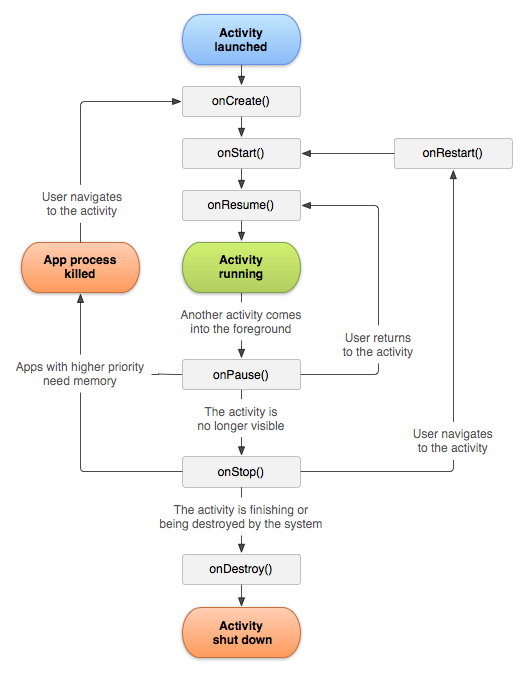
\includegraphics[width=0.8\textwidth]{images/android_lifecycle_original}
\caption{The lifecycle of Android activities.}
\label{fig:lifecycle-android-activities}
\end{figure}


\begin{figure}[htb]
\centering
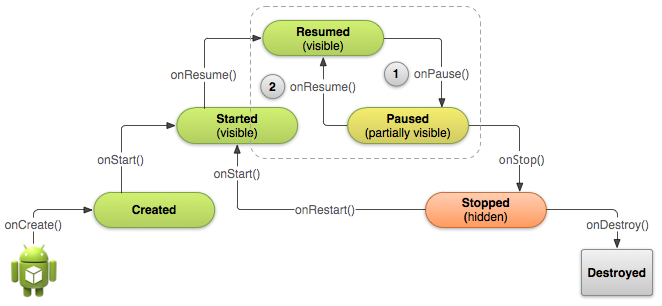
\includegraphics[width=\textwidth]{images/android_lifecycle_state-diagram}
\caption{A slightly re-arranged diagram of the lifecycle of Android activities.}
\label{fig:lifecycle-android-activities-state-diargram}
\end{figure}



\paragraph{} Activities and services are activated by intents. Intents are asynchronous messages used by the OS to match task requests with activities and services. The Intent object is a bundle of information: it ``contains information of interest to the component that receives the intent (such as the action to be taken and the data to act on) plus information of interest to the Android system (such as the category of component that should handle the intent and instructions on how to launch a target activity)''\footnote{\url{http://developer.android.com/guide/topics/intents/intents-filters.html}}.


\paragraph{} Instead of a main method defining where things kick off, you must define a class which extends (or inherits from) Activity. An Activity class simply means that it can run and do stuff.
The onCreate() method will be called when your Activity starts — it is where you should perform all initialization and UI setup. The onCreate() method will be called by the Android system when your Activity starts — it is where you should perform all initialization and UI setup. [The @Override statement is a Java convention - it simply flags up your intention to override a method in the superclass so the compiler can check that’s what you actually end up doing – and flag it if that’s not what the net effect is.] The Bundle is a mechanism for living with the complexity of multiple activities, multiple entry points etc. The bundle refers to the data required to run your activity effectively – eg what is the current state of your activity, have you been interrupted by a phone call for example.
A View is a drawable object eg button, image or, in this case, some text. TextView is a subclass of view. We construct a TextView object (tv). The constructor parameter this refers to is an Android Context. A Context is a handle to the system – providing preferences, access to databases etc. The Activity class inherits from the Context so this is a context.  
The app then calls the setText() method of the tv object.
Finally, you pass the tv to setContentView() in order to display it as the content for the Activity UI. If your Activity doesn't call this method, then no UI is present and the system will display a blank screen.




\section{Summary}
\paragraph{} In this topic we have learnt to:

\begin{itemize}
\item Describe what Android is
\item Describe and use the Android SDK
\item Select and use an IDE
\item Understand the components of an Android App
\item Understand the Activity life-cycle
\end{itemize}


%\section{Directed Study}
%\paragraph{}

%\section{References \& Resources}


\chapter{Mobile User Experience}

\section{Aims}
\paragraph{} At the end of this topic you will be able to:

\begin{itemize}
\item Use design patterns to communicate your designs
\item Use and understand platform guidelines
\item Evaluate your application
\end{itemize}

\paragraph{} Whilst there are many core lessons to be learnt from human factors research about the best ways to design software for different users which are generally applicable, it is also true that the mobile platform offers some aspects of the user experience which are particular to the mobile context. For example, the close integration of a wide array of physical sensors, human and machine oriented communication support, wide-variety of screen sizes, touch interface, lack of hardware keyboard, wireless/untethered operation, and pure ubiquitousness provide both unique opportunities to take advantage of and novel pitfalls to avoid.


\section{Design Patterns}
\paragraph{} Design patterns can be considered as an attempt to build a shared language for describing solutions to problems. They were originated in the architectural research discipline by Christopher Alexander who coined the term ``Pattern Language''. An individual pattern describes a problem, and a solution. Importantly, patterns were originally specified as `timeless' e.g. they didn't make assumptions about the adoption of a particular technology or intricate solution to a one-off issue, but were more about dealing with recurring problems that have accepted and acknowledged solutions that are both beautiful and practical. A key element of patterns is the idea of language. A collection of design patterns forms a shared language for communicating ideas about recognising and solving problems. By having a shared language people, any people, not just experts, can understand and contribute towards the solution of the problem.

\subsection{Patterns as a Dictionary of Decisions}
\paragraph{} One nice way to describe patterns is as entries in a dictionary. When a designer creates a design they make decisions about how to solve problems. Often these problems and solutions recur many times in many contexts. A pattern is thus a single, documented problem and its most common, recognised, good solution. Each pattern is named, described, and cross-referenced to related patterns similar to entries in a dictionary. In this way the collection of patterns form a language, having syntax, the description of individual patterns, grammar and semantics, captured by the relations between patterns.

\paragraph{} The idea of pattern languages was borrowed by Software Engineers in the 1990s who started applying the idea of recurring and reusable solutions to the design and development of computer software.

\paragraph{} The Android platform, like software design in general\footnote{The Portland Pattern Repository found at \url{http://c2.com/cgi/wiki?WelcomeVisitors} is probably the best online resource about software design patterns. Interestingly it was also one of the first Wikis on the web. Of course the best `dead tree' edition is the `gang of four book' \cite{gamma_1994_design.patterns}. However this book is aimed at experience software engineers so a better place to start might be the `Head First Design Patterns' book \cite{freeman_2004_head.first.design.patterns}} has it's own sets of design patterns\footnote{\url{https://developer.android.com/design/patterns/index.html}} related to patterns of interaction with Android user interface elements.

%\section{Design Patterns for Mobile \& Android}


\section{Style Guides}
\paragraph{} Recently, the Android project has developed Material Design\footnote{\url{https://developer.android.com/design/material/index.html}}, a guide for visual, motion, and interaction design across platforms and devices. Similarly Apple has had the iOS Human Inteface Guidelines \footnote{\url{https://developer.apple.com/library/ios/documentation/UserExperience/Conceptual/MobileHIG/}} for many years. The aim of these guide is twofold. Firstly, to build on the same ideas as design patterns by giving everyone an agreed language for sharing and communicating aspects of our designs. Secondly, style guides define a baseline for designing software for their respective platforms. If the guides are followed this leads to greater cohesion of apps across the platform which shows respect for users by matching their expectations. Of course, the recent popularity of touch interfaces and design to suit the vagaries of differing mobile platforms means that most of these style guides are in flux. They are living documents which are regularly updated to try to capture best practise as we learn and discover new and better ways to build and use mobile apps.


\section{Evaluation}
\paragraph{} You should not leave evaluation of your app until the very last moment as it is then far too late to fix any basic errors in usability or misunderstandings of your target users. So you should evaluate early and often. For now, we will assume that we are evaluating a prototype at some stage of its development from basic layout with little functionality (lo-fi – low fidelity) to almost the final product (hi-fi prototype).

When you have conducted your evaluation, made any changes, re-tested - you’re good to go - deploy \& market (something we will look into towards the end of the module).

\subsection{Evaluation Techniques}

\begin{quote}
``Evaluation is about humility'' Jones \& Marsden
\end{quote}

\paragraph{} Leave your ego outside the usability lab and hope it won't be an exercise in complete humiliation. Here are a few techniques presented in order from basic lo-fi prototype being required up to techniques for evaluating a near-finished product :

\subsubsection{Quick feedback}
\paragraph{} Completely unscientific, but useful for some informal feedback on a lo-fi prototype – simply get a few typical end-users together and show them your work. Take notes. Use this to check your ideas aren’t miles out.

\subsubsection{Conceptual Model Extraction}
\paragraph{} Use storyboard sketches or a lo-fi model to show to users. Ask them to explain what they think you are trying to convey. For example, look at the Android emulator or phone homepage. Should settings be a couple of cogs? The users should be able to extract your conceptual model from your prototype/ sketches.

\subsubsection{Direct Observation}
\paragraph{} Give users some instructions and your prototype and observe how well they manage to undertake your tasks. You might ask them to think aloud and record their thoughts on a Dictaphone (or your phone) or you could video the session so you can observe without taking notes and reply later. You can use a log to capture the users' interactions – use the logging feature of Android to provide a trace of where the user went in your app and how long they stayed there. Heat maps are also interesting but they are not yet commonplace for mobile devices:

\begin{figure}[H]
\centering
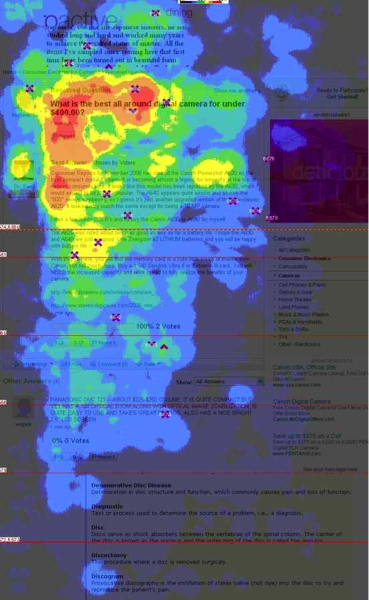
\includegraphics[width=0.75\textwidth]{images/heatmap}
\caption{Heatmap used to visualize where a users eyes spend their time}
\label{fig:heatmap}
\end{figure}

\paragraph{} In any evaluation, even if it’s for your coursework, look after your users:
\begin{itemize}
\item Follow any ethics guidelines eg don’t expose children to inappropriate material or excessive volume etc
\item Explain what you want and why
\item Treat them with respect – e.g. don’t roll your eyes if they get it all wrong
\item Let them withdraw if they have had enough
\item Reward them – be prepared to pay them – or if it’s a coursework reciprocate
\end{itemize}

\subsubsection{Interviews}

\paragraph{} Rather than just observing users - ask them what they think, why they approached tasks in the way they did etc. This can follow on from observation or, if you can’t observe for some reason, can be used as a substitute.

\subsubsection{Questionnaires}
\paragraph{} Everyone loves a good questionnaire. I know - you hate them - but for the developer they are easy and can reach a wide audience. The questionnaire returns can usually be analysed quantitatively (eg ``30\% got to the app icon first go'', ``18\% agreed that the text was easy to read''). Don’t just throw together some questions in five minutes - you only get one chance - study the theory of questionnaire design. It’s easy to make a mess of it and then you have lost your opportunity to gain valuable feedback.

\paragraph{} The following are some guidelines for good practice in questionnaire design:
\begin{itemize}
\item The complexity of your questionnaire and its language should take into account the age, education, competence, culture, and language abilities of respondents.
\item Consider using:
\item E-mail – fast, inexpensive, not anonymous.
\item Telephone – time consuming, not anonymous, may require skill, has to be short.
\item Face-to-face interview – slow, expensive, requires skill, best for small samples, qualitative studies.
\item Web-based – fast, inexpensive, can be anonymous, best for large surveys, for example use http://www.surveymonkey.com
\item Explain the purpose of the work – emphasise that it’s a worthwhile use of their time and they are contributing to something worthwhile and their feedback is important. Thank them too.
\item Keep it short and let them know how long it’ll take.
\item Use a good structure – group questions into sections. Let them skip or backtrack.
\item Keep response options simple, for example, use scales that provide useable granularity or consider a Lickert scale\footnote{\url{http://en.wikipedia.org/wiki/Likert_scale}}.
\item Be consistent don’t use a 5-point scale in one question and a 7-point in the next.
\item If you use a continuum scale with numbers for answer options, use a clear concept at the top and bottom of the scale (eg “on a scale of 1 to 5, how good is it? : where 1=very bad and 5=very good).
\item Use scales that are centred– don’t have one “bad” answer option and four shades of “good”.
\item Don’t force respondents into either/or answers if a neutral position is possible
\item ``Not applicable'' or ``don’t know'' responses should be available
\item Open responses are difficult for you to consolidate, so use them sparingly – but they can sometimes provide the best information, eg “what would you change?” but don’t force them to answer.
\end{itemize}

\subsubsection{Usability experts}
\paragraph{} Employ a trained usability expert and draw on their training and expertise. They would be considering the following heuristics (ie applying their experience gained/ knowledge to a problem) (Jones \& Marsden, 2006):

\begin{itemize}
\item Visibility of system status – does the user know where he is, what’s going on
\item Match between system and real-world – is the language right
\item User control and freedom – support undo/redo to help users who make mistakes
\item Consistency and standards – follow Android/ iPhone conventions
\item Error prevention – better to prevent than report errors eg restrict input
\item Flexibility and efficiency – responsiveness for users, let them tailor frequent actions
\item Aesthetic/ minimalist design – don’t overdo prompts etc
\item Recovery – help users recover if stuck or make a mistake
\item Help \& documentation – timely, appropriate help
\end{itemize}

\subsubsection{Experimental Evaluation}
\paragraph{} Here we try to evaluate our app with something similar. For example, compare Android  with iPhone. We pick one metric eg user errors and conduct a series of experiments such as asking the user to open a browser and find a site. You then use statistical analysis on recorded keypresses/ clicks to determine if the users were more likely to make an error using iPhone than Android then how long they took to overcome the error. 

\paragraph{} How do you know if the data is right about which would cause the fewest errors?  The skill is in the design of the experiment and the analysis tools used.

\subsection{Case Studies}
\subsubsection{Smart Diet}

\paragraph{} A group of researchers from Seoul, Korea developed a SmartDiet app then setup an experiment with 19 overweight people who used the app and a further 17 people who were asked to lose weight without the app\footnote{\url{http://jtt.rsmjournals.com/cgi/content/abstract/16/5/270}}. Overall, the researchers found that ``the SmartDiet mobile weight management application appears to contribute to weight loss in obese adults''.

\begin{figure}[H]
\centering
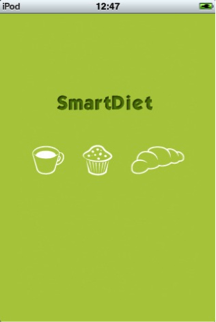
\includegraphics[width=0.5\textwidth]{images/smart-diet-1}
\caption{Smart Diet Launch Screen}
\label{fig:smart-diet-1}
\end{figure}

\begin{figure}[H]
\centering
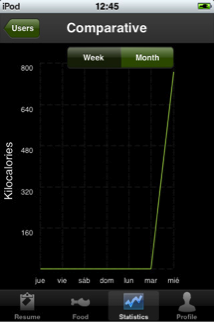
\includegraphics[width=0.5\textwidth]{images/smart-diet-2}
\caption{Smart Diet UI}
\label{fig:smart-diet-2}
\end{figure}

\subsubsection{M-AID}

\paragraph{} An app to support emergency medical treatment\footnote{\url{http://journals.lww.com/ejanaesthesiology/Fulltext/2007/06001/Evaluation_of_M_AID,_a_mobile_phone_first_aid.619.aspx}}

\paragraph{Background and Goal of Study} ``Cardiopulmonary resuscitation (CPR) by bystanders has been shown to reduce mortality due to sudden cardiac arrest when it is effectively performed.'' A mobile app detailing the steps for diagnosis and treatment was developed – called M-AID. The study wanted to see whether it was useful in an emergency situation.
Normally evaluation studies would need to compare against a control group. So if a new drug is developed they need one group to take the placebo to check whether the improvements are real or perceived.
Ethically, you can’t give 100 people the app and 100 people a dummy app and count the lives saved so they designed a scenario-based experiment – or simulated instances of cardiac arrest. The test group had the M-AID app and the control group didn’t have the app.

\paragraph{Materials and Methods} ``119 volunteers were randomly assigned either to the test or the control group. All participants had to manage the same emergency scenario - acute coronary syndrome leading to cardiac arrest. The participants were either equipped with a mobile phone running M-AID (test group) or had to handle the situation without any support (control group).''
The experiment was observed – with points allocated for each correct action taken. The scores were then compared. Some statistical levelling was introduced according to the participant’s medical training and experience. The participant’s mobile phone previous use and expertise was also recorded for the study. 
Results and Discussions: “The test group achieved a slightly higher average score that was not statistically significant (21.11 vs. 19.97; p = 0.302). In contrast, the performance of the individuals in the control group was significantly faster (2.41 min. vs. 4.24min; p < 0.001). Subgroup analysis showed that experienced mobile phone users performed significantly better than non experienced individuals, but not as good as participants with advanced first aid knowledge.”
\paragraph{Conclusions} ``Experience in the use of mobile phones is a precondition for the efficient use of the tested M-AID version. Furthermore, the software cannot replace skills acquisition by practical training. In a subgroup with experience in the handling of mobile phones and basic knowledge in CPR, the device improved performance of CPR.''

\begin{figure}[H]
\centering
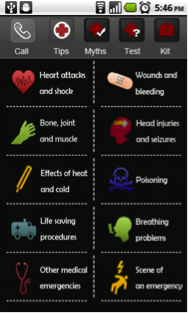
\includegraphics[width=0.5\textwidth]{images/m-aid-1}
\caption{M-AID main screen}
\label{fig:m-aid-1}
\end{figure}

\begin{figure}[H]
\centering
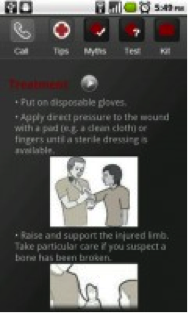
\includegraphics[width=0.5\textwidth]{images/m-aid-2}
\caption{Detail of the M-Aid advice}
\label{fig:m-aid-2}
\end{figure}

\section{Conclusions}
\paragraph{} Evaluation is largely the same as website/ desktop app evaluation but it has to include context. Don’t forget that the usability lab is less effective for mobile app evaluation than when you are evaluating a desktop app or a website. For mobile apps we have to move out to typical locations and situations: for example – inside, outside, in a crowd, in a park, on a bus. Think about both mobility and space. Engineer other interactions such as interruptions with phone and SMS events to see how your user can cope with your application while dealing with other typical events.

\paragraph{} Now your environment or context includes at night as well as during the day, at a rock concert, in a cathedral or in a supermarket. Never forget, however, that evaluation has to be proportionate. If you think you might sell 100 copies of your £0.79 app don’t go mad and pay users and psychologists to design a series of tests.



\section{Summary}
\paragraph{} We have looked at a range of topics related to the design and evaluation of mobile apps. You should now be able to:

\begin{itemize}
\item Use design patterns to communicate your designs
\item Use and understand platform guidelines
\item Evaluate your application
\end{itemize}

%\section{References \& Resources}


\chapter{Designing \& Engineering for Mobile}

\section{Aims}
\paragraph{} At the end of this topic you will be able to:

\begin{itemize}
\item Choose and follow a development methodology
\item Explain the mobile software development lifecycle
\item Perform Testing
\item Select the most appropriate development tools for your project
\end{itemize}


\paragraph{} We now focus on the practicalities of developing mobile apps in the wider context of software engineering and methodologies for creating effective and reliable software. Whilst in the last topic we considered the app in isolation with its own novel attributes in comparison to software on the server or desktop, instead, in this topic we consider how to engineer good apps and the methodologies we should follow if we are to build effective and reliable software. This is especially true if we consider thatin real-world development an app will rarely exist in isolation and will often be built by teams rather than individuals. An app will likely be part of a wider software system all of whose elements must work consistently together. Often an app will be developed which will work with data on the server, or services offered by 3rd parties, or will integrate closely with software on other platforms. Additionally, a team of developers working on a mobile app may have to work closely with developers building for other platforms or in different contexts. In order to make this process as smooth as possible, developers adopt software engineering methodologies and supporting tools to help them to work consistently and efficiently, to help them collaborate, and to ensure that their software artifacts are of high quality.

%SUPERHUB example.


\section{Methodologies}
\subsection{The Development Lifecycle}
\paragraph{} Developing mobile apps is simply software engineering in a specific application area. So what should our software engineering methods be?

\paragraph{} It is as if agile methods were made for mobile apps development. Short development cycles, building functionality and testing the app as you go along. The mantra is “test early, test often”. In agile, you can then stop when you have a product you can sell (or have run out of time and/ or money).

\paragraph{} Many software development projects start with a list of requirements generated from a customer/ client.  Often apps developers are drawing up their own requirements. Do a cost-benefit analysis on your project overall and of your requirements – prioritise them according to MOSCOW rules (those it must have, should have, could have and definitely won't have).

\begin{framed}
Planning to market your app? Don't forget any third-part requirements such as:
\begin{itemize}
\item Android License Agreement Requirements
\item Google Maps/ Third Party API Requirements
\item Android Market Requirements
\item Mobile Carrier/ Operator Requirements
\end{itemize}
\end{framed}

\paragraph{} A large, and underappreciated part of managing a software development project is managing risks. The biggest risk is your platform:
\begin{itemize}
\item handsets come and go at breakneck speed
\item handsets are customised for different markets \& regions
\item Android is at version 4.4 Kit-Kat– but for how long? each release is potentially significant to the success of your project
\item having access to the target handset – getting a pre-production handset might give you a competitive advantage
\end{itemize}

\paragraph{} Almost all of the most popular websites have migrated to phones – eg Facebook, BBC iPlayer – so simply expecting mobile users to browse to traditional websites is not seen as best practice for retaining your market share. Why's that?

\begin{itemize}
\item Small screen size – so need to customise
\item Limited/ uncomfortable data entry
\item Challenge of multitasking (eg Facebook is often running alongside MSN, YouTube on the desktop)
\item Representation of rich information (eg who's online, what's their strapline?)
\item Processor speed
\item Memory
\item Not always connected
\item Bandwidth
\item Expense of data roaming
\end{itemize}

\paragraph{} And from the users perspective?

\begin{itemize}
\item Interruptions likely – eg an SMS coming in
\item May be more public – more likely to be overlooked
\item May be more easily distracted
\item Need quick returns – some users download lots of apps but only use them infrequently
\end{itemize}

\subsubsection{Porting from a Desktop App} 
\paragraph{} 

\begin{itemize}
\item Avoid dialogs that pop up
\item Put interface elements under each other rather than side by side
\item To select a file – load them into a spinner
\item Test your app with one hand
\end{itemize}


\paragraph{} In summary, why are apps better than [web]sites for mobile? 
\begin{quote}
``Because the more impoverished the device, the more the design must be optimized for the platform's exact abilities, instead of bowing to a cross-platform common denominator.'' \footnote{\url{http://www.useit.com/alertbox/mobile-apps-initial-use.html}}
\end{quote}

\section{The Design Process}
\paragraph{} Jones \& Marsden (2006) define three activities involved in the design process:

\begin{itemize}
\item understanding users
\item developing prototype designs
\item evaluation – get feedback on your prototype and refine
\end{itemize}

\paragraph{} Overall, they state that interaction design should be “intensely participative and collaborative”. In most cases, to get the best results you can't go it alone – design reviews with peers and getting user feedback are useful in your app development.

\subsection{Understanding Users}
\paragraph{} To understand users you might want to conduct a field study. Ethnographers would study how people behave – taking into account collaboration, environment – observing how people behave in the situation in which the mobile app might be used. As an ethnographer you would be immersed in the environment and hopefully as invisible to the study group as possible.

\paragraph{} Do women and men behave differently? Course! Children and the elderly? The typical mobile user might not be an innovator and may not be a heavy desktop user. Your field study might observe different behaviours rather than making assumptions.

\paragraph{} Structured interviews/ direct questioning are more intrusive than ethnographic techniques, but are more direct and you can ask specific questions of your user group.

\paragraph{} How would these inform the design process? You could write up your observations \& interview results as scenarios (which are essentially use cases with more personality). This information would inform the prototyping stage as an indication of how the app could be used which in turn will inform the functionality required and the preferences in accessing/interacting with this functionality.

\subsection{Prototyping}

\paragraph{} The prototype is a basic working model of some part of an application which is either developed to get feedback into the requirements and/or design stage or which can be used as a step towards a final product. Developing a prototype is essential for mobile projects

\paragraph{} You can develop prototypes using mock up techniques (such mock-up.com, powerpoint templates, Visual Studio with Android plug-in, DroidDraw or Android App Inventor). 

\paragraph{} When developing your prototype, think about modelling the interaction with your final developed app. In particular (Jones \& Marsden,2006):
\begin{itemize}
\item direct manipulation – the iPod wheel is better than a scroll list
\item ecological use – would your context be useful eg location, other devices available to interact with eg over Bluetooth
\item design for maximum impact through minimum user effort
\item design for personalisation – people like to express their personality even though they are buying the same iPad as millions of others. Personalising makes them feel better towards their device/ app.
\item design for fun
\item design for one-handed use
\end{itemize}

\paragraph{} Add to that:

\begin{itemize}
\item design to be current OR functional (e.g. the Vuvuzela app for iPhone or the Bus Tracker – the former is use and throw away, the latter has currency through functionality)
\item use your mobile technology design guidelines\footnote{\url{http://developer.android.com/design/get-started/principles.html}} – e.g. Android offers a consistent framework for user interface components – well known ways of working with menus etc. Moving from one Android phone to another should be as easy as moving from one iPhone to another. There's no certification/ conformance rules yet but very strong guidelines on use of menus etc and icon style. They are protecting the brand.
\end{itemize}

\paragraph{} Guidelines are not just for display, guidelines are available for new gestures – the Android long press, iPhone’s pinch (now included in Android). Claiming to be intuitive, these new gestures are only intuitive if you first get shown them then all other devices use the same paradigm.
Some practical advice for apps developers:
\begin{itemize}
\item if possible, don't make users register first – hard lesson in ecommerce sites – let people put stuff in their basket before they fill out a form
\item try before you buy – or at least see before you buy
\item make it very simple – most app users are intermittent
\item include your icon design in this consideration – they might not use your app often – so make it easy for them to find when they do have the urge
\item design for performance – if you can get the work done by a server then farm it out, use efficient data structures, start fast, resume fast, use working progress tool
\item if possible, design for updates  - can extra features be plugged in without recompiling your app
\item design for interoperability  - can you work with other content providers
\item design in security – don't store or transmit non encrypted personal data
\item design for users on the go, being interrupted, having lots of apps
\end{itemize}

\subsection{Prototype Evaluation}
\paragraph{} Built your prototype? Now evaluate it – be ready to tear it up and start again – maybe you should let someone else evaluate? This is the hard bit – seeing your designs trashed. Develop a thick skin – and be a good listener. You don't always know best.

\paragraph{} Techniques include letting users loose on your prototype in a usability lab when they can be observed running through some sequence of operations. Then ask them to complete a questionnaire. You can also do some quantitative evaluation – how many keypresses are needed to run through the sequence, how long did it take etc

\paragraph{} You need enough functionality to make this prototype evaluation meaningful, however you don't want to complete your application only to find it's frustrating to use and won't sell.

\section{Development \& Testing}

\subsection{Development}
\paragraph{} Once you have established that your design is good – start developing. There’s nothing much that is particularly unique to Android app development:

\begin{itemize}
\item Pick the best IDE, i.e. Android Studio
\item Work long hours (but not silly hours)
\item FAQs and forums – if you haven’t got a google account, get one
\item Use code reviews to share good practice
\end{itemize}

\subsection{The Philosophy}

\paragraph{} The Android development philosophy includes insisting that you should keep resources external to your code where possible. Resources include strings and images. You can then look after them independently of your code. It also means that when a new device comes along with a screen shape you hadn’t anticipated you can make changes easily. Essentially: store everything in your resource directory (/res in Android Studio).


\begin{figure}[H]%[htb]
\centering
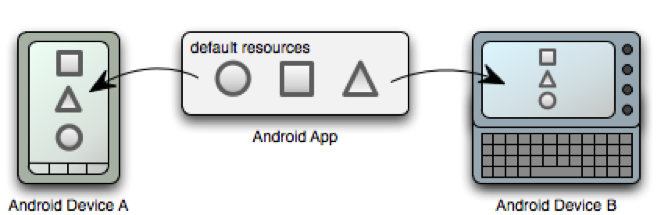
\includegraphics[width=\textwidth]{images/res_sharing}
\caption{Sharing Resources between devices}
\label{fig:res_sharing}
\end{figure}

\begin{figure}[H]%[htb]
\centering
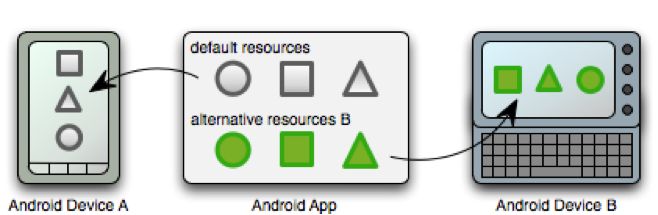
\includegraphics[width=\textwidth]{images/res_separate}
\caption{Using alternative resources for different devices}
\label{fig:res_separate}
\end{figure}


\begin{figure}[H]%[htb]
\centering
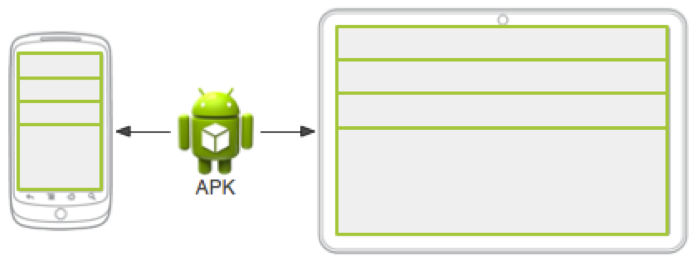
\includegraphics[width=\textwidth]{images/res-layout-default}
\caption{Resources resized - each using the default layout}
\label{fig:res-layout-defaultt}
\end{figure}

\begin{figure}[H]%[htb]
\centering
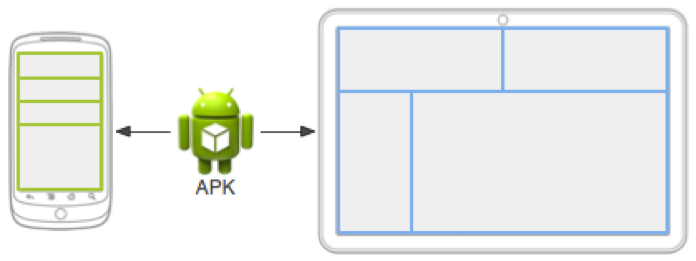
\includegraphics[width=\textwidth]{images/res-layout-alt}
\caption{Alternative layouts for tablets}
\label{fig:res-layout-alt}
\end{figure}

\subsection{Testing}
\paragraph{} As with agile methods, test early and often. To that we can add, for mobile apps, - try to test on your target kit as early as possible. Use a range of tools – such as JUnit and Android’s Monkey Exerciser. Monkey\footnote{\url{http://developer.android.com/guide/developing/tools/monkey.html}} is a command line tool which sends a random stream of events to your application to see how it deals with them. It can be used to stress test and can run on an emulator or a device. You can configure it to set up the number of events that should be created, to identify the packages you want to test, to establish event types and their frequencies and how it should react to an error. 

\begin{framed}
Why ``monkey''? From the infinite monkey theorem – if you have enough monkeys, at enough typewriters, eventually one of them will type the complete works of Shakespeare.
\end{framed}



\section{Tooling}
\paragraph{} There are many tools that can support you in creating robust and maintainable mobile apps. If we take Android as our example, there are the pre-requisites, basically Java and the Android SDK. You can develop for Android entirely at the command-line but there are also Integrated Development Environments (IDEs) which can help you. The two main IDEs are the Android SDK based on Eclipse which was historically been the default IDE for Android development and Android Studio which because the default IDE, according to the Android project, in December 2014. It is recommended that developers new to Android should work with Android Studio unless they are already higly experienced with Eclipse. Even then, it is difficult to say for how long the Eclipse Android plugins will continue to be supported.

However, you should always be aware that whilst these tools can help and support you, they are not a substitute for knowing the platform and the problem you are trying to solve, as well as possible. One advantage that IDEs to offer however is a way to explore the Android system by exploiting the visual editor, for drawing and prototyping layouts and exploring the view options without having to remember the XML that defines each option, and by exploiting the auto-complete feature which will suggest potential methods and objects from the Android libraries and your current project.

%\subsection{Integrated Development Environments}
%\subsubsection{Android Studio}
%\paragraph{} 

%\subsubsection{Eclipse with AndroidSDK plugin}
%\paragraph{}

\subsubsection{Build Control: Gradle \& Maven}
\paragraph{} Behind the more superficial UI differences between Studio and Eclipse, are some more substantial differences. One of the most important is the build system. Studio uses Gradle whereas Eclipse uses maven. An advantage of the new approach using Gradle is that various project parameters can be set in the Gradle build file which can then be used to complete your Android Manifest. This essentially means that you can have multiple Android apps built from the same codebase and build system, each targetting different API levels or working differently according to their target platform. This increases the flexibility of what was already a flexible system for developing apps to run across a wide range of platforms. Given that Android Studio uses Gradle, and Android Studio is the `tier one' development platform for Android, we should really get to grips with Gradle.

\subsection{Version Control}
\paragraph{} Version control is fundamental whether you are working individually or as part of a team. A good version control system, such as Git, will manage all of your resources and source code, enabling you to track changes between them, to track the history of each, and to maintain multiple versions of your app. Distributed version control, with sufficient tools for reconciling different and divergent versions, is essential when working with a team of developers, enabling each to work on their own part of the codebase and providing support to reconcile any `incompatible' difference between the versions. By incompatible versions we mean where developers have made alterations to the same piece of code and a decision has to be made about which to choose over the other, or whether refactoring to include both alterations is required. 

\subsubsection{Git}
\paragraph{} Unless you are already experienced with an alternative version control system, it is recommended that you use Git. There is a very good chance that during your career you will work in a software development team that uses this tool. Whilst Android Studio supports a range of version control tools, look under the ``VCS'' menu and you will see support for CVS, Subversion, Mercurial, and Git, Studio also supports GitHub which makes it straightforward to share your code, as open source for example, but also to create an offsite backup of your project.

\subsection{Best Practises}
\paragraph{} Due to the complicated Android hardware landscape there are many potential issues and pitfalls associated with developing app, particularly if you wish to reliable target a wide range of devices. The Android documentation provides a number of best practises\footnote{\url{https://developer.android.com/guide/practices/compatibility.html}} which it is worth becoming familiar with.

\paragraph{} For example,

\begin{itemize}
\item Use density-independent measurements in your layouts, so your specifications will scale along with the screen.
\item When putting together layouts, use relative widths and heights instead of absolute values.
\item Putting in several versions of the same image file, tailored to different screen densities, can also be a good idea.
\end{itemize}

\paragraph{} Because the Android eco-system is developing so rapidly it is worth trying to stay on top of the agreed best-practises and the differences between new versions of the platform. Whilst the platform APIs are quite rigid, to all intents and practises, if a feature is not supported by a particular API level then it is not available for that target, best practises are more malleable. It is always worth retaining a critical approach with respect to best practises and asking yourself, `does this still apply?', there may be a better way but it might be that nobody has realised it yet. Therefore best-practises can evolve and improve over time as the platform develops. This can be annoying, but means that the platform is still trying to innovate and be the best that it can be, even if sometime this means there must be major changes.

\section{Summary}
\paragraph{}

\paragraph{} In this topic we covered: 
\begin{itemize}
\item Designing your apps
\item Developing and testing your apps
\end{itemize}

\section{Directed Study}
\begin{itemize}
\item Read Chapters 4-6  of Mobile Interaction Design: Matt Jones \& Gary Marsden, Wiley, 2006
\item Read Chapters 18-19 of Android Wireless Application Development: Shane Condor \& Lauren Darcey, Addison-Wesley, 2010
\item Have a look at Microsoft’s guidelines  for their “metro style\footnote{\url{http://msdn.microsoft.com/library/windowsphone/develop/fa00461b-abe1-41d1-be87-0b0fe3d3389d(v=vs.105).aspx}}” for mobile apps and highlight any that wouldn’t be applicable to Android apps and visit the developers website http://developer.android.com for tips.
\item Check your understanding of the topic by answering the following:
\begin{enumerate}
\item Have you used design guidelines before (for example, in designing a website)? Can those be applied here?
\item What do interaction designers mean by “ethnography”?
\item If you are designing an app for older people, how would you contact a user group?
\item Why do you think SMS worked – beyond anyone's expectations?
\item Name 5 design rules built in to Android. Start by reading the Android design guidelines\footnote{\url{http://developer.android.com/guide/practices/ui_guidelines/index.html}}
\end{enumerate}
\item If you have time, build up an archive of your design ideas and inspiration from elsewhere – screen shots of killer apps, colour palettes, screen shots of your own work – critique your collection.
\end{itemize}


%\section{References \& Resources}

\chapter{Persisting Your Data in a Mobile World}

\section{Aims}
\paragraph{} At the end of this topic you will be able to:

\begin{itemize}
\item 
\end{itemize}

\paragraph{} Once you have come up with a great app idea there are various processes that you start to work through. The design process, and the methodology that supports it, are two important processes. One of the outcomes that stem from these early processes is an awareness of the data that your app will use. In this respect app development is {\emph{just}} like any other software development project. You have to determine what data is important to your app, how it is structured, and how it will be stored.

\paragraph{} As with nearly every other topic in this area, app devlopment doesn't simplify the process of designing and producing software but piles on special cases. Data storage is no exception. Whilst developing for the desktop or server generally assumes hard-drive technology, at least for the moment, there are relatively few choices to be made about data storage; essentially will my data be stored in files on disk or in a database. Mobile devices offer various types of storage and your app may well end up storing and using data from a variety of locations. These options include:

\begin{itemize}
\item Shared Preferences - Private key-value storage of primitive data types (such as int, double, float, string, etc)
\item Internal Storage - Private ``documents'' directory for file storage which can only be accessed by your application
\item External Storage - Public file storage, usually on an expandable storage device such as an SD card
\item Database - Private data storage in a database on the device
\item Network - Storage of data on remote servers, either through a custom built API or using a data storage service. ({\emph{NB. We include this point merely for completeness. We will look at remote storage as a part of the connectivity topic because it is intimately connected with the skills required to transmit data to and remote Application Programming Interfaces (APIs) and use networking.}})
\end{itemize}

\paragraph{} In addition to the above mentioned data storage options, additional apps can be installed locally to provide hybrid data storage functionality. For example, installation of a stand-alone DB, for example a NoSQL DB, to provide DB services different to the built in DB (e.g. SQLite) and which is accessed as another app or service running locally. NB. This kind of approach can complicate deployment of your app, as it will now require the presence of an additional, non-standard, service running on your target device, but also potentially offers functionality that you might not otherwise be able to easily achieve otherwise.


\section{Preferences}
\paragraph{}

\subsection{Saving Files}
\paragraph{} Most mobile platforms, with the notable exception of Apple's iOS, offerinternal and external storage for user data. Usually this means that the internal storage is built into the device and the external storage is some kind of expandable external hardware such as SD-cards. Android devices, for example, offer both internal and external storage and there are some small differences between the two which developers should be aware of, these are summarised as follows:

\begin{description}
\item[Internal]
    \begin{itemize}
    \item Always accessible
    \item Accessible only by the `owning' app, i.e. your apps files are only available to your app (by default - this behaviour can be overridden)
    \item System automatically removes all of an app's files when the app is uninstalled
    \end{itemize}
\item[External] 
    \begin{itemize}
    \item Not necessarily accessible. Might be on a removeable medium and therefore might not currently be attached
    \item World readable so you can't guarantee, be default, that other apps might not read your app's files
    \item Files are not necessarily removed on uninstallation. You have to take measures to ensure that your apps files are removed from this storage on uninstallation
    \end{itemize}
\end{description}

\subsection{Internal/Onboard}
\paragraph{} Internal storage usually refers to the built-in storage offered by your device. This is in contrast to the expandable storage offered by technologies like SD-cards, compact flash, USB, etc. 

\subsection{External/SD-Card}
\paragraph{} In this topic we will concentrate on the SD-card as an external and expandable data storage medium. The distinction between internal and external storage, at least on Android is a holdover from the early days of the platform when a device would include a small amount of internal storage plus external expandable storage. Modern devices now commonly incorporate sufficient internal memory that expandable storage is not as critically important as it used to be. Despite this, even if an Android device does not have expandable storage then it will likely have the internal storage devided, or partitioned, into two parts, ``internal'' and ``external''.

\paragraph{} It should be noted however that Apple does not offer expandable storage on any of their iOS devices.


\section{Databases}
\paragraph{}

\section{Summary}
\paragraph{}

\section{References \& Resources}
\paragraph{}




\begin{comment}
\part{Case Studies}
\chapter{Daybook}
\label{daybook}
\paragraph{}
\end{comment}

\begin{comment}
\appendix
\chapter{}
\label{}
\paragraph{} 
\end{comment}

\backmatter

\bibliographystyle{plain}

\bibliography{bib/mobile-apps}

\end{document}

